\documentclass[11pt,a4paper,dvipsnames]{article}
\usepackage[margin=2.5cm]{geometry}
\usepackage{iohk}
\usepackage{microtype}
\usepackage{mathpazo} % nice fonts
\usepackage{amsmath}
\usepackage{amssymb}
\usepackage{amsthm}
\usepackage{latexsym}
\usepackage{mathtools}
\usepackage{stmaryrd}
\usepackage{extarrows}
\usepackage{slashed}
\usepackage[colon]{natbib}
\usepackage[unicode=true,pdftex,pdfa,colorlinks=true]{hyperref}
\usepackage{xcolor}
\usepackage[capitalise,noabbrev,nameinlink]{cleveref}
\usepackage{float}
\floatstyle{boxed}
\restylefloat{figure}
\usepackage{tikz}
\usepackage{booktabs}
\usepackage{enumerate}


%%
%% Package `semantic` can be used for writing inference rules.
%%
\usepackage{semantic}
%% Setup for the semantic package
\setpremisesspace{20pt}

%%
%% Types
%%
\newcommand{\Nothing}{\ensuremath{\Diamond}}
\newcommand{\N}{\ensuremath{\mathbb{N}}}
\newcommand{\Npos}{\ensuremath{\mathbb{N}^{+}}}
\newcommand{\Z}{\ensuremath{\mathbb{Z}}}
\newcommand{\R}{\ensuremath{\mathbb{R}}}
\newcommand{\Rnn}{\ensuremath{\mathbb{R}^{\geq 0}}}
\newcommand{\Tx}{\type{Tx}}
\newcommand{\TxBody}{\type{TxBody}}
\newcommand{\Ix}{\type{Ix}}
\newcommand{\TxId}{\type{TxId}}
\newcommand{\Addr}{\type{Addr}}
\newcommand{\UTxO}{\type{UTxO}}
\newcommand{\Wdrl}{\type{Wdrl}}
\newcommand{\Value}{\type{Value}}
\newcommand{\Coin}{\type{Coin}}
\newcommand{\PParams}{\type{PParams}}
\newcommand{\Slot}{\type{Slot}}
\newcommand{\SlotsPerEpoch}{\mathsf{SlotsPerEpoch}}
\newcommand{\SlotsPerKESPeriod}{\mathsf{SlotsPerKESPeriod}}
\newcommand{\Duration}{\type{Duration}}
\newcommand{\StakePools}{\type{StakePools}}
\newcommand{\StakeKeys}{\type{StakeKeys}}
\newcommand{\Seed}{\type{Seed}}
\newcommand{\seedOp}{\star}
\newcommand{\EEnt}{\type{EEnt}}

\newcommand{\DCert}{\type{DCert}}
\newcommand{\DCertRegKey}{\type{DCert_{regkey}}}
\newcommand{\DCertDeRegKey}{\type{DCert_{deregkey}}}
\newcommand{\DCertDeleg}{\type{DCert_{delegate}}}
\newcommand{\DCertRegPool}{\type{DCert_{regpool}}}
\newcommand{\DCertRetirePool}{\type{DCert_{retirepool}}}
\newcommand{\PoolParam}{\type{PoolParam}}
\newcommand{\UTxOState}{\ensuremath{\type{UTxOState}}}
\newcommand{\ledgerState}{\ensuremath{\type{ledgerState}}}

\newcommand{\AddrRWD}{\type{Addr_{rwd}}}
\newcommand{\AddrB}{\type{Addr_{base}}}
\newcommand{\AddrP}{\type{Addr_{ptr}}}
\newcommand{\AddrE}{\type{Addr_{enterprise}}}
\newcommand{\AddrBS}{\type{Addr_{bootstrap}}}
\newcommand{\Ptr}{\type{Ptr}}
\newcommand{\DState}{\type{DState}}
\newcommand{\DWEnv}{\type{DWEnv}}
\newcommand{\DPSEnv}{\type{DPSEnv}}
\newcommand{\DPEnv}{\type{DPEnv}}
\newcommand{\DEnv}{\type{DEnv}}
\newcommand{\PEnv}{\type{PEnv}}
\newcommand{\DPState}{\type{DPState}}
\newcommand{\PState}{\type{PState}}
\newcommand{\DCertBody}{\type{DCertBody}}
\newcommand{\TData}{\type{TData}}
\newcommand{\DPoolReap}{\ensuremath{\type{poolreap}}}
\newcommand{\UPIState}{\type{UPIState}}
\newcommand{\UpdatePayload}{\type{UpdatePayload}}

%% Adding witnesses
\newcommand{\TxIn}{\type{TxIn}}
\newcommand{\TxOut}{\type{TxOut}}
\newcommand{\VKey}{\type{VKey}}
\newcommand{\VKeyEv}{\type{VKey_{ev}}}
\newcommand{\VKeyGen}{\type{VKey_G}}
\newcommand{\SKey}{\type{SKey}}
\newcommand{\SKeyEv}{\type{SKey_{ev}}}
\newcommand{\HashKey}{\type{HashKey}}
\newcommand{\KeyPair}{\type{KeyPair}}
\newcommand{\KeyPairEv}{\type{KeyPair_{ev}}}
\newcommand{\Sig}{\type{Sig}}
\newcommand{\Data}{\type{Data}}
%% Adding delegation
\newcommand{\Epoch}{\type{Epoch}}
\newcommand{\KESPeriod}{\type{KESPeriod}}
%% Blockchain
\newcommand{\Gkeys}{\var{G_{keys}}}
\newcommand{\Block}{\type{Block}}
\newcommand{\SlotId}{\type{SlotId}}
\newcommand{\UTxOEnv}{\type{UTxOEnv}}
\newcommand{\CEEnv}{\type{CEEnv}}
\newcommand{\CEState}{\type{CEState}}
\newcommand{\BDEnv}{\type{BDEnv}}
\newcommand{\BDState}{\type{BDState}}
\newcommand{\LEnv}{\type{LEnv}}
\newcommand{\LState}{\type{LState}}

%%
%% Functions
%%
\newcommand{\txins}[1]{\fun{txins}~ \var{#1}}
\newcommand{\txouts}[1]{\fun{txouts}~ \var{#1}}
\newcommand{\txcerts}[1]{\fun{txcerts}~ \var{#1}}
\newcommand{\txid}[1]{\fun{txid}~ \var{#1}}
\newcommand{\outs}[1]{\fun{outs}~ \var{#1}}
\newcommand{\values}[1]{\fun{values}~ #1}
\newcommand{\ubalance}[1]{\fun{ubalance}~ \var{#1}}
\newcommand{\txttl}[1]{\fun{txttl}~ \var{#1}}
\newcommand{\firstSlot}[1]{\fun{firstSlot}~ \var{#1}}
\newcommand{\deposits}[2]{\fun{deposits}~ \var{#1} ~ \var{#2}}
\newcommand{\decayedKey}[4]{\fun{decayedKey}~ \var{#1}~ \var{#2}~ \var{#3}~ \var{#4}}
\newcommand{\decayedTx}[3]{\fun{decayedTx}~ \var{#1}~ \var{#2}~ \var{#3}}
\newcommand{\keyRefund}[6]{\fun{keyRefund}~ {#1}~{#2}~{#3}~\var{#4}~\var{#5}~\var{#6}}
\newcommand{\refund}[4]{\fun{refund}~ \var{#1}~ \var{#2}~ {#3}~ {#4}}
\newcommand{\keyRefunds}[3]{\fun{keyRefunds}~ \var{#1}~ \var{#2}~ \var{#3}}
\newcommand{\consumed}[4]{\fun{consumed}~ \var{#1}~ \var{#2}~ \var{#3}~ \var{#4}}
\newcommand{\produced}[2]{\fun{produced}~ \var{#1}~ \var{#2}}
\newcommand{\applyFun}[2]{\fun{#1}~\var{#2}}

\newcommand{\RegKey}[1]{\textsc{RegKey}(#1)}
\newcommand{\DeregKey}[1]{\textsc{DeregKey}(#1)}
\newcommand{\Delegate}[1]{\textsc{Delegate}(#1)}
\newcommand{\RegPool}[1]{\textsc{RegPool}(#1)}
\newcommand{\RetirePool}[1]{\textsc{RetirePool}(#1)}
\newcommand{\cwitness}[1]{\fun{cwitness}~ \var{#1}}
\newcommand{\dpool}[1]{\fun{dpool}~ \var{#1}}
\newcommand{\poolParam}[1]{\fun{poolParam}~ \var{#1}}
\newcommand{\retire}[1]{\fun{retire}~ \var{#1}}
\newcommand{\addrRw}[1]{\fun{addr_{rwd}}~ \var{#1}}
\newcommand{\epoch}[1]{\fun{epoch}~\var{#1}}
\newcommand{\kesPeriod}[1]{\fun{kesPeriod}~\var{#1}}
\newcommand{\dcerts}[1]{\fun{dcerts}~ \var{#1}}
\newcommand{\pps}[1]{\fun{pps}~ \var{#1}}

%% UTxO witnesses
\newcommand{\inputs}[1]{\fun{inputs}~ \var{#1}}
\newcommand{\txwits}[1]{\fun{txwits}~ \var{#1}}
\newcommand{\verify}[3]{\fun{verify} ~ #1 ~ #2 ~ #3}
\newcommand{\sign}[2]{\fun{sign} ~ #1 ~ #2}
\newcommand{\verifyEv}[4]{\fun{verify_{ev}} ~ #1 ~ #2 ~ #3 ~ #4}
\newcommand{\signEv}[3]{\fun{sign_{ev}} ~ #1 ~ #2 ~ #3}
\newcommand{\serialised}[1]{\llbracket \var{#1} \rrbracket}
\newcommand{\hashKey}[1]{\fun{hashKey}~ \var{#1}}
\newcommand{\txbody}[1]{\fun{txbody}~ \var{#1}}
\newcommand{\txfee}[1]{\fun{txfee}~ \var{#1}}
\newcommand{\txwdrls}[1]{\fun{txwdrls}~ \var{#1}}
\newcommand{\minfee}[2]{\fun{minfee}~ \var{#1}~ \var{#2}}
\newcommand{\slotminus}[2]{\var{#1}~-_{s}~\var{#2}}
\DeclarePairedDelimiter\floor{\lfloor}{\rfloor}
% wildcard parameter
\newcommand{\wcard}[0]{\underline{\phantom{a}}}
%% Adding ledgers...
\newcommand{\utxo}[1]{\fun{utxo}~ #1}
%% Delegation
\newcommand{\delegatesName}{\fun{delegates}}
\newcommand{\delegates}[3]{\delegatesName~#1~#2~#3}
\newcommand{\dwho}[1]{\fun{dwho}~\var{#1}}
\newcommand{\depoch}[1]{\fun{depoch}~\var{#1}}
\newcommand{\dval}{\ensuremath{d_{\mathsf{val}}}}
%% Delegation witnesses
\newcommand{\dbody}[1]{\fun{dbody}~\var{#1}}
\newcommand{\dwit}[1]{\fun{dwit}~\var{#1}}
%% Blockchain
\newcommand{\bwit}[1]{\fun{bwit}~\var{#1}}
\newcommand{\bslot}[1]{\fun{bslot}~\var{#1}}
\newcommand{\bbody}[1]{\fun{bbody}~\var{#1}}
\newcommand{\bhbody}[1]{\fun{bhbody}~\var{#1}}
\newcommand{\bdlgs}[1]{\fun{bdlgs}~\var{#1}}
%% ledgerstate constants
\newcommand{\genesisId}{\ensuremath{Genesis_{Id}}}
\newcommand{\genesisTxOut}{\ensuremath{Genesis_{Out}}}
\newcommand{\genesisUTxO}{\ensuremath{Genesis_{UTxO}}}
\newcommand{\emax}{\ensuremath{\mathsf{E_{max}}}}

\newcommand{\unitInterval}{\ensuremath{[0,~1]}}
\newcommand{\unitIntervalNonNull}{\ensuremath{(0,~1]}}
\newcommand{\nonnegReals}{\ensuremath{[0,~\infty)}}
\newcommand{\posReals}{\ensuremath{(0,~\infty)}}

\theoremstyle{definition}
\newtheorem{definition}{Definition}[section]
\newtheorem{property}{Property}[section]

\newcommand{\leteq}{\ensuremath{\mathrel{\mathop:}=}}

\begin{document}

\hypersetup{
  pdftitle={A Formal Specification of the Cardano Ledger},
  breaklinks=true,
  bookmarks=true,
  colorlinks=false,
  linkcolor={blue},
  citecolor={blue},
  urlcolor={blue},
  linkbordercolor={white},
  citebordercolor={white},
  urlbordercolor={white}
}


  \cleardoublepage%
  \tableofcontents%
  \listoffigures%
  \clearpage%

  \begin{changelog}
        \change{2019/10/08}{Jared Corduan, Polina Vinogradova and Matthias G\"udemann}{FM (IOHK)}{Initial version (0.1).}
        \change{2019/10/08}{Kevin Hammond}{FM (IOHK)}{Added cover page.}
      \end{changelog}
      \clearpage%
\begin{landscape}
\floatstyle{plain}
\restylefloat{figure}
\begin{figure*}
\includegraphics[scale=0.65]{d8-depends.pdf}
\caption{Positioning of this Deliverable.}
\end{figure*}
\end{landscape}
\floatstyle{boxed}
\restylefloat{figure}
\cleardoublepage
% \begin{center}
%   \large{Executive Summary}
% \end{center}

% \noindent
% This document provides a formal specification of the Cardano ledger for use in the Shelley implementation.
% It is intended to form the basis for an executable specification that will be the basis of the initial
% release.
% \cleardoublepage
\renewcommand{\thepage}{\arabic{page}}
\setcounter{page}{1}

\title{A Formal Specification of the Cardano Ledger}

\author{Jared Corduan  \\ {\small \texttt{jared.corduan@iohk.io}} \\
   \and Polina Vinogradova \\ {\small \texttt{polina.vinogradova@iohk.io}} \\
   \and Matthias G\"udemann  \\ {\small \texttt{matthias.gudemann@iohk.io}}}

%\date{}

\maketitle

\begin{abstract}
This document provides a formal specification of the Cardano ledger for use in the upcoming Shelley implementation.
It is intended to underpin a Haskell executable specification that will be the basis of the initial
Shelley release, and represents a core design and quality assurance document.
It will be used to define properties and tests, and to provide the basis for strong formal assurance
using mathematical proof techniques.
The document defines the rules for extending the ledger with transactions
that will affect both UTxO and stake delegation.
Key properties that have been identified include ...
% This will serve as the specification for random generators of transactions
% which adhere to the rules presented here, and that will.
\end{abstract}

\section*{List of Contributors}
\label{acknowledgements}

Nicol\'as Arqueros,
Nicholas Clarke,
Duncan Coutts,
Ruslan Dudin,
Sebastien Guillemot,
Vincent Hanquez,
Ru Horlick,
Michael Hueschen,
Yun Lu,
Philipp Kant,
Jean-Christophe Mincke,
Damian Nadales,
Nicolas Di Prima.


\tableofcontents
\listoffigures

\section{Introduction}
\label{sec:introduction-shelley}

This document is a formal specification of the functionality of the ledger
on the blockchain. The blockchain layer of the
protocol and the interaction between the ledger and the blockchain
layer is presented in a separate document, see~\cite{shelley_consensus}. The details of the
background and the larger context
for the design decisions formalized in this document are presented
in~\cite{delegation_design}

In this work,
we present important properties any implementation of the ledger must have.
Specifically, we model the following aspects
of the functionality of the ledger on the blockchain:

\begin{description}
\item[Preservation of value] Every coin in the system is accounted for,
  and the total amount is unchanged by every transaction and epoch change.
  In particular, every coin is accounted for by one of the following categories:
  \begin{itemize}
    \item Circulation (UTxO)
    \item Deposit pot
    \item Fee pot
    \item Reserves (monetary expansion)
    \item Rewards (account addresses)
    \item Reward pot (undistributed)
    \item Treasury
  \end{itemize}
\item[Witnesses] Authentication of parts of the transaction data by means of
  cryptographic entities (such as signatures and private keys) contained in
  these transactions.
\item[Delegation] Validity of delegation certificates, which delegate
  block-signing rights.
\item[Stake] Staking rights associated to an address.
\end{description}

While the blockchain protocol is a reactive system driven by the arrival
of blocks causing updates to the ledger, the formal description is a collection
of rules which is a
static description of what a \textit{valid ledger} is. The specifics of the
semantics we use to define and apply
the rules we present in this document are explained in detail in
\cite{small_step_semantics}. A valid ledger state can only
reached by applying a sequence of inference rules, and any valid ledger state
is reachable by applying some sequence of these rules.

The structure of the rules we give here is such that their application is
deterministic. That is, given a specific initial state and relevant environmental
constants, there is no ambiguity
about which rule should be applied at any given time (i.e.~which state
transition is allowed take place). This is an important property which reflects
the reality of the implementation --- the blockchain evolves in a particular way
given some user activity and the passage of time, and its behaviour is
never unexpected.

\section{Notation}
\label{sec:notation-shelley}

The transition system is explained in \cite{small_step_semantics}.

\begin{description}
  \item[Powerset] Given a set $\type{X}$, $\powerset{\type{X}}$ is the set of all
    the subsets of $X$.
  \item[Sequences] Given a set $\type{X}$, $\seqof{\type{X}}$ is the set of
    sequences having elements taken from $\type{X}$. The empty sequence is
    denoted by $\epsilon$, and given a sequence $\Lambda$, $\Lambda; \type{x}$ is
    the sequence that results from appending $\type{x} \in \type{X}$ to
    $\Lambda$.
  \item[Functions] $A \to B$ denotes a \textbf{total function} from $A$ to $B$.
    Given a function $f$ we write $f~a$ for the application of $f$ to argument
    $a$.
  \item[Inverse Image] Given a function $f: A \to B$ and $b\in B$, we write
    $f^{-1}~b$ for the \textbf{inverse image} of $f$ at $b$, which is defined by
    $\{a \mid\ f a =  b\}$.
  \item[Maps and partial functions] $A \mapsto B$ denotes a \textbf{partial
    function} from $A$ to $B$, which can be seen as a map (dictionary) with
    keys in $A$ and values in $B$. Given a map $m \in A \mapsto B$, notation
    $a \mapsto b \in m$ is equivalent to $m~ a = b$.
  \item[Map Operations] Figure~\ref{fig:notation:nonstandard}
    describes some non-standard map operations.
  \item[Relations] A relation on $A\times B$ is a subset of $A\times B$.
    Both maps and functions can be thought of as relations.
    A function $f:A\to B$ is a relation consisting of pairs $(a, f(a))$ such that $a\in A$.
    A map $m: A\mapsto B$ is a relation consisting of pairs $(a, b)$ such that
    $a\mapsto b \in m$.
    Given a relation $R$ on $A\times B$, we define the inverse relation $R^{-1}$ to be
    all pairs $(b, a)$ such that $(a, b)\in R$. Similarly, given a function $f:A\to B$ we
    define inverse relation $f^{-1}$ to consist of all pairs $(f(a), a)$.
    Finally, given two relations $R\subseteq A\times B$ and $S\subseteq B\times C$,
    we define the compostion $R\circ S$ to be all pairs $(a, c)$ such that
    $(a, b)\in R$ and $(b, c)\in S$ for some $b\in B$.
  \item[Option type] An option type in type $A$ is denoted as $A^? = A + \Nothing$. The
    $A$ case corresponds to a case when there is a value of type $A$ and the $1$
    case corresponds to a case when there is no value.

\end{description}

In Figure~\ref{fig:notation:nonstandard}, we specify the notation we use in
the rest of the document.

\begin{figure}[htb]
  \begin{align*}
    \var{set} \restrictdom \var{map}
    & = \{ k \mapsto v \mid k \mapsto v \in \var{map}, ~ k \in \var{set} \}
    & \text{domain restriction}
    \\
    \var{set} \subtractdom \var{map}
    & = \{ k \mapsto v \mid k \mapsto v \in \var{map}, ~ k \notin \var{set} \}
    & \text{domain exclusion}
    \\
    \var{map} \restrictrange \var{set}
    & = \{ k \mapsto v \mid k \mapsto v \in \var{map}, ~ v \in \var{set} \}
    & \text{range restriction}
    \\
    \var{map} \subtractrange \var{set}
    & = \{ k \mapsto v \mid k \mapsto v \in \var{map}, ~ v \notin \var{set} \}
    & \text{range exclusion}
    \\
    A \triangle B
    & = (A \setminus B) \cup (B \setminus A)
    & \text{symmetric difference}
    \\
    M \unionoverrideRight N
    & = (\dom N \subtractdom M)\cup N
    & \text{union override right}
    \\
    M \unionoverrideLeft N
    & = M \cup (\dom M \subtractdom N)
    & \text{union override left}
    \\
    M \unionoverridePlus N
    & = (M \triangle N)
    \cup \{k\mapsto v_1+v_2\mid {k\mapsto v_1}\in M \land {k\mapsto v_2}\in N \}
    & \text{union override plus} \\
    & & \text{(for monoidal values)}\\
  \end{align*}
  \caption{Non-standard map operators}
  \label{fig:notation:nonstandard}
\end{figure}

\clearpage

\section{Cryptographic primitives}
\label{sec:crypto-primitives-shelley}

Figure~\ref{fig:crypto-defs-shelley} introduces the cryptographic abstractions used in
this document. we begin by listing the abstract types, which are meant to
represent the corresponding concepts in cryptography. Only the functionality
explicitly stated in the figures below is assumed to be within the scope of this paper.
That is, their exact
implementation remains open to interpretation and we do not rely on
any additional properties derived from the study or implementation of public key
cryptography outside this work. The types and rules we give here are needed in
order to guarantee certain security properties of the delegation process, which
we discuss later.

The cryptographic concepts required for the formal definition of witnessing
include public-private key pairs, one-way functions, signatures and
multi-signature scripts. The constraint we introduce states that a signature of
some data signed with a (private) key is only correct whenever we can verify it
using the corresponding public key.

Besides basic cryptographic abstractions, we also make use of some abstract
data storage properties in this document in order to build necessary definitions
and make judgement calls about them.

Abstract data types in this paper are essentially placeholders with names
indicating the data types they are meant to represent in an implementation.
Derived types are made up of data structures (i.e.~products, lists, finite
maps, etc.) built from abstract types. The underlying structure of a data type
is implementation-dependent and furthermore, the way the data is stored on
physical storage can vary as well.

Serialization is a physical manifestation of data on a given storage device.
In this document, the properties and rules we state involving serialization are
assumed to hold true independently of the storage medium and style of data
organization chosen for an implementation.

\begin{figure}[htb]
  \emph{Abstract types}
  %
  \begin{equation*}
    \begin{array}{r@{~\in~}lr}
      \var{sk} & \SKey & \text{private signing key}\\
      \var{vk} & \VKey & \text{public verifying key}\\
      \var{hk} & \KeyHash & \text{hash of a key}\\
      \sigma & \Sig  & \text{signature}\\
      \var{d} & \Data  & \text{data}\\
      \var{script} & \Script & \text{multi-signature script} \\
      \var{hs} & \HashScr & \text{hash of a script}
    \end{array}
  \end{equation*}
  \emph{Derived types}
  \begin{equation*}
    \begin{array}{r@{~\in~}lr}
      (sk, vk) & \KeyPair & \text{signing-verifying key pairs}
    \end{array}
  \end{equation*}
  \emph{Abstract functions}
  %
  \begin{equation*}
    \begin{array}{r@{~\in~}lr}
      \hashKey{} & \VKey \to \KeyHash
                 & \text{hashKey function} \\
                 %
      \fun{verify} & \powerset{\left(\VKey \times \Data \times \Sig\right)}
                   & \text{verification relation}\\
                   %
      \fun{sign} & \SKey \to \Data \to \Sig
                 & \text{signing function}\\
      \fun{hashScript} & \Script \to \HashScr & \text{hash a serialized script}
    \end{array}
  \end{equation*}
  \emph{Constraints}
  \begin{align*}
    & \forall (sk, vk) \in \KeyPair,~ d \in \Data,~ \sigma \in \Sig \cdot
    \sign{sk}{d} = \sigma \implies \verify{vk}{d}{\sigma}
  \end{align*}
  \emph{Notation for serialized and verified data}
  \begin{align*}
    & \serialised{x} & \text{serialised representation of } x\\
    & \mathcal{V}_{\var{vk}}{\serialised{d}}_{\sigma} = \verify{vk}{d}{\sigma}
    & \text{shorthand notation for } \fun{verify}
  \end{align*}
  \caption{Cryptographic definitions}
  \label{fig:crypto-defs-shelley}
\end{figure}

When we get to the blockchain layer validation, we will use
key evolving signatures according to the MMM scheme \citep{cryptoeprint:2001:034}.
Figure~\ref{fig:kes-defs-shelley} introduces the additional cryptographic abstractions
needed for KES.


\begin{figure}[htb]
  \emph{Abstract types}
  %
  \begin{equation*}
    \begin{array}{r@{~\in~}lr}
      \var{sk} & \N \to \SKeyEv & \text{private signing keys}\\
      \var{vk} & \VKeyEv & \text{public verifying key}\\
    \end{array}
  \end{equation*}
  \emph{Notation for evolved signing key}
  \begin{align*}
    & \var{sk_n} = \var{sk}~n & n\text{-th evolution of }sk
  \end{align*}
  \emph{Derived types}
  \begin{equation*}
    \begin{array}{r@{~\in~}lr}
      (sk_n, vk) & \KeyPairEv & \text{signing-verifying key pairs}
    \end{array}
  \end{equation*}
  \emph{Abstract functions}
  %
  \begin{equation*}
    \begin{array}{r@{~\in~}lr}
      \fun{verify_{ev}} & \powerset{\left(\VKey \times \N \times \Data \times \Sig\right)}
                        & \text{verification relation}\\
                        %
      \fun{sign_{ev}} & \SKey \to \N \to \Data \to \Sig
                      & \text{signing function}\\
    \end{array}
  \end{equation*}
  \emph{Constraints}
  \begin{align*}
    & \forall n\in\N, (sk_n, vk) \in \KeyPairEv, ~ d \in \Data,~ \sigma \in \Sig \cdot \\
    & ~~~~~~~~\signEv{sk}{n}{d} = \sigma \implies \verifyEv{vk}{n}{d}{\sigma}
  \end{align*}
  \emph{Notation for verified KES data}
  \begin{align*}
    & \mathcal{V}^{\mathsf{KES}}_{\var{vk}}{\serialised{d}}_{\sigma}^n
        = \verifyEv{vk}{n}{d}{\sigma}
    & \text{shorthand notation for } \fun{verify_{ev}}
  \end{align*}
  \caption{KES Cryptographic definitions}
  \label{fig:kes-defs-shelley}
\end{figure}
\clearpage

\section{Addresses}
\label{sec:addresses}

Addresses are described in section 4.2 of the delegation design document \cite{delegation_design}.
The types needed for the addresses are defined in Figure~\ref{fig:defs:addresses}.
There are three types of UTxO addresses:
\begin{itemize}
  \item Base addresses, $\AddrB$,
        containing the hash of a payment key and the hash of a staking key,
  \item Pointer addresses, $\AddrP$,
        containing the hash of a payment key and a pointer to a stake key registration certificate,
  \item Enterprise addresses, $\AddrE$,
        containing only the hash of a payment key (and which have no staking rights).
\end{itemize}
Together, these three address types make up the $\Addr$ type, which will be used
in transaction outputs in Section~\ref{sec:utxo}.

Note that for security, privacy and usability reasons, the staking (delegating)
key pair associated with an address should be different from its payment key pair.
Before the stake key is registered and delegated to an existing stake pool,
the payment key can be used for transactions, though it will not receive rewards from staking.
Once a stake key is registered, the shorter pointer addresses can generated.

Finally, there is an account style address $\AddrRWD$ which contains the hash of a staking key.
These account addresses will only be used for receiving rewards from the proof of
stake leader election.  Apendix A of \cite{delegation_design} explains this design choice.
The mechanism for transferring rewards from these accounts will be explained in
Section~\ref{sec:utxo} and follows \cite{chimeric}.

\begin{figure*}[hbt]
  \emph{Abstract types}
  %
  \begin{equation*}
    \begin{array}{r@{~\in~}lr}
      slot & \Slot & \text{absolute slot}\\
      ix & \Ix & \text{index}\\
    \end{array}
  \end{equation*}
  %
  \emph{Derived types}
  %
  \begin{equation*}
    \begin{array}{r@{~\in~}l@{\qquad=\qquad}lr}
      \var{(s,t,c)}
      & \Ptr
      & \Slot\times\Ix\times\Ix
      & \text{certificate pointer}
      \\
      \var{addr}
      & \AddrB
      & \HashKey_{pay}\times\HashKey_{stake}
      & \text{base address}
      \\
      \var{addr}
      & \AddrP
      & \HashKey_{pay}\times\Ptr
      & \text{pointer address}
      \\
      \var{addr}
      & \AddrE
      & \HashKey_{pay}
      & \text{enterprise address}
      \\
      \var{addr}
      & \Addr
      & \AddrB \uniondistinct \AddrP \uniondistinct \AddrE
      & \text{output address}
      \\
      \var{acct}
      & \AddrRWD
      & \HashKey_{stake}
      & \text{reward account}
      \\
    \end{array}
  \end{equation*}
  %
  \emph{Accessor Functions}
  %
  \begin{equation*}
    \begin{array}{r@{~\in~}lr}
      \fun{paymentHK} & \Addr \to \HashKey_{pay}
                      & \text{hash of payment key from addr}\\
      \fun{stakeHK_b} & \AddrB \to \HashKey_{stake}
                      & \text{hash of stake key from base addr}\\
      \fun{stakeHK_r} & \AddrRWD \to \HashKey_{stake}
                      & \text{hash of stake key from reward account}\\
      \fun{addrPtr} & \AddrP \to \Ptr
                    & \text{pointer from pointer addr}\\
    \end{array}
  \end{equation*}
  %
  \emph{Constructor Functions}
  %
  \begin{equation*}
    \begin{array}{r@{~\in~}lr}
      \fun{addr_{rwd}}
        & \HashKey_{stake} \to \AddrRWD
        & \text{construct a reward account}
    \end{array}
  \end{equation*}
  %
  \emph{Constraints}
  %
  \begin{equation*}
    \var{hk_1} = \var{hk_2} \iff \fun{addr_{rwd}}~\var{hk_2} = \fun{addr_{rwd}}~\var{hk_2}
    ~~~ \left( \fun{addr_{rwd}} \text{ is injective} \right)
  \end{equation*}
  \caption{Definitions used in Addresses}
  \label{fig:defs:addresses}
\end{figure*}

\clearpage

\section{Protocol Parameters}
\label{sec:protocol-parameters}

The rules for the ledger depend on several parameters and are contained in the $\PParams$ type
defined in Figure~\ref{fig:defs:protocol-parameters}.

The type $\Coin$ is defined as an alias for the integers.
Negative values will not be allowed in UTxO outputs or reward accounts,
and $\Z$ is only chosen over $\N$ for its additive inverses.

The $\fun{minfee}$ function calculates the minimum fee that must be paid by a transaction.
This value depends on the protocol parameters and the size of the transaction.

Two time related types are introduced, $\Epoch$ and $\type{Duration}$.
A $\type{Duration}$ is the difference between two slots, as given by $\slotminus{}{}$.

Two global constants are defined, $\SlotsPerEpoch$ and $\SlotsPerKESPeriod$,
representing the number of slots in an epoch/KES period.  Cycles will be used in
the key evolving signatures.  As global constants, these values can only be
changed by updating the software.

Lastly, there are two functions, $\fun{epoch}$ and $\fun{firstSlot}$ for converting
between epochs and slots and one function $\fun{kesPeriod}$ for getting the cycle of a slot.

\begin{figure*}[htb]
  \emph{Abstract types}
  %
  \begin{equation*}
    \begin{array}{r@{~\in~}lr}
      \var{fparams} & \type{FeeParams} & \text{min fee parameters}\\
      \var{dur} & \Duration & \text{difference between slots}\\
      \var{epoch} & \Epoch & \text{epoch} \\
      \var{kesPeriod} & \KESPeriod & \text{KES period} \\
    \end{array}
  \end{equation*}
  %
  \emph{Derived types}
  %
  \begin{equation*}
    \begin{array}{r@{~\in~}l@{\qquad=\qquad}lr}
      \var{coin}
      & \Coin
      & \Z
      & \text{unit of value}
      \\
    \end{array}
  \end{equation*}
  %
  \emph{Protocol Parameters}
  %
  \begin{equation*}
    \PParams =
    \left(
      \begin{array}{r@{~\in~}lr}
        \var{fparams} & \type{FeeParams} & \text{min fee parameters}\\
        \var{keyDeposit} & \Coin & \text{stake key deposit}\\
        \var{keyMinRefund} & \unitInterval & \text{stake key min refund}\\
        \var{keyDecayRate} & \nonnegReals & \text{stake key decay rate}\\
        \var{poolDeposit} & \Coin & \text{stake pool deposit}\\
        \var{poolMinRefund} & \unitInterval & \text{stake pool min refund}\\
        \var{poolDecayRate} & \nonnegReals & \text{stake pool decay rate}\\
        \var{E_{max}} & \Epoch & \text{epoch bound on pool retirement}\\
        \var{n_{opt}} & \Npos & \text{desired number of pools}\\
        \var{a_0} & \posReals & \text{pool influence}\\
        \tau & \unitInterval & \text{treasury expansion}\\
        \rho & \unitInterval & \text{monetary expansion}\\
        \var{maxBHSize} & \N & \text{max block header size}\\
        \var{maxBBSize} & \N & \text{max block body size}\\
        \var{activeSlotCoeff} & \unitInterval & f\text{ in \cite{ouroboros_praos}}\\
      \end{array}
    \right)
  \end{equation*}
  %
  \emph{Accessor Functions}
  %
  \begin{center}
    \fun{fparams},
    \fun{keyDeposit},
    \fun{keyMinRefund},
    \fun{keyDecayRate},
    \fun{poolDeposit},
    \fun{poolMinRefund},
    \fun{poolDecayRate},
    \fun{emax},
    \fun{nopt},
    \fun{influence},
    \fun{tau},
    \fun{rho},
    \fun{maxBHSize},
    \fun{maxBBSize},
    \fun{activeSlotCoeff},
  \end{center}
  %
  \emph{Abstract Functions}
  %
  \begin{equation*}
    \begin{array}{r@{~\in~}lr}
      \fun{minfee} & \PParams \to \Tx \to \Coin
                   & \text{minimum fee calculation}
      \\
      (\slotminus{}{}) & \Slot \to \Slot \to \Duration
                       & \text{duration between slots}
    \end{array}
  \end{equation*}
  %
  \emph{Global Constants}
  %
  \begin{equation*}
    \begin{array}{r@{~\in~}lr}
      \SlotsPerEpoch & \N & \text{slots per epoch} \\
      \SlotsPerKESPeriod & \N & \text{slots per KES period} \\
    \end{array}
  \end{equation*}
  %
  \emph{Derived Functions}
  %
  \begin{align*}
    \fun{epoch} & \in ~ \Slot \to \Epoch & \text{epoch of a slot}
    \\
    \fun{epoch} & ~\var{slot} = \var{slot}~\mathsf{div}~\SlotsPerEpoch
    \\
    \\
    \fun{firstSlot} & \in ~ \Epoch \to \Slot
               & \text{first slot of an epoch}
    \\
    \fun{firstSlot} & ~\var{e} = \var{e}~\cdot~\SlotsPerEpoch
    \\
    \\
    \fun{kesPeriod} & \in ~ \Slot \to \KESPeriod & \text{KES period of a slot}
    \\
    \fun{kesPeriod} & ~\var{slot} = \var{slot}~\mathsf{div}~\SlotsPerKESPeriod
  \end{align*}
  %
  \caption{Definitions used in Protocol Parameters}
  \label{fig:defs:protocol-parameters}
\end{figure*}

\clearpage

\section{Transactions}
\label{sec:transactions}

Transactions are defined in Figure~\ref{fig:defs:utxo-shelley}.
A transaction body, $\TxBody$, is made up of six pieces:

\begin{itemize}
  \item A set of transaction inputs.
    The $\TxIn$ derived type identifies an output from a previous transaction.
    It consists of a transaction id and an index to uniquely identify the output.
  \item An indexed collection of transaction outputs.
    The $\TxOut$ type is an address paired with a coin value.
  \item A list of certificates, which will be explained in detail in
    Section~\ref{sec:delegation-shelley}.
  \item A transaction fee. This value will be added to the fee pot and eventually handed out
    as stake rewards.
  \item A time to live. A transaction will be deemed invalid if processed after this slot.
  \item A mapping of reward account withdrawals.  The type $\Wdrl$ is a finite map that maps
    a reward address to the coin value to be withdrawn. The coin value must be equal
    to the full value contained in the account. Explicitly stating these values ensures
    that error messages can be precise about why a transaction is invalid.
\end{itemize}
A transaction, $\Tx$, is a transaction body together with:

\begin{itemize}
  \item A collection of witnesses, represented as a finite map from payment verification keys
    to signatures.
\end{itemize}

Additionally, the $\UTxO$ type will be used by the ledger state to store all the
unspent transaction outputs. It is a finite map from transaction inputs
to transaction outputs that are available to be spent.

Finally, $\fun{txid}$ computes the transaction id of a given transaction.
This function must produce a unique id for each unique transaction.

\begin{figure*}[htb]
  \emph{Abstract types}
  %
  \begin{equation*}
    \begin{array}{r@{~\in~}lr}
      \var{txid} & \TxId & \text{transaction id}\\
    \end{array}
  \end{equation*}
  \emph{Derived types}
  %
  \begin{equation*}
    \begin{array}{r@{~\in~}l@{\qquad=\qquad}lr}
      (\var{txid}, \var{ix})
      & \TxIn
      & \TxId \times \Ix
      & \text{transaction input}
      \\
      (\var{addr}, c)
      & \type{TxOut}
      & \Addr \times \Coin
      & \text{transaction output}
      \\
      \var{utxo}
      & \UTxO
      & \TxIn \mapsto \TxOut
      & \text{unspent tx outputs}
      \\
      \var{wdrl}
      & \Wdrl
      & \AddrRWD \mapsto \Coin
      & \text{reward withdrawal}
    \end{array}
  \end{equation*}
  %
  \emph{Transaction Types}
  %
  \begin{equation*}
    \begin{array}{r@{~\in~}l@{\qquad=\qquad}l}
      \var{txbody}
      & \TxBody
      & \powerset{\TxIn} \times (\Ix \mapsto \TxOut) \times \seqof{\DCert}
        \times \Coin \times \Slot \times \Wdrl
      \\
      \var{tx}
      & \Tx
      & \TxBody \times (\VKey \mapsto \Sig)
      \\
    \end{array}
  \end{equation*}
  %
  \emph{Accessor Functions}
  \begin{equation*}
    \begin{array}{r@{~\in~}lr}
      \fun{txins} & \Tx \to \powerset{\TxIn} & \text{transaction inputs} \\
      \fun{txouts} & \Tx \to (\Ix \mapsto \TxOut) & \text{transaction outputs} \\
      \fun{txcerts} & \Tx \to \seqof{\DCert} & \text{delegation certificates} \\
      \fun{txfee} & \Tx \to \Coin & \text{transaction fee} \\
      \fun{txttl} & \Tx \to \Slot & \text{time to live} \\
      \fun{txwdrls} & \Tx \to \Wdrl & \text{withdrawals} \\
      \fun{txbody} & \Tx \to \TxBody & \text{transaction body}\\
      \fun{txwits} & \Tx \to (\VKey \mapsto \Sig) & \text{witnesses} \\
    \end{array}
  \end{equation*}
  %
  \emph{Abstract Functions}
  \begin{equation*}
    \begin{array}{r@{~\in~}lr}
      \txid{} & \Tx \to \TxId & \text{compute transaction id}\\
    \end{array}
  \end{equation*}
  \caption{Definitions used in the UTxO transition system}
  \label{fig:defs:utxo-shelley}
\end{figure*}

\clearpage

\section{UTxO}
\label{sec:utxo}

Some of the functions related to scripts, datums and collateral need
to be adjusted for the new features. Most of these adjustments are
self-explanatory. Note that the new $\fun{collOuts}$ function
generates a single output with an index $| \txouts{txb} |$. This is to
avoid potential confusion for transactions spending that output. Note
that $\TxId$ can only hold integers up to $2^{16} - 1$. In case of an
overflow, we let this number be $2^{16} - 1$.

\begin{figure*}[htb]
  \emph{Functions}
  %
  \begin{align*}
    & \fun{isTwoPhaseScriptAddress} : \Tx \to \hldiff{\UTxO} \to \Addr \to \Bool \\
    & \fun{isTwoPhaseScriptAddress}~tx~\hldiff{utxo}~a = \\
    &\quad\begin{cases}
        \True  & a \in \AddrScr \land \fun{validatorHash}~a \mapsto s \in \fun{txscripts}~tx~\hldiff{utxo} \land s \in \ScriptPhTwo \\
        \False & \text{otherwise}
      \end{cases}
    \nextdef
    & \fun{collOuts} : \TxBody \to \UTxO \\
    & \fun{collOuts}~txb =
      \begin{cases}
        \emptyset                                                      & \fun{collRet}~txb = \Nothing \\
        \{ (\txid{txb}, | \txouts{txb} |) \mapsto \fun{collRet}~txb \} & \text{otherwise}
      \end{cases}
    \nextdef
    & \fun{collBalance} : \TxBody \to \UTxO \to \Value \\
    & \fun{collBalance}~txb~utxo = \fun{ubalance}~(\var{utxo}|_{\fun{collInputs}~{txb}}) - \fun{ubalance}~(\fun{collOuts}~txb)
    \nextdef
    & \fun{feesOK} : \PParams \to \Tx \to \UTxO \to \Bool  \\
    & \fun{feesOK}~\var{pp}~tx~utxo = \\
    &~~      \minfee{pp}{tx} \leq \txfee{tx} \wedge (\fun{txrdmrs}~tx \neq \Nothing \Rightarrow \\
    &~~~~~~~~~~\forall (a, \wcard, \wcard) \in \fun{range}~(\fun{collInputs}~tx \restrictdom \var{utxo}), a \in \AddrVKey \\
    &~~~~~~\wedge \fun{adaOnly}~\var{balance} \\
    &~~~~~~\wedge \var{balance} \geq \hldiff{\lceil \txfee{txb} * \fun{collateralPercent}~pp / 100 \rceil} \\
    &~~~~~~\wedge \hldiff{(\fun{txcoll}~tx \neq \Nothing) \Rightarrow \var{balance} = \fun{txcoll}~tx} \\
    &~~~~~~\wedge \fun{collInputs}~{tx} \neq \emptyset) \\
    &~~      \where \\
    & ~~~~~~~ \var{balance}=\hldiff{\fun{collBalance}~tx~utxo}
  \end{align*}
  \caption{Functions related to fees and collateral}
  \label{fig:functions:utxo}
\end{figure*}

\begin{figure*}
  \begin{align*}
    & \fun{getDatum} : \Tx \to \UTxO \to \ScriptPurpose \to \seqof{\Datum} \\
    & \fun{getDatum}~{tx}~{utxo}~{sp} =
      \begin{cases}
        [\var{d}] & \var{sp} \in \TxIn, (\_, \_, h, \_) \in \var{utxo}~\var{sp},~ \var{d}\in\fun{txdats}~(\fun{txwits}~tx)~\var{h} \\
        [\var{d}] & \hldiff{\var{sp} \in \TxIn, (\_, \_, d, \_) \in \var{utxo}~\var{sp},~ \var{d} \in \Datum} \\
        \epsilon  & \text{otherwise}
      \end{cases}
    \nextdef
    & \fun{refScripts} : \Tx \to \hldiff{\UTxO} \to \ScriptHash \pto \Script \\
    & \fun{refScripts}~tx~utxo = \{ \fun{hash}~s \mapsto s \mid (\_, \_, \_, s) \in \var{utxo}~(\fun{spendInputs}~tx \cup \fun{refInputs}~tx)\}
    \nextdef
    & \fun{txscripts} : \Tx \to \hldiff{\UTxO} \to \ScriptHash \pto \Script \\
    & \fun{txscripts}~tx~utxo = \fun{txwitscripts}~tx \cup \hldiff{\fun{refScripts}~tx~utxo}
    \nextdef
    & \fun{allOuts} : \Tx \to \powerset{\TxOut} \\
    & \fun{allOuts}~tx = \range \txouts{tx} \cup \fun{collRet}~tx
    \nextdef
    & \fun{languages} : \Tx \to \UTxO \to \powerset{\Language} \\
    & \fun{languages}~tx~utxo =
      \{\fun{language}~s \mid s \in \range (\fun{txscripts}~tx~\hldiff{utxo}) \cap \ScriptPhTwo\}
    \nextdef
    & \fun{allowedLanguages} : \Tx \to \UTxO \to \powerset{\Language} \\
    & \fun{allowedLanguages}~tx~utxo = \\
    & \begin{cases}
        \emptyset                   & \text{if}~\exists (a, \_, \_, \_) \in os, a \in \AddrBS \\
        \{ \PlutusVII \}            & \text{if}~\exists (\_, \_, d, s) \in os, d \in \Datum \lor s \neq \Nothing \lor \fun{refInputs}~tx \neq \emptyset \\
        \{ \PlutusVI, \PlutusVII \} & \text{otherwise}
      \end{cases} \\
    & \where \var{os} = \range \txouts{tx} \cup \var{utxo}~(\fun{spendInputs}~tx \cup \fun{refInputs}~tx)
  \end{align*}
  \caption{Functions related to scripts}
  \label{fig:functions:data}
\end{figure*}

\begin{figure}[htb]
  \begin{equation}
    \inference[Scripts-Yes]
    {
    \var{txb}\leteq\txbody{tx} &
    \var{sLst} := \fun{collectTwoPhaseScriptInputs}~\var{pp}~\var{tx}~\var{utxo}
    \\~\\
    {
      \begin{array}{r}
        \var{slot} \\
        \var{pp} \\
        \var{genDelegs} \\
      \end{array}
    }
    \vdash \var{pup} \trans{\hyperref[fig:rules:update]{ppup}}{\fun{txup}~\var{tx}} \var{pup'}
    \\~\\
    \var{refunded} \leteq \keyRefunds{pp}{txb}
    \\
    \var{depositChange} \leteq
      \fun{totalDeposits}~{pp}~\var{poolParams}~(\txcerts{txb})~-~\var{refunded}
    \\~\\
    \fun{isValid}~\var{tx} = \fun{evalScripts}~\var{tx}~\var{sLst} = \True
    }
    {
    \begin{array}{l}
      \var{slot}\\
      \var{pp}\\
      \var{poolParams}\\
      \var{genDelegs}\\
    \end{array}
      \vdash
      \left(
      \begin{array}{r}
        \var{utxo} \\
        \var{deposits} \\
        \var{fees} \\
        \var{pup} \\
      \end{array}
      \right)
      \trans{utxos}{tx}
      \left(
      \begin{array}{r}
        \varUpdate{\var{(\fun{spendInputs}~txb \subtractdom \var{utxo}) \cup \outs{txb}}}  \\
        \varUpdate{\var{deposits} + \var{depositChange}} \\
        \varUpdate{\var{fees} + \txfee{txb}} \\
        \varUpdate{\var{pup'}} \\
      \end{array}
      \right) \\
    }
  \end{equation}
  \begin{equation}
    \inference[Scripts-No]
    {
    \var{txb}\leteq\txbody{tx} &
    \var{sLst} := \fun{collectTwoPhaseScriptInputs}~\var{pp}~\var{tx}~\var{utxo} \\
    \hldiff{\var{collateralFees} := \fun{valueToCoin}~(\fun{collBalance}~txb~utxo)}
    \\
    ~
    \\
    \fun{isValid}~\var{tx} = \fun{evalScripts}~\var{tx}~\var{sLst} = \False
    }
    {
    \begin{array}{l}
      \var{slot}\\
      \var{pp}\\
      \var{poolParams}\\
      \var{genDelegs}\\
    \end{array}
      \vdash
      \left(
      \begin{array}{r}
        \var{utxo} \\
        \var{deposits} \\
        \var{fees} \\
        \var{pup} \\
      \end{array}
      \right)
      \trans{utxos}{tx}
      \left(
      \begin{array}{r}
        \varUpdate{\var{(\fun{collInputs}~{txb} \subtractdom \var{utxo})} \cup \hldiff{\fun{collOuts}~txb}}  \\
        \var{deposits} \\
        \varUpdate{\var{fees} + \hldiff{\var{collateralFees}}} \\
        \var{pup} \\
      \end{array}
      \right)
    }
  \end{equation}
  \caption{State update rules}
  \label{fig:rules:utxo-state-upd}
\end{figure}

In the UTXO rule, we switch from a manual estimation of the size consumed by $\UTxO$ entries to an estimation using the serialization. However, since the $\TxIn$ used as a key in the $\UTxO$ map is not part of the serialization, we need to account for it manually. By itself it is $40$ bytes, but we add another $120$ bytes of overhead for the in-memory representation of Haskell data.

\begin{figure}[htb]
  \begin{equation}
    \inference[UTxO-inductive]
    {
      \var{txb}\leteq\txbody{tx} &
      \fun{ininterval}~\var{slot}~(\fun{txvldt}~{txb}) &
      \var{(\wcard, i_f)}\leteq\fun{txvldt}~{tx} \\~\\
      \Nothing \notin \{\fun{txrdmrs}~\var{tx}, i_f\} \Rightarrow \fun{epochInfoSlotToUTCTime}~\mathsf{EI}~\mathsf{SysSt}~i_f \neq \Nothing \\
      \fun{spendInputs}~txb \neq \emptyset
      & \fun{feesOK}~pp~tx~utxo
      \\
      \fun{spendInputs}~txb \cup \fun{collInputs}~txb \cup \hldiff{\fun{refInputs}~{tx}} \subseteq \dom \var{utxo} \\
      \consumed{pp}{utxo}{txb} = \produced{pp}{poolParams}~{txb}
      \\~\\
      \mathsf{adaID}\notin \supp {\fun{mint}~tx} \\~\\
      \forall txout \in \hldiff{\fun{allOuts}~txb}, \\
      \fun{getValue}~txout \geq \fun{inject}~(\hldiff{(\fun{serSize}~txout + 160) * \fun{coinsPerUTxOByte}~pp}) \\~
      \\
      \forall txout \in \hldiff{\fun{allOuts}~txb},\\
      \fun{serSize}~(\fun{getValue}~txout) \leq \fun{maxValSize}~pp \\~
      \\
      \forall (\wcard\mapsto (a,~\wcard)) \in \hldiff{\fun{allOuts}~txb}, a \in \AddrBS \Rightarrow \fun{bootstrapAttrsSize}~a \leq 64 \\
      \forall (\wcard\mapsto (a,~\wcard)) \in \hldiff{\fun{allOuts}~txb}, \fun{netId}~a = \NetworkId
      \\
      \forall (a\mapsto\wcard) \in \txwdrls{txb}, \fun{netId}~a = \NetworkId \\
      (\fun{txnetworkid}~\var{txb} = \NetworkId) \vee (\fun{txnetworkid}~\var{txb} = \Nothing)
      \\~\\
      \fun{txsize}~{tx}\leq\fun{maxTxSize}~\var{pp} \\~\\
      \fun{totExunits}~{tx} \leq \fun{maxTxExUnits}~{pp} &  \| \fun{collInputs}~{tx} \| \leq \fun{maxCollateralInputs}~{pp}
      \\
      ~
      \\
      {
        \begin{array}{c}
          \var{slot}\\
          \var{pp}\\
          \var{poolParams}\\
          \var{genDelegs}\\
        \end{array}
      }
      \vdash
      {
        \left(
          \begin{array}{r}
            \var{utxo} \\
            \var{deposits} \\
            \var{fees} \\
            \var{pup}\\
          \end{array}
        \right)
      }
      \trans{utxos}{\var{tx}}
      {
        \left(
          \begin{array}{r}
            \var{utxo'} \\
            \var{deposits'} \\
            \var{fees'} \\
            \var{pup'}\\
          \end{array}
        \right)
      }
    }
    {
      \begin{array}{l}
        \var{slot}\\
        \var{pp}\\
        \var{poolParams}\\
        \var{genDelegs}\\
      \end{array}
      \vdash
      \left(
      \begin{array}{r}
        \var{utxo} \\
        \var{deposits} \\
        \var{fees} \\
        \var{pup}\\
      \end{array}
      \right)
      \trans{utxo}{tx}
      \left(
      \begin{array}{r}
        \varUpdate{\var{utxo'}}  \\
        \varUpdate{\var{deposits'}} \\
        \varUpdate{\var{fees'}} \\
        \varUpdate{\var{pup'}}\\
      \end{array}
      \right)
    }
  \end{equation}
  \caption{UTxO inference rules}
  \label{fig:rules:utxo-babbage}
\end{figure}

To the UTXOW rule, in addition to the changes required by the new
features, we add a check that all scripts and datums involved in the
transaction are well-formed. We forbid transactions that try to
execute $\PlutusVI$ scripts and use the new features which can't be
translated to $\PlutusVI$'s $\TxInfo$ (reference inputs, inline datums
and reference scripts). We also forbid transactions that involve Byron 
addresses.

\begin{figure}
  \begin{equation}
    \label{eq:utxo-witness-inductive-babbage}
    \inference[UTxO-witG]
    {
      \var{txb}\leteq\txbody{tx} &
      \var{txw}\leteq\fun{txwits}~{tx} \\
      (utxo, \wcard, \wcard, \wcard) \leteq \var{utxoSt} \\
      \var{witsKeyHashes} \leteq \{\fun{hashKey}~\var{vk} \vert \var{vk} \in
      \dom (\txwitsVKey{txw}) \}\\
      \var{inputHashes}\leteq \left\{ h \,\middle|
        {
          \begin{array}{l}
            (a, \_, h) \in \range(\var{utxo}|_{\fun{spendInputs}~tx}) \\
            \fun{isTwoPhaseScriptAddress}~tx~\hldiff{utxo}~a \\
          \end{array}
        }
      \right\} - \hldiff{\Datum} \\~\\
      \var{neededHashes}\leteq \{ h \mid (\_, h) \in \fun{scriptsNeeded}~\var{utxo}~txb\} \\
      \forall \var{s} \in (\fun{txscripts}~txw~\hldiff{utxo~\var{neededHashes}}) \cap \ScriptPhOne,
      \fun{validateScript}~\var{s}~\var{tx}\\~\\
      \var{neededHashes} - \hldiff{\dom (\fun{refScripts}~tx~utxo)} = \dom (\fun{txwitscripts}~txw) \\~\\
      \var{inputHashes} \subseteq_{\{h \mid (\wcard, \wcard, h)\in\fun{allOuts}~tx \cup \hldiff{\var{utxo}~(\fun{refInputs}~{tx})}\}} \dom (\fun{txdats}~{txw})  \\~\\
      \\~\\
      \dom (\fun{txrdmrs}~tx) = \left\{ \fun{rdptr}~txb~sp \,\middle|
        {
          \begin{array}{l}
            (sp,h) \in \fun{scriptsNeeded}~\var{utxo}~txb \\
            \fun{txscripts}~{txw}~\hldiff{utxo}~h \in \ScriptPhTwo
          \end{array}
        } \right\}
      \\~\\
      \var{txbodyHash}\leteq\fun{hash}~(\txbody{tx}) \\
      \forall \var{vk} \mapsto \sigma \in \txwitsVKey{tx},
      \mathcal{V}_{\var{vk}}{\serialised{txbodyHash}}_{\sigma} \\
      \fun{witsVKeyNeeded}~{utxo}~{tx}~{genDelegs} \subseteq witsKeyHashes
      \\~\\
      genSig \leteq
      \left\{
        \fun{hashKey}~gkey \vert gkey \in\dom{genDelegs}
      \right\}
      \cap
      \var{witsKeyHashes}
      \\
      \left\{
        c\in\txcerts{txb}~\cap\DCertMir
      \right\} \neq\emptyset \implies \vert genSig\vert \geq \Quorum
      \\~\\
      \var{adh}\leteq\fun{txADhash}~\var{txb}
      &
      \var{ad}\leteq\fun{auxiliaryData}~\var{tx}
      \\
      (\var{adh}=\Nothing \land \var{ad}=\Nothing)
      \lor
      (\var{adh}=\fun{hashAD}~\var{ad})
      \\~\\
      \hldiff{\forall x \in \range (\fun{txdats}~txw) \cup \range (\fun{txwitscripts}~txw)} \\
      \hldiff{\cup \bigcup_{(\_, \_, d, s) \in \hldiff{\fun{allOuts}~txb}} \{s, d\} \cup \fun{scripts}~(\fun{auxiliaryData}~tx),} \\
      \hldiff{x \in \Script \cup \Datum \Rightarrow \fun{isWellFormed}~x}
      \\~\\
      \fun{languages}~tx~\hldiff{utxo} \subseteq \dom(\fun{costmdls}~pp) \cap \fun{allowedLanguages}~tx~utxo \\
      \fun{scriptIntegrityHash}~{txb} =
      \fun{hashScriptIntegrity}~\var{pp}~(\fun{languages}~{txw}~\hldiff{utxo})~(\fun{txrdmrs}~{txw})~(\fun{txdats}~{txw})
      \\~\\
      {
        \begin{array}{r}
          \var{slot}\\
          \var{pp}\\
          \var{poolParams}\\
          \var{genDelegs}\\
        \end{array}
      }
      \vdash \var{utxoSt} \trans{\hyperref[fig:rules:utxo-shelley]{utxo}}{tx}
      \var{utxoSt'}\\
    }
    {
      \begin{array}{r}
        \var{slot}\\
        \var{pp}\\
        \var{poolParams}\\
        \var{genDelegs}\\
      \end{array}
      \vdash \var{utxoSt} \trans{utxow}{tx} \varUpdate{\var{utxoSt'}}
    }
  \end{equation}
  \caption{UTxO with witnesses inference rules for Tx}
  \label{fig:rules:utxow-babbage}
\end{figure}


We briefly describe the motivation and context for delegation.
The full context is contained in \cite{delegation_design}.

Stake is said to be \textit{active} in the blockchain protocol
when it is eligible for participation in the leader election. In order for
stake to become active,
the associated verification stake key must be registered
and its staking rights must be delegated to an active stake pool.
Individuals who wish to participate in the protocol can
register themselves as a stake pool.

Stake keys are registered (deregistered) through the use of
registration (deregistration) certificates.
Registered stake keys are delegated through the use of delegation certificates.
Finally, stake pools are registered (retired) through the use of
registration (retirement) certificates.

Stake pool retirement is handled a bit differently than stake key deregistration.
Stake keys are considered inactive as soon as a deregistration certificate
is applied to the ledger state.
Stake pool retirement certificates, however, specify the epoch in
which it will retire.

Delegation requires the following to be tracked by the ledger state:
the registered stake keys, the delegation map from registered stake keys to stake
pools, the registered stake pools, and upcoming stake pool retirements.
Additionally, the blockchain protocol rewards eligible stake, and so we must
also include a mapping from active stake keys to rewards.



\begin{note}
  The current rules allow for delegation to a non-existent pool.
  Such stake is not eligible for leader election.
  This allows for a clean separation between the rules in
  \cref{fig:delegation-rules} and \cref{fig:pool-rules}.
  We may, however, later choose to enforce that delegation certificates
  target a registered pool. It would then make sense to remove
  mappings in $\var{delegations}$ when stake pools retire.
\end{note}


\subsection{Delegation Definitions}
\label{sec:deleg-defs}

In \cref{fig:delegation-definitons} we give the delegation primitives.
The additional relevant primitive datatypes for delegation are addresses,
epochs, slot numbers, and duration (the difference between two slot numbers).
The constant $\emax$ gives the number of epochs a stake pool will take to retire.

The type $\DCert$ is a generic certificate type, which can be a registration,
deregistration or delegation certificate for a key, or a registration/retirement
 certificate for a stake pool. It is denoted as disjoint union in the figure,
one should, however, think of a term of this type as a term of a specific
one of these five subtypes.

The terms $\RegKey$, $\DeregKey$, $\Delegate$, $\RegPool$, $\RetirePool$ are
all predicates on the type $\DCert$. Each of these predicates is true
when applied to a certificate $c \in \DCert$ of the corresponding type.
Using these predicates in defining inference rules ensures $c$ is the correct
type of certificate for the transition
that a rule describes.

Note that the reason for combining the different types of
certificates into a common type is that it allows us to use that type to later
define a single type for all
ledger state transitions having to do with delegation (i.e. $\DState$
transitions),
and, in a very similarly
way, a type for transitions describing stake pool-related ledger updates
(i.e. $\PState$ transitions).

The maps $\fun{hash}$, $\fun{addr_{rwd}}$, $\fun{author}$, $\fun{pool}$,
$\fun{retire}$, and $\fun{epoch}$ are all used to
retrieve specific information about the origin type. The subtraction $(-)$
of slots gives the number of slots in between (referred to here as
$\Duration$ here by $\var{dur}$).



%%
%% Figure - Delegation Definitions
%%
\begin{figure}
  \emph{Abstract types}
  %
  \begin{equation*}
    \begin{array}{r@{~\in~}lr}
      a & \AddrRWD & \text{reward address} \\
      slot & \Slot & \text{slot}\\
      dur & \Duration & \text{duration}\\
      epoch & \Epoch & \text{epoch} \\
      stakepool & \StakePool & \text{stake pool constants}
    \end{array}
  \end{equation*}
  %
  \emph{Constants}
  \begin{equation*}
    \begin{array}{r@{~\in~}lr}
      \emax & \Epoch & \text{epoch bound on pool retirement}
    \end{array}
  \end{equation*}
  %
  \emph{Delegation Certificate types}
  %
  \begin{equation*}
  \begin{array}{r@{}c@{}l}
    \DCert &=& \DCertRegKey \uniondistinct \DCertDeRegKey \uniondistinct \DCertDeleg \\
                &\hfill\uniondistinct\;& \DCertRegPool \uniondistinct \DCertRetirePool \\
    \RegKey{c} \in \DCert &\iff& c \in \DCertRegKey \\
    \DeregKey{c} \in \DCert &\iff& c \in \DCertDeRegKey \\
    \Delegate{c} \in \DCert &\iff& c \in \DCertDeleg \\
    \RegPool{c} \in \DCert &\iff& c \in \DCertRegPool\\
    \RetirePool{c} \in \DCert &\iff& c \in \DCertRetirePool \\
  \end{array}
  \end{equation*}
  %
  \emph{Derived types}
  \begin{equation*}
    \begin{array}{r@{~\in~}l@{\qquad=\qquad}r@{~\in~}lr}
      \var{allocs}
      & \Allocs
      & hkeys \mapsto slot
      & \HashKey \mapsto \Slot
      & \text{resource allocations}
    \end{array}
  \end{equation*}
  %
  \emph{Abstract functions}
  %
  \begin{equation*}
  \begin{array}{r@{~\in~}lr}
  \fun{hashKey} & \VKey \to \HashKey
  & \text{hashKeying a key}
  \\
  \fun{addr_{rwd}} & \HashKey \to \AddrRWD
  & \text{address of a hashKeykey}
  \\
  \fun{author} & \DCert \to \HashKey
  & \text{certificate author}
  \\
  \fun{dpool} & \DCertDeleg \to \HashKey
  & \text{pool being delegated to}
  \\
  \fun{stakepool} & \DCertRegPool \to \StakePool
  & \text{stake pool constants}
  \\
  \fun{retire} & \DCertRetirePool \to \Epoch
  & \text{epoch of pool retirement}
  \\
  \fun{epoch} & \Slot \to \Epoch
  & \text{epoch of a slot}
  \\
    (\slotminus{}{}) & \Slot \to \Slot \to \Duration
  & \text{slot duration}
  \end{array}
  \end{equation*}
  %

  \caption{Delegation Definitions}
  \label{fig:delegation-definitons}
\end{figure}


\subsection{Delegation Transitions}
\label{sec:deleg-trans}


In \cref{fig:delegation-transitions} we give the delegation and stake pool
state transition types. We define two separate parts of the ledger state.

The part of the ledger state keeping track of current delegations, $\DState$,
consists of three variables. The first, $\var{stkeys}$, keeps track of stake
keys. It consists of the hash keys of registered stake keys paired with
slot number in which they are registered.
Note that individual key registration
and deregistration certificates contain no important data beyond a declaration
of registration, and thus are not stored as part of the state variables once
they have been processed.

The second, $\var{rewards}$, stores the
rewards accumulated by stakey keys. These are represented by
a finite
map that matches addresses with the rewards belonging to them. The third
variable in $\DState$ stores currently registered delegations.
Delegations ($\var{delegations}$) are also expressed by a finite map, which
associates a stake key with the hash key of the pool to which it delegates.

The ledger additionally keeps track of the stake pools in a separate state variable
$\PState$.
This state contains a list of registered stake pools, $\var{stpools}$.
These are pairs of registration certificates and slot numbers in which the
stake pool was registered, indexed by the hash key
of the author to whom they are registered. The stake pool certificates
do contain useful data that must be stored, and hence are included in the
ledger state.

It also keeps track of
stake pools scheduled to retire via the variable $\var{retiring}$,
which associates
a stake pool hash key with the epoch in which it is supposed to retire.

\begin{todo}
  Is it better to store this variable in the blockchain layer, and
  clean up $\var{retiring}$ the same way outdated scheduled delegations are
  cleaned up?

  Discuss POOLREAP and pparams!!!!!
\end{todo}

The environment for state transitions for both $\DState$ and $\PState$ contains
only the current slot number. The slot number is not strictly necessary for the
$\DState$ transitions, however, it makes the transition environments consistent
with each other for a more straighforward way to combine the transition
rules of $\DState$ and $\PState$ into one. Both transitions are triggered by a
certificate (contained in a signal transaction).


%%
%% Figure - Delegation Transitions
%%
\begin{figure}
  \emph{Delegation States}
  %
  \begin{equation*}
    \begin{array}{l}
    \DState =
    \left(\begin{array}{r@{~\in~}lr}
      \var{stkeys} & \Allocs & \text{registered stake keys to creation time}\\
      \var{rewards} & \AddrRWD \mapsto \Coin & \text{rewards}\\
      \var{delegations} & \HashKey \mapsto \HashKey & \text{delegations}\\
    \end{array}\right)
    \\
    \\
    \PState =
    \left(\begin{array}{r@{~\in~}lr}
      \var{stpools} & \Allocs & \text{registered pools to creation time}\\
      \var{pparams} & \HashKey \mapsto \StakePool
        & \text{registered pools to pool parameters}\\
      \var{retiring} & \HashKey \mapsto \Epoch & \text{retiring stake pools}\\
    \end{array}\right)
    \end{array}
  \end{equation*}
  %
  \emph{Delegation Transitions}
  \begin{equation*}
    \_ \vdash \_ \trans{deleg}{\_} \_ \in
      \powerset (\Slot \times \DState \times \DCert \times \DState)
  \end{equation*}
  %
  \begin{equation*}
    \_ \vdash \_ \trans{pool}{\_} \_ \in
      \powerset (\Slot \times \PState \times \DCert \times \PState)
  \end{equation*}
  %
  \begin{equation*}
    \_ \vdash \_ \trans{poolreap}{} \_ \in
    \powerset (\Slot \times \PState \times \PState)
  \end{equation*}
  %
  \caption{Delegation Transitions}
  \label{fig:delegation-transitions}
\end{figure}


\subsection{Delegation Rules}
\label{sec:deleg-rules}


The rules for registering and delegating stake keys are given in
\cref{fig:delegation-rules}. The preconditions for the registration of a stake
key ensure that a given certificate $c$ is of the correct type
(i.e. $\DCertRegKey$),
and that the hash key associated with the author of the certificate is not
already found in the current list of stake keys.

In order to delegate to a stake pool, a stake key must first be registered.
When registering a new stake key (the \cref{eq:deleg-reg} inference rule),
the key must be
added to the set of stake keys ($\var{stkeys}$), the rewards for the address
corresponding to that key set to 0, and no new delegations added. Note that
since the hash key corresponding to the address must not have been previously
registered,
it should not have any rewards in its associated address. Thus, it is safe
to set the rewards to 0 using union override (i.e. replace any value previously
associated with this address with 0).

\begin{todo}
Here we would add the rules for managing rewards beyond assigning
the initial 0 value upon registration. The formula that calculates rewards
takes into account stake pool
performance (ranked in the order of expected rewards).

Discuss POOLREAP and pparams
\end{todo}

When deregistering a key (the \cref{eq:deleg-dereg} rule), we again
require that the certificate is of the correct type. We also require
that the key of the author is indeed a registered stake key
in order to be able to retrieve its address for the rewards update.

As a result of this rule, the author's key must be removed from the $\var{stkeys}$ list,
and all the rewards and delegations associated with this key must be removed
from the $\var{rewards}$ and $\var{delegations}$ parameters also.

Finally, for creating a delegation (the \cref{eq:deleg-deleg} rule),
given that the certificate $c$ is of the correct type, we add to the
$\var{delegations}$ finite map the pair of
the author's hash key and hash key of the pool being delegated to.
Again, we require the author's key be a registered key, as it does not make
sense to allow delegation otherwise.
The $\var{stkeys}$ and $\var{rewards}$ parameters are kept constant by
this rule. The use of union override here allows us to use the same rule
to perform an update on an existing delegation while keeping the rewards
associated with the key accounted for.

We would like to point out, here, that this specification does not describe
how the wallet makes a decision about which stake pool a stake key will
delegate to. This decision, however, is influenced by some parameters in the
protocol. These parameters determine which stake pools are more profitable
to delegate to, as well as the optimal number of stake pools in the system,
by means of regulating reward distribution.
This avoids forming a monopoly of a a single large stake pool constantly
being delegated to.


%%
%% Figure - Delegation Rules
%%
\begin{figure}
  \centering
  \begin{equation}\label{eq:deleg-reg}
    \inference[Deleg-Reg]
    {
      \RegKey{c} & \cauthor{c} = hk & hk \notin \var{stkeys}
    }
    {
      \var{slot} \vdash
      \left(
      \begin{array}{r}
        \var{stkeys} \\
        \var{rewards} \\
        \var{delegations}
      \end{array}
      \right)
      \trans{deleg}{\var{c}}
      \left(
      \begin{array}{rcl}
        \var{stkeys} & \union & \{\var{hk} \mapsto slot\}\\
        \var{rewards} & \unionoverrideRight & \{\addrRw \var{hk} \mapsto 0\}\\
        \var{delegations}
      \end{array}
      \right)
    }
  \end{equation}

  \begin{equation}\label{eq:deleg-dereg}
    \inference[Deleg-Dereg]
    {
      \DeregKey{c} & \cauthor{c} = hk & hk \in \var{stkeys}
    }
    {
      \var{slot} \vdash
      \left(
      \begin{array}{r}
        \var{stkeys} \\
        \var{rewards} \\
        \var{delegations}
      \end{array}
      \right)
      \trans{deleg}{\var{c}}
      \left(
      \begin{array}{rcl}
        \{\var{hk}\} & \subtractdom & \var{stkeys}\\
        \{\addrRw \var{hk}\} & \subtractdom & \var{rewards} \\
        \{\var{hk}\} & \subtractdom & \var{delegations}
      \end{array}
      \right)
    }
  \end{equation}

  \begin{equation}\label{eq:deleg-deleg}
    \inference[Deleg-Deleg]
    {
      \Delegate{c} & \cauthor{c} = hk & hk \in \var{stkeys}
    }
    {
      \var{slot} \vdash
      \left(
      \begin{array}{r}
        \var{stkeys} \\
        \var{rewards} \\
        \var{delegations}
      \end{array}
      \right)
      \trans{deleg}{c}
      \left(
      \begin{array}{rcl}
        \var{stkeys} \\
        \var{rewards} \\
        \var{delegations} & \unionoverrideRight & \{\var{hk} \mapsto \dpool c\}
      \end{array}
      \right)
    }
  \end{equation}
  \caption{Delegation Inference Rules}
  \label{fig:delegation-rules}
\end{figure}



\subsection{Stake Pool Rules}
\label{sec:pool-rules}


The rules for updating the part of the ledger state defining the current stake
pools are given in \cref{fig:pool-rules}.
For each rule, again, we first check that a given certificate $c$ is of
the correct type using the
corresponding $\RegPool$ and $\RetirePool$ predicates.

The first rule, \cref{eq:pool-reg}, can be used to register a new stake pool, register a
stake pool with a new certificate ($\var{c}$), or stop the retirement
process for that key.  When this rule is invoked,
 the author's key and corresponding certificate along with the current slot
 number are added to the set of stake pools,
potentially overwriting a previous registration of a stake pool with
 that key. Then, the author's hash key and associated data
 will be removed from the $\var{retiring}$ parameter to cancel any pending
retirement for that key.

The second rule, \cref{eq:pool-ret}, starts the pool retirement process. Given a
slot number $\var{slot}$, the application of this rule requires that the
planned retirement epoch $\var{e}$ stated in the certificate is in the future,
i.e. after
$\var{cepoch}$, the epoch of the current slot number in this context, as well as
that it is
less than $\emax$ epochs after the current one. Another precondition for this
rule is that
the certificate author's key is in the set of the registered pools' keys.
This rule simply adds the pair of the
certificate author's key and the planned retirement epoch $e$ to the $\var{retiring}$
parameter, overrwiting any existing retirement schedule for the key.

Note that imposing the $\emax$ constraint on the system is not strictly necessary.
However, forcing stake pools to announce their retirement a shorter time in
advance will curb the growth of the $\var{retiring}$ list in the ledger state
(this is a finite map used to keep track of what stake pool is retiring when,
discussed in more detail later).
Allowing pools to make retirement announcements arbitrarily far in advance
could result in a linear (in the number of pools) growth of storage space needed
for this datatype.

The third rule, \cref{eq:pool-reap}, is invoked when the planned retirement epoch
$e$ for some non-empty set of
stake pools in the $\var{retiring}$ set is reached. In this case, all the
pairs associated with hash keys of pools which are scheduled to retire in this
epoch are removed
from both $\var{stpools}$ and $\var{retiring}$. Note that no certificate is
necessary here in order to apply this rule (the signal is empty).

\begin{todo}
  Discuss how signal $c$ works here
\end{todo}

\begin{todo}

  It seems like it would make sense to share data in the `retiring` variable
  and build a rule to manipulate it (through a ledger-blockchain interface)
\end{todo}

%%
%% Figure - Pool Rules
%%
\begin{figure}
  \begin{equation}\label{eq:pool-reg}
    \inference[Pool-Reg]
    {
      \RegPool{c}
      & \cauthor{c} = \var{hk}
      & \stakepool{c} = \var{stakepool}
    }
    {
      \var{slot} \vdash
      \left(
      \begin{array}{r}
        \var{stpools} \\
        \var{pparams} \\
        \var{retiring}
      \end{array}
      \right)
      \trans{pool}{c}
      \left(
      \begin{array}{rcl}
        \var{stpools} & \unionoverrideLeft
                      & \{\var{hk} \mapsto \var{slot}\} \\
        \var{pparams} & \unionoverrideRight
                      & \{\var{hk} \mapsto \var{stakepool}\} \\
        \{\var{hk}\} & \subtractdom & \var{retiring} \\
      \end{array}
      \right)
    }
  \end{equation}


  \begin{equation}\label{eq:pool-ret}
    \inference[Pool-Retire]
    {
    \RetirePool{c}
    & \cauthor{c} = hk
    & \var{hk} \in \dom \var{stpools} \\
    \var{e} = \retire{c}
    & \var{cepoch} = \epoch{slot}
    & \var{cepoch} < \var{e} < \var{cepoch} + \emax
  }
  {
    \var{slot} \vdash
    \left(
      \begin{array}{r}
        \var{stpools} \\
        \var{pparams} \\
        \var{retiring}
      \end{array}
    \right)
    \trans{pool}{c}
    \left(
      \begin{array}{rcl}
        \var{stpools} \\
        \var{pparams} \\
        \var{retiring} & \unionoverrideRight & \{\var{hk} \mapsto \var{e}\} \\
      \end{array}
    \right)
  }
  \end{equation}

  \begin{equation}\label{eq:pool-reap}
    \inference[Pool-Reap]
    {
      \var{retired} = \var{retiring}^{-1}~\var{(\epoch{slot})}
      & \var{retired} \neq \emptyset
    }
    {
      \var{slot} \vdash
      \left(
      \begin{array}{r}
        \var{stpools} \\
        \var{pparams} \\
        \var{retiring}
      \end{array}
      \right)
      \trans{poolreap}{}
      \left(
      \begin{array}{rcl}
        \var{retired} & \subtractdom & \var{stpools} \\
        \var{retired} & \subtractdom & \var{pparams} \\
        \var{retired} & \subtractdom & \var{retiring} \\
      \end{array}
      \right)
    }
  \end{equation}
  \caption{Pool Inference Rule}
  \label{fig:pool-rules}

\end{figure}

\subsection{Witnesses}
\label{sec:delegation-witnesses}


The new definitions needed for updating the ledger state with a given
certificate witnessed by some key-signature pair
are given in Figure~\ref{fig:defs:delegationw}. The $\fun{dwit}$ returns
the witness of a given certificate, and $\fun{dbody}$ gives the body of a
certificate. It is important to make this separation of certificate data
in order to avoid signing signatures.

We include $\var{slot}$ in the context ($\DWEnv$) because it is needed to update
$\PState$, as well as the transaction $\var{tx}$ which is being witnessed.
Note here that the transaction here is part of the context, not the signal.
(the signal is the certificate to be applied).

The type of the delegation witness
transition in this figure is meant to describe a complete ledger state
transition, including an update of both the delegations and the stake pools
(i.e. $\DState$ as well as the $\PState$, which together we call $\DWState$).
Now, such a transition is
composable with any other witnessed ledger state transition.

The rule for certificate witnesses is given in
Figure~\ref{fig:rules:delegationw}. The actual update of the ledger state is
consistent with the rules given in Figures~\ref{fig:delegation-rules}
and~\ref{fig:pool-rules}. However, we now add the following precondition for the
combined application of these rules:

\begin{itemize}
\item The signature of the transaction and certificate must be verified by the
  verification key with which the certificate is associated (i.e. witnessed).
\end{itemize}

That is, when this condition is met and we have valid $\DState$ and $\PState$
transitions in a given context $\DWEnv$, both triggered by certificate $\var{c}$,
according to this inference rule, the combination of these transitions is a
valid witnessed delegation transition.


\begin{figure}
  \emph{Abstract types}
  \begin{equation*}
    \begin{array}{r@{~\in~}lr}
      tx & \Tx & \text{transaction}\\
      dcb & \DCertBody & \text{certificate body}\\
    \end{array}
  \end{equation*}
  %
  \emph{Abstract functions}
  \begin{equation*}
    \begin{array}{r@{~\in~}lr}
      \fun{dbody} & \DCert \mapsto \DCertBody
      & \text{body of the delegation certificate}\\
      \fun{dwit} & \DCert \mapsto (\VKey \times \Sig)
      & \text{witness for the delegation certificate}\\
      \fun{dcerts} & \Tx \to \DCert
      & \text{delegation certificate in a transaction}\\
    \end{array}
  \end{equation*}
  %
  \emph{Delegation Witnesses environment}
  \begin{equation*}
    \DWEnv =
    \left(
      \begin{array}{r@{~\in~}lr}
        \var{tx} & \Tx & \text{transaction}\\
        \var{slot} & \Slot & \text{slot}\\
      \end{array}
    \right)
  \end{equation*}
  %
  \emph{Delegation Witnesses state}
  \begin{equation*}
    \DWState =
    \left(
      \begin{array}{r@{~\in~}lr}
        \var{dstate} & \DState & \text{delegation state}\\
        \var{pstate} & \PState & \text{pool state}\\
      \end{array}
    \right)
  \end{equation*}
  %
  \emph{Delegation Witnesses Transition}
  \begin{equation*}
    \_ \vdash \_ \trans{delegw}{\_} \_ \in
      \powerset (
        \DWEnv \times \DWState \times \DCert \times \DWState)
  \end{equation*}
  \caption{Delegation witnesses definitions}
  \label{fig:defs:delegationw}
\end{figure}

\begin{figure}
  \emph{Delegation with witness rule}
  \begin{equation}
    \label{eq:deleg-witnesses-keys}
    \inference[Deleg-wit-keys]
    { \dwit{c} = (\var{vk_s}, \sigma)
      & \var{slot} \vdash \var{dstate} \trans{deleg}{c} \var{dstate'}
      \\ ~ \\
      \verify{vk_s}{\serialised{(\dbody{c},~\txbody \var{tx})}}{\sigma}
    }
    { \left(
      \begin{array}{r}
        \var{tx} \\
        \var{slot}
      \end{array}
      \right)
      \vdash
      \left(
      \begin{array}{r}
        \var{dstate} \\
        \var{pstate}
      \end{array}
      \right)
      \trans{delegw}{c}
      \left(
      \begin{array}{rcl}
        \var{dstate'} \\
        \var{pstate'}
      \end{array}
      \right)
    }
  \end{equation}

  \begin{equation}
    \label{eq:deleg-witnesses-pools}
    \inference[Deleg-wit-pools]
    { \dwit{c} = (\var{vk_s}, \sigma)
      & \var{slot} \vdash \var{pstate} \trans{pool}{c} \var{pstate'}
      \\ ~ \\
      \verify{vk_s}{\serialised{(\dbody{c},~\txbody \var{tx})}}{\sigma}
    }
    { \left(
      \begin{array}{r}
        \var{tx} \\
        \var{slot}
      \end{array}
      \right)
      \vdash
      \left(
      \begin{array}{r}
        \var{dstate} \\
        \var{pstate}
      \end{array}
      \right)
      \trans{delegw}{c}
      \left(
      \begin{array}{rcl}
        \var{dstate'} \\
        \var{pstate'}
      \end{array}
      \right)
    }
  \end{equation}
  \caption{Delegation witnesses inference rules}
  \label{fig:rules:delegationw}
\end{figure}




\begin{figure}
  \begin{equation}
    \inference[Seq-delg-base]
    {}
    {
      \begin{array}{r}
        \var{tx}\\
        \var{slot}
      \end{array}
      \vdash
      \var{dwstate}
      \trans{delegs}{\epsilon}
      \var{dwstate'}
    }
    \label{eq:rule:sequence-delegation-base}
  \end{equation}

  \begin{equation}
    \inference[Seq-delg-ind]
    {
      {
        \begin{array}{r}
          \var{tx}\\
          \var{slot}\\
        \end{array}
      }
      \vdash
      \var{dwstate}
      \trans{delegs}{\Gamma}
      \var{dwstate'}
    \\ ~ \\
    {
      \begin{array}{r}
        \var{tx}\\
        \var{slot}\\
      \end{array}
    }
    \vdash
      \var{dwstate'}
      \trans{delegw}{c}
      \var{dwstate''}
    }
    {
      \var{dwstate}
      \trans{delegs}{\Gamma; c}
      \var{dwstate''}
    }
    \label{eq:rule:sequence-delegation-inductive}
  \end{equation}
  \caption{Delegation sequence rules}
  \label{fig:rules:delegation-sequence}
\end{figure}

\begin{todo}
  How should we integrate the \textsc{poolreap} transition? It is conceptually
  different from the others, as it does not require a certificate, but is only
  slot / epoch dependent.
\end{todo}

\section{Ledger State Transition}
\label{sec:ledger-trans}

The entire state transformation of the ledger state caused by a valid transaction
can now be given as the combination of the UTxO transition and the delegation transitions.

Figure~\ref{fig:ts-types:ledger} defines the types for this transition.
The environment for this rule consists of:
\begin{itemize}
  \item The current slot.
  \item The transaction index within the current block.
  \item The protocol parameters.
\end{itemize}
The ledger state consists of:
\begin{itemize}
  \item The UTxO state.
  \item The delegation and pool states.
\end{itemize}

\begin{figure}[htb]
  \emph{Ledger environment}
  \begin{equation*}
    \LEnv =
    \left(
      \begin{array}{r@{~\in~}lr}
        \var{slot} & \Slot & \text{current slot}\\
        \var{txIx} & \Ix & \text{transaction index}\\
        \var{pp} & \PParams & \text{protocol parameters}\\
        \var{reserves} & \Coin \text{total reserves}
      \end{array}
    \right)
  \end{equation*}
  %
  \emph{Ledger state}
  \begin{equation*}
    \LState =
    \left(
      \begin{array}{r@{~\in~}lr}
        \var{utxoSt} & \UTxOState & \text{UTxO state}\\
        \var{dpstate} & \DPState & \text{delegation and pool state}\\
      \end{array}
    \right)
  \end{equation*}
  %
  \emph{Ledger transitions}
  \begin{equation*}
    \_ \vdash
    \var{\_} \trans{ledger}{\_} \var{\_}
    \subseteq \powerset (\LEnv \times \LState \times \Tx \times \LState)
  \end{equation*}
  \caption{Ledger transition-system types}
  \label{fig:ts-types:ledger}
\end{figure}

Figure~\ref{fig:ts-types:ledger} defines the ledger state transition.
It has a single rule, which first calls the $\mathsf{UTXOW}$ transition,
then calls the $\mathsf{DELEGS}$ transition.

\begin{figure}
  \begin{equation}
    \label{eq:ledger}
    \inference[ledger]
    {
      {
        \left(
        \begin{array}{l}
          \var{slot} \\
          \var{txIx} \\
          \var{pp} \\
          \var{tx}\\
          \var{reserves}
        \end{array}
      \right)
      }
      \vdash
      dpstate \trans{\hyperref[fig:rules:delegation-sequence]{delegs}}{
                     \fun{txcerts}~\var{tx}} dpstate'
      \\~\\
      (\var{dstate}, \var{pstate}) \leteq \var{dpstate} \\
      (\var{stdelegs}, \_, \_, \_, \_, \var{dms}) \leteq \var{dstate} \\
      (\var{stpools}, \_, \_, \_) \leteq \var{pstate} \\
      \\~\\
      \left({
        \begin{array}{r}
        \var{slot} \\
        \var{pp} \\
        \var{stdelegs} \\
        \var{stpools} \\
        \var{dms} \\
        \end{array}
      }\right)
      \vdash \var{utxoSt} \trans{\hyperref[fig:rules:utxow-shelley]{utxow}}{tx} \var{utxoSt'}
    }
    {
      \left(
        \begin{array}{l}
          \var{slot} \\
          \var{txIx} \\
          \var{pp} \\
          \var{reserves}
        \end{array}
      \right)
      \vdash
      \left(
        \begin{array}{ll}
          \var{utxoSt} \\
          \var{dpstate} \\
        \end{array}
      \right)
      \trans{ledger}{tx}
      \left(
        \begin{array}{ll}
          \varUpdate{utxoSt'} \\
          \varUpdate{dpstate'} \\
        \end{array}
      \right)
    }
  \end{equation}
  \caption{Ledger inference rule}
  \label{fig:rules:ledger}
\end{figure}

\clearpage

The transition system $\mathsf{LEDGER}$ in Figure~\ref{fig:rules:ledger} is iterated
in $\mathsf{LEDGERS}$ in order to process a list of transactions.
The base case also adopts new application versions at the appropriate times
and cleans up the future application versions mapping.
Note that it is better to handle this logic here than in the $\mathsf{AVUP}$ transiton,
because here it will happen even if the block contains no transactions.
Similarly, the genesis key delegation mapping is updated according to the future delegation
mapping. For each genesis key, we adopt the most recent delegation in $\var{fdms}$
that is past the current slot, and any future genesis key delegations past the current
slot is removed.

\begin{figure}[htb]
  \emph{Ledger Sequence transitions}
  \begin{equation*}
    \_ \vdash
    \var{\_} \trans{ledgers}{\_} \var{\_}
    \subseteq \powerset ((\Slot\times\PParams\times\Coin) \times \LState \times \seqof{\Tx} \times \LState)
  \end{equation*}
  \caption{Ledger Sequence transition-system types}
  \label{fig:ts-types:ledgers}
\end{figure}

\begin{figure}[hbt]
  \begin{equation}
    \label{eq:ledgers-base}
    \inference[Seq-ledger-base]
    {
      ((\var{utxo},~\var{deposits},~\var{fees},~\var{us})
      ,~(\var{ds},~\var{ps}))
      \leteq\var{ls}
      \\
      (\var{pup},~\var{aup},~\var{favs},~\var{avs}) \leteq\var{us}
      \\
      (\var{stkeys},~\var{rewards},~\var{delegations}, ~\var{ptrs},~\var{fdms},~\var{dms})
      \leteq\var{ds}
      \\
      (\var{stpools},~\var{poolParams},~\var{retiring},~\var{cs})\leteq\var{ps}
      \\~\\
      {\begin{array}{r@{~\leteq~}l}
        \var{favs'} & \{\var{s}\mapsto\var{v}\in\var{favs} ~\mid~ s>\var{slot}\}
        \\
        \var{avs'}
        & \var{avs}\unionoverrideRight\fun{newAVs}~\var{avs}~(\var{favs}\setminus\var{favs'})
      \end{array}}
      \\~\\
      \var{curr}\leteq
      \{
        (\var{s},~\var{gkh})\mapsto\var{vkh}\in\var{fdms}
        ~\mid~
        \var{s}\leq\var{slot}
      \}\\
      \var{dms'}\leteq
      \left\{
        \var{gkh}\mapsto\var{vkh}
        ~\mathrel{\Bigg|}~
        {
          \begin{array}{l}
            (\var{s},~\var{gkh})\mapsto\var{vkh}\in\var{curr}\\
            \var{s}=\max\{s'~\mid~(s',~\var{gkh})\in\dom{\var{curr}}\}
          \end{array}
        }
      \right\}
      \\~\\
      \var{us'}\leteq(\var{pup},~\var{aup},~\var{favs'},~\var{avs'})
      \\
      \var{ds'}\leteq
      (\var{stkeys},~\var{rewards},~\var{delegations},~\var{ptrs},
      ~\var{fdms}\setminus\var{curr},~\var{dms}\unionoverrideRight\var{dms'})
      \\
      \var{oldGenDelegs}\leteq\range((\dom\var{dms'})\restrictdom\var{dms})
      \\
      \var{cs'}\leteq(\var{oldGenDelegs}\subtractdom\var{oldGenDelegs})\unionoverrideRight
      \{\var{hk}\mapsto 0~\mid~\var{hk}\in\range{dms'}\}
      \\
      \var{ps'}\leteq(\var{stpools},~\var{poolParams},~\var{retiring},~\var{cs'})
      \\
      \var{ls'}\leteq((\var{utxo},~\var{deposits},~\var{fees},~\var{us'}),~(\var{ds'},~\var{ps'}))
    }
    {
      \left(
        \begin{array}{r}
          \var{slot}\\
          \var{pp}\\
          \var{reserves}
        \end{array}
      \right)
      \vdash \var{ls} \trans{ledgers}{\epsilon} \varUpdate{\var{ls'}}
    }
  \end{equation}

  \nextdef

  \begin{equation}
    \label{eq:ledgers-induct}
    \inference[Seq-ledger-ind]
    {
      {
        \left(
          \begin{array}{r}
            \var{slot}\\
            \var{pp}\\
            \var{reserves}
          \end{array}
        \right)
      }
      \vdash
      \var{ls}
      \trans{ledgers}{\Gamma}
      \var{ls'}
      &
      {
        \left(
          \begin{array}{r}
            \var{slot}\\
            \mathsf{len}~\Gamma - 1\\
            \var{pp}\\
            \var{reserves}
          \end{array}
        \right)
      }
      \vdash
        \var{ls'}
        \trans{\hyperref[fig:rules:ledger]{ledger}}{c}
        \var{ls''}
    }
    {
    \left(
      \begin{array}{r}
        \var{slot}\\
        \var{pp}\\
        \var{reserves}
      \end{array}
    \right)
    \vdash
      \var{ls}
      \trans{ledgers}{\Gamma; c}
      \varUpdate{\var{ls''}}
    }
  \end{equation}
  \caption{Ledger sequence rules}
  \label{fig:rules:ledger-sequence}
\end{figure}

\newcommand{\UTxOEpState}{\type{UTxOEpState}}
\newcommand{\Accnt}{\type{Accnt}}
\newcommand{\AccntEnv}{\type{AccntEnv}}
\newcommand{\AccntState}{\type{AccntState}}
\newcommand{\StPlCleanEnv}{\type{StPlCleanEnv}}
\newcommand{\StPlCleanState}{\type{StPlCleanState}}
\newcommand{\NewProtoConstsEnv}{\type{NewProtoConstsEnv}}
\newcommand{\NewProtoConstsState}{\type{NewProtoConstsState}}
\newcommand{\EpochEnv}{\type{EpochEnv}}
\newcommand{\EpochState}{\type{EpochState}}
\newcommand{\Production}{\type{Production}}
\newcommand{\Distr}{\type{Distr}}

\newcommand{\obligation}[4]{\fun{obligation}~ \var{#1}~ \var{#2}~ \var{#3}~ \var{#4}}
\newcommand{\reward}[5]{\fun{reward}~ \var{#1}~ \var{#2}~ \var{#3}~ \var{#4}~ \var{#5}}
\newcommand{\isActive}[4]{\fun{isActive}~ \var{#1}~ \var{#2}~ \var{#3}~ \var{#4}}
\newcommand{\activeStake}[5]{\fun{activeStake}~ \var{#1}~ \var{#2}~ \var{#3}~ \var{#4}~ \var{#5}}
\newcommand{\poolRefunds}[3]{\fun{poolRefunds}~ \var{#1}~ \var{#2}~ \var{#3}}

In this chapter we discuss the ledger state updates that take place at the epoch
boundary. These are necessary updates that are not triggered by a transaction.
It is impractical and unnecessary to perform the calculations and updates we
describe below every slot. The main state updates that take place at the boundary
are of an accounting nature, calculating new values for the various accounts
on the ledger (treasury, reserves, rewards, fees).

However, it is also when
pools scheduled for retirement at this boundary are removed from the ledger.
In addition, if there is an update planned for any of the protocol constants,
it may only take place at the epoch boundary, and results in a ledger state
update, which we also give the details of in this chapter.
Note that witnessing here is not necessary because there is no data to sign
in the signal.

We introduce a two new derived types in this chapter. $\Production$ (see
Figure~\ref{fig:epoch-defs}), which represents the number of blocks produced by
the blockchain this epoch associated to a particular stake key. The type
$\Distr$ is a finite map that pairs a hash key with a fraction. This fraction
is meant to represent the portion of the total stake corresponding to a key,
thus this type is used to give the stake distribution.

We also introduce two lookup functions. The map $\fun{stakeHK}$ looks up the
hash key at a base address, and the map $\fun{stakePtr}$ looks up the pointer
at a given pointer address.

The next three functions ($\fun{movingAvgWeight}$, $\fun{movingAvgExp}$, and
$\fun{poolConsts}$) in the figure return a specific subset of constants
in the set of protocol constants (stake pool-specific constants, respectively)
needed for performing rewards calculations.

%%
%% Figure - Epoch Abstract Types
%%
\begin{figure}[htb]
  \emph{Derived types}
  %
  \begin{equation*}
    \begin{array}{r@{~\in~}l@{\qquad=\qquad}lr}
      \var{prod}
      & \Production
      & \HashKey \mapsto \mathbb{N}
      & \text{blocks produced in the epoch} \\
      \var{distr}
      & \Distr
      & \HashKey \mapsto [0,1]
      & \text{stake distribution} \\
    \end{array}
  \end{equation*}


  \emph{Abstract functions}
  %
  \begin{equation*}
    \begin{array}{r@{~\in~}lr}
      \fun{stakeHK} & \Addr_{base} \to \HashKey
      & \text{base address hashkey}\\
      \fun{stakePtr} & \Addr_{ptr} \to \Ptr
      & \text{pointer address pointer}\\
      \fun{movingAvgWeight} & \PrtclConsts \to [0, 1]
      & \text{moving average weight}\\
      \fun{movingAvgExp} & \PrtclConsts \to [0, 1]
      & \text{moving average exponent}\\
      \fun{poolConsts} & \PrtclConsts \to \mathbb{R}_{>0}\times\mathbb{N}
      & \text{pool constants}\\
      \fun{poolSpec} & \StakePool \to \Coin\times [0,1] \times \Coin
      & \text{pool specs}\\
    \end{array}
  \end{equation*}
  \caption{Epoch definitions}
  \label{fig:epoch-defs}
\end{figure}

\subsection{Stake Distribution Calculation}
\label{sec:stake-dist}

One of the main characteristics of a proof-of-stake cryptocurrency is stake
distribution calculation. This calculation is performed at the epoch boundary.
We give the stake distribution calculations and related functions in
Figure~\ref{fig:functions:stake-distribution}.

The $\fun{baseStake}$ generates a finite map that pairs a staking key
associated to a base address with the coin value at that address as recorded
in the UTxO on the ledger. Note that this is a map indexed by any staking keys,
which every base address has (but not all of these are registered and delegating).
After registering a stake key, the base address is added alongside the
coin value associated to it in $outs$ (the outputs record currently in the
ledger UTxO).

The map
$\fun{ptrStake}$ generates a similar finite map for coin values at a given
pointer address in the UTxO outputs set, indexed the stake keys the given
pointer address is associated with.
This is a key and coin value pair finite map for only registered stake keys.

The $\fun{stake}$ map is a union of all the stake (both active and inactive) in
both of these finite
maps, $\fun{baseStake}$ and the $\fun{ptrStake}$.
The next step of calculating stake distribution is to filter the hash keys in
the $\fun{stake}$ finite map.
We want only those (stake) keys for which stake
from the $\fun{baseStake}$ and the $\fun{ptrStake}$ calculations is active, i.e.
for which the $\fun{isActive}$ filter is true.
For a hash key, its stake is active (i.e. $\fun{isActive}$) whenever it is a
registered stake key
and it is delegating to some registered stake pool.

The finite map output of the function $\fun{activeStake}$ gives the subset of
all the \textit{active} stake computed by $\fun{stake}$.
These stake-related calculations are used in the calculation of rewards.

%%
%% Figure - Functions for Stake Distribution
%%
\begin{figure}[htb]
  \begin{align*}
      & \fun{baseStake} \in \powerset{\TxOut} \to \powerset{(\HashKey \times \Coin)}
      & \text{base address stake} \\
      & \fun{baseStake}~{outs} = \\
      & ~~ \{(hk, c) \mid a\in\Addr_{base} \land (a, c) \in outs \land \fun{stakeHK}~a = hk \}
      \nextdef
      & \fun{ptrStake} \in \powerset{\TxOut} \to (\Ptr \mapsto \HashKey)
          \to \powerset{(\HashKey \times \Coin)}
      & \text{pointer address stake} \\
      & \fun{ptrStake}~{outs}~{ptrs} = \\
      & ~~ \{(hk, c) \mid a\in\Addr_{ptr} \land (a, c) \in outs \land (\fun{stakePtr}~a)\mapsto hk \in ptrs \}
      \nextdef
      & \fun{stake} \in \powerset{\TxOut} \to (\Ptr \mapsto \HashKey)
          \to \powerset{(\HashKey \times \Coin)}
      & \text{potential stake} \\
      & \fun{stake}~{outs}~{ptrs} = (\fun{baseStake}~{outs}) \cup (\fun{ptrStake}~{outs}~{ptrs})
      \nextdef
      & \fun{isActive} \in \HashKey \to \Allocs \to (\HashKey \mapsto \HashKey) \to \Allocs \to \mathbb{B}
      & \text{active stake} \\
      & \isActive{v_{sk}}{stkeys}{delegs}{stpools} = \exists \var{v_{p}}\\
      & ~~ \var{v_{sk}} \in \dom stkeys
              \land \var{v_{sk}}\mapsto\var{v_{p}} \in delegs
              \land \var{v_{p}} \in \dom \var{stpools}
      \nextdef
      & \fun{activeStake} \in \powerset{\TxOut} \to (\Ptr \mapsto \HashKey) \to \Allocs\\
      & ~~\to (\HashKey \mapsto \HashKey) \to \Allocs \to (\HashKey \mapsto \Coin)
      & \text{active stake holdings} \\
      & \activeStake{outs}{ptrs}{stkeys}{delegs}{stpools} = \\
      & ~~ \left\{
             hk\mapsto \sum_{hk\mapsto c}c
             ~\Big\vert~
             \begin{array}{r}
             (\isActive{hk}{stkeys}{delegs}{stpools}) \\
             \land (hk, c) \in (\fun{stake}~{outs}~{ptrs})
             \end{array}
           \right\}
  \end{align*}
  \caption{Functions used in Stake Distribution}
  \label{fig:functions:stake-distribution}
\end{figure}

\subsection{Accounting Functions}
\label{sec:acc-fun}

In Figure~\ref{fig:functions:epoch}, we give the functions used in the deposit
calculations at the boundary. Here we introduce the function $\fun{obligation}$
that gives the value of the total possible (decayed) refunds for both individual
and pool deposits in a given slot number.

Next, we give the type of the function used to calculate additional rewards that
will become available to be claimed after the boundary. This function is denoted
$\fun{reward}$, and depends on this epoch's blocks, protocol constants, the
delegation and pool states, and existing rewards unclaimed in the previous
epoch.  The $\fun{reward}$ function updates the existing records of the
unclaimed coin values by adding newly accumulated rewards in this epoch to the
value in each reward address.

The function $\fun{poolRefunds}$ is used to calculate the total refunds
that must be distributed
for stake pools scheduled to retire at an epoch boundary. Note that this
calculation takes a slot number as a parameter because that is the type of value
needed for the decay calculation, but will only ever be invoked
when the slot number is the last before the boundary.

The map $\fun{poolRefunds}$ uses the pool decay constants in $\PrtclConsts$
to assign a refund to each pool key in the set of pools scheduled for retirement
at the epoch boundary.

%%
%% Figure - Functions for Epoch Rules
%%
\begin{figure}[htb]
  \begin{align*}
      & \fun{obligation} \in \PrtclConsts \to \Allocs \to \Allocs \to \Slot \to \Coin
      & \text{total possible refunds} \\
      & \obligation{pc}{stkeys}{stpools}{cslot} =\\
      & \sum\limits_{(\_ \mapsto s) \in \var{stkeys}}
        \refund{d_{\mathsf{val}}}{d_{\min}}{(\slotminus{cslot}{s})}{\lambda_d} \\
      & + \sum\limits_{(\_ \mapsto s) \in \var{stpools}}
        \refund{p_{\mathsf{val}}}{p_{\min}}{(\slotminus{cslot}{s})}{\lambda_p} \\
      &
      \begin{array}{lr@{~=~}l}
        \where
          & (\dval,~d_{\min},~\lambda_d) & \fun{decayKey}~\var{pc}\\
          & (p_{\mathsf{val}},~p_{\min},~\lambda_p) & \fun{decayPool}~\var{pc}\\
      \end{array}\\
      \nextdef
      & \fun{poolRefunds} \in \PrtclConsts \to \Allocs \to \Slot \to (\HashKey \mapsto \Coin)
      & \text{pool refunds} \\
      & \poolRefunds{pc}{retiring}{cslot} = \\
      & \bigcup_{\var{hk}\mapsto s\in\var{retiring}}
          \var{hk}\mapsto( \refund{p_{\mathsf{val}}}{p_{\min}}{(\slotminus{cslot}{s})}{\lambda} ) \\
      &
        \where (p_{\mathsf{val}},~p_{\min},~\lambda_p) = \fun{decayPool}~\var{pc}\\
  \end{align*}
  \caption{Functions used in Accounting}
  \label{fig:functions:epoch}
\end{figure}

\subsection{Rewards Distribution}
\label{sec:reward-dist}

We now discuss reward distribution calculation that happens at the epoch boundary.
Functions used in reward calculations are presented in
Figure~\ref{fig:functions:rewards}. The reward calculation below is done as part of the
epoch boundary accounting to update the various accounting fields on the ledger,
see Section~\ref{sec:acc-trans}. In the subsequent calculations, we use the
following variables, sourced as indicated (listed here for reference):

\begin{itemize}
\item[] From the delegation state:
\item $\var{avgs}$ stores the (moving) average for each
stake pool
\item $\var{pparams}$ stores stake pool-specific constants
\item $\var{delegs}$ stores delegations as stake and pool key pairs \medskip

From the boundary accounting transition context:
\item $\var{prod}$ gives the number of blocks produced by each stake pool
this epoch, with $n$ representing the number of blocks corresponding to the
given pool \medskip

Calculated as part of epoch boundary accounting, see
Section~\ref{sec:acc-trans}:
\item $\var{R} \in \Coin$ is the total available rewards for the epoch (in ADA) \medskip

From protocol (pool-related) constants:
\item $n_{opt} \in \mathbb{N}$ is the optimal number of saturated stake pools (which the system
tends to by protocol design)
\item $\var{a_0} \in [0, \infty)$ is a parameter determining leader-stake
influence on pool rewards
\item $\gamma$ is the moving average exponent constant \medskip

From pool-specific constants denoted $\var{pool}$, associated to a specific
hash key in $\var{pparams}$:
\item $c \in \Coin$ is the pool costs
\item $m \in [0,1]$ is the stake pool margin
\item $p \in \Coin$ is the pledge a stake key registering a pool defines (via
the registration certificate)\medskip

Calculated by the functions defined in this section using the variables above:
\item $\var{z_0} := 1/n_{opt}$ is the size of a saturated pool
\item $\var{active}$ is the finite map associating a stake key to all the
active stake belonging to it
\item $s \in [0,1]$, or $t$, is the relative stake associated to a specific stake key
(i.e. the value associated to it in $\var{active}$ stake, normalized)
\item $\var{tot} \in \Coin$ is the sum total of all the $\var{active}$ stake
\item $\var{actgr}$ is the subset of the total $\var{active}$ stake
for which its stake key delegates to a given pool
\item $\var{pactive}$ is the finite map of all the subsets of $\var{actgr}$,
each associated to its pool key
\item $\sigma \in [0,1]$ is the total relative stake of a pool (expressed as a fraction of
the total stake, which is a sum of the relative member's stake)
\item $p_r \in [0,1]$ is the relative pledge of a given pool, calculated by normalizing $p$
\item $\overline{N} \in \mathbb{R}$, for a given pool, is the expectated value of the number
of slots that the pool will be elected as leader on average
\item $\var{maxP} \in \Coin$ is the maximum stake that could be received by a particular
pool
\item $\var{\hat{f}}$ is the pool rewards
\item $\var{avg}$ is the relative moving average for a given pool calculated for
the current epoch
\end{itemize}

The function $\fun{maxPool}$ gives the maximum possible amount of rewards a pool
can receive in an epoch. For a given pool, it is a coin value which is some fraction of
the total available rewards. This result depends additionally on the protocol
constants, the pool's relative stake, and the pool's relative pledge.

The function $\fun{movingAvg}$ calculates the new moving average for a
given stake pool based on protocol constants, pool's block production, and
the moving average of this pool in the previous epoch.

Next, the function $\fun{poolRew}$ gives the total rewards available to be distributed
to the members of the given pool. This value is based on protocol constants,
the pool's block production, moving average, election expectation, and the maximum
possible rewards for this pool.

%%
%% Figure - Functions for the Reward Calculation
%%
\begin{figure}[htb]
  \begin{align*}
      & \fun{maxPool} \in \PrtclConsts \to \Coin \to [0, 1] \to [0,1] \to \Coin
      & \text{max pool reward} \\
      & \fun{maxPool}~\var{pc}~\var{R}~\sigma~\var{p_r} = \\
      & ~~~\floor*{
           \frac{R}{1 + a_0}
           \cdot
           \left(\sigma' + p'\cdot a_0\cdot\frac{\sigma' - p'\frac{z_0-\sigma'}{z_0}}{z_0}\right)} \\
      & ~~~\where \\
      & ~~~~~~~(a_0, n_{opt}) = \fun{poolConsts}~pc \\
      & ~~~~~~~z_0 = 1/n_{opt} \\
      & ~~~~~~~\sigma'=\min(\sigma,~z_0) \\
      & ~~~~~~~p'=\min(p_r,~z_0) \\
      \nextdef
      & \fun{movingAvg} \in \PrtclConsts \to \HashKey \to \mathbb{N} \to \mathbb{R} \\
      & ~~~\to \Distr \to [0, 1]
      & \text{moving average} \\
      & \fun{movingAvg}~\var{pc}~\var{hk}~\var{n}~\var{\overline{N}}~\var{avgs} = \\
      & \begin{cases}
        \frac{n}{\max(\overline{N}, 1)}
        & hk\notin \dom\var{avgs}\\
        \\
          \alpha\cdot\frac{n}{\max(\overline{N}, 1)}+(1-\alpha)\cdot\var{prev}
        & hk\mapsto\var{prev}\in\var{avgs}\\
        \end{cases} \\
      & ~~~\where \\
      & ~~~~~~~\alpha = \fun{movingAvgWeight}~pc \\
      \nextdef
      & \fun{poolRew} \in \PrtclConsts \to \HashKey \to \mathbb{N} \to \mathbb{R} \\
      & ~~~\to \Distr \to \Coin \to (\Coin \times [0, 1])
      & \text{pool reward} \\
      & \fun{poolRew}~\var{pc}~\var{hk}~\var{n}~\var{\overline{N}}~\var{avgs}~\var{maxP} =
      (\floor*{avg^\gamma\cdot \var{maxP}},~\var{avg})\\
      & ~~~\where \\
      & ~~~~~~~\gamma = \fun{movingAvgExp}~pc \\
      & ~~~~~~~\var{avg} = \fun{movingAvg}~\var{pc}~\var{hk}~\var{n}~\var{\overline{N}}~\var{avgs} \\
  \end{align*}
  \caption{Functions used in the Reward Calculation}
  \label{fig:functions:rewards}
\end{figure}

In Figure~\ref{fig:functions:reward-splitting}, we give the strategy for the
splitting of the rewards within a given pool. Note that the calculation of
the total value to be split within the pool is presented above, denoted $\fun{poolRew}$.

The portion of rewards allocated to the pool leader and those allocated to
the rest of the pool members is different. This portion is calculated based
on pool-specific constants stored on the ledger, as well as
the pool's total stake and the individual stake of the key for which the rewards
are being calculated. The calculation for the pool
leader reward amount is given by the $\fun{leaderRew}$ function, and the
calculation for the reward amount for each other member is given by $\fun{memberRew}$.
Finally, $\fun{indivRew}$ puts these two calculations together to give the
reward amount for any pool member, using a boolean $\var{isLeader}$
as an input variable which indicates
whether a given member is the pool leader or not.

Here we also present the $\fun{groupByPool}$ map, which, given the active stake
belonging to each registered stake key,
as well as the current delegations, produces a
finite map indexed by the hash keys of pool leaders. Each $\var{leader}$ key is associated
with a subset of the active stake finite map. This associated subset
contains only the entries where the hash keys delegate to that pool
which the given leader is the leader of.

%%
%% Figure - Functions for the Reward Splitting
%%
\begin{figure}[htb]
  \begin{align*}
      & \fun{leaderRew} \in \Coin \to \StakePool \to [0, 1] \to [0, 1] \to \Coin
      & \text{pool leader reward} \\
      & \fun{leaderRew}~\hat{f}~\var{pool}~\sigma~\var{s} = \\
      & \begin{cases}
          \hat{f} & \hat{f} \leq c\\
          c + (\hat{f} - c)\cdot\left(m + (1-m)\cdot\frac{s}{\sigma}\right) &
          \text{otherwise.}
        \end{cases} \\
      & ~~~\where \\
      & ~~~~~~~(c, m, \_) = \fun{poolSpec}~pool \\
      \nextdef
      & \fun{memberRew} \in \Coin \to \StakePool \to [0, 1] \to [0, 1] \to \Coin
      & \text{pool member reward} \\
      & \fun{memberRew}~\hat{f}~\var{pool}~\sigma~\var{s} = \\
      & \begin{cases}
          0 & \hat{f} \leq c\\
          (\hat{f} - c)\cdot(1-m)\cdot\frac{s}{\sigma} &
          \text{otherwise.}
        \end{cases} \\
      & ~~~\where \\
      & ~~~~~~~(c, m, \_) = \fun{poolSpec}~pool \\
      \nextdef
      & \fun{indivRew} \in \Coin \to \StakePool \to [0, 1] \to [0, 1] \to \mathbb{B} \to \Coin
      & \text{pool individual reward} \\
      & \fun{indivRew}~\hat{f}~\var{pool}~\sigma~\var{s}~\var{isLeader} = \\
      & \begin{cases}
          \fun{leaderRew}~\hat{f}~\var{pool}~\sigma~\var{s} & \var{isLeader} \\
        \fun{memberRew}~\hat{f}~\var{pool}~\sigma~\var{s} & \text{otherwise.}
        \end{cases} \\
      \nextdef
      & \fun{groupByPool} \in (\HashKey \mapsto \Coin) \to (\HashKey \mapsto \HashKey) \\
      & ~~~\to (\HashKey \mapsto \Distr)
      & \text{pool individual reward} \\
      & \fun{groupByPool}~\var{active}~\var{delegs} = \\
      & ~~~\Big\{ leader \mapsto
      \{hk \mapsto c \mid hk \mapsto c \in active\} \\
      & ~~~~~~            \mid hk \mapsto leader\in\var{delegs} \Big\}
  \end{align*}
  \caption{Functions used in the Reward Splitting}
  \label{fig:functions:reward-splitting}
\end{figure}


Finally, the reward calculation is presented in
Figure~\ref{fig:functions:reward-calc}. The calculation is done pool-by-pool.
The map $\fun{rewardOnePool}$ calculates the rewards given out to each member
of a given pool (with leader identified by
the stake key $\var{poolHK}$). The active stake associated to each
pool member is passed to $\fun{rewardOnePool}$
via the $\var{actgr}$ variable, which is a subset of hash keys in this pool
paired with the stake associated with the keys.

This $\fun{rewardOnePool}$ map outputs a finite map and an $\var{avg}$
value. The finite map is indexed
by reward addresses. In particular, the subset of reward addresses corresponding
to registered keys delegating to the pool with leader $\var{poolHK}$.
A reward address of key $hk$ is paired with the individual reward value
produced by the $\fun{indivRew}$ map applied to relevant data passed to
$\fun{rewardOnePool}$ as well as the results of the $\fun{maxPool}$
and $\fun{poolRew}$ calculations. The $\var{avg}$ value for the stake pool
(i.e. the pool's ranking) is also calculated by the $\fun{poolRew}$ function.

The $\fun{reward}$ calculation itself uses the $\fun{rewardOnePool}$ function to
reward each pool's members and calculate the pool's moving averages. In order to
do this, it is given the following parameters:

\begin{itemize}
\item The number of blocks produced by each key this epoch
\item The protocol constants
\item The total coin value of rewards to be distributed this epoch
\item The full delegation state
\item The set of outputs in the UTxO on the ledger
\end{itemize}

The output of the $\fun{reward}$ calculation is a pair. The first component is
a finite map indicating the new rewards assigned to each reward address.
The second component is the record of every pool's updated moving average.

Within the $\fun{reward}$ calculation, the active stake corresponding to each
(active and delegating to an active pool) stake key, $\var{active}$, is
calculated by adding up the total active stake for that key currently on the
ledger. The entries of this finite map are then grouped into subsets by the pool
each stake key belongs to using the $\fun{groupByPool}$ mapping (to give the
$\var{pactive}$ value).

Next, a dataset of $\var{results}$ is generated by pairing each pool key with
the set of rewards calculated for each of the delegators to the pool with this
key, as well as the moving average for the pool. Both of these are calculated
using the $\fun{rewardOnePool}$ function.  To generate the final output of the
$\fun{reward}$ calculation, we take the union of the all the subsets of the
rewards records of individual keys from the range values of the $\var{results}$
map, and pair it with the union of all the pool keys (the domain of the
$\var{results}$) and the associated moving averages for these (the second
component of the range of the $\var{results}$ finite map).

\begin{note}
In the~\cite{delegation_design} document, Section 6.5.1, the values of individual
relative stake $s$ and pool relative stake $\sigma$ are calculated by
dividing the corresponding total values by total ADA (31, 000, 000, 000). In this
document, we normalize pool and individual stake, i.e. obtain $s$ and $\sigma$
by dividing by the sum total of \textit{all active stake} $tot$. We also calculate
the relative pledge in the same way, $p_r = p \div tot$.
\end{note}

%%
%% Figure - The Reward Calculation
%%
\begin{figure}[htb]
  \begin{align*}
      & \fun{rewardOnePool} \in \PrtclConsts \to \Coin \to \mathbb{N} \to \HashKey \to \StakePool\\
      & ~~~\to (\HashKey \mapsto \Coin)\to \Distr \to \Coin \to (\AddrRWD \mapsto \Coin)\times[0, 1]
      & \text{reward one pool} \\
      & \fun{rewardOnePool}~\var{pc}~\var{R}~\var{n}~\var{poolHK}~\var{pool}
        ~\var{actgr}~\var{avgs}~\var{tot} = \\
      & ~~~(\{ (\AddrRWD~hk)\mapsto ( \fun{indivRew}~\var{poolR}~\var{pool}
                                 ~(\sigma\div\var{tot})~(\var{c}\div\var{tot})~(hk ==\var{poolHK})) \\
      & ~~~~~~~\mid hk\mapsto c\in\var{actgr}\},~\var{avg})\\
      & ~~~\where \\
      & ~~~~~~~\var{pstake} = \sum_{\_\mapsto t\in\var{actgr}} t \\
      & ~~~~~~~\sigma = \var{pstake} \div tot \\
      & ~~~~~~~\var{\overline{N}} = \sigma * \slotsPer\\
      & ~~~~~~~(\_, \_, p) = \fun{poolSpec}~pool \\
      & ~~~~~~~p_{r} = p \div tot \\
      & ~~~~~~~maxP =
      \begin{cases}
          \fun{maxPool}~\var{pc}~\var{R}~\sigma~\var{p_r}&
              p \leq \var{pstake}\\
          0 & \text{otherwise.}
        \end{cases} \\
      & ~~~~~~~\var{poolR},~\var{avg} = \fun{poolRew}~\var{pc}~\var{hk}~\var{n}~\var{\overline{N}}~\var{avgs}~\var{maxP} \\
      \nextdef
      & \fun{reward} \in \Production \to \PrtclConsts \to \Coin \\
      & ~~ \to \DWState \to \powerset{\TxOut} \to (\AddrRWD \mapsto \Coin)\times\Distr
      & \text{staking rewards} \\
      & \fun{reward}~\var{prod}~\var{pc}~\var{R}~\var{dwstate}~\var{outs} = \\
      & ~~~\left(
           \bigcup_{hk\mapsto(rew,~\_)\in\var{results}} \var{rew},
           ~~\bigcup_{hk\mapsto(\_,~\var{avg})\in\var{results}} hk\mapsto\var{avg}
           \right)\\
      & ~~~\where \\
      & ~~~~~~~\var{dstate},\var{pstate} = \var{dwstate} \\
      & ~~~~~~~\var{stkeys},\_,\var{delegs},\var{ptrs} = \var{dstate} \\
      & ~~~~~~~\var{stpools},\var{pparams},\var{retiring},\var{avgs} = \var{pstate} \\
      & ~~~~~~~active = \activeStake{outs}{ptrs}{stkeys}{delegs}{stpools} \\
      & ~~~~~~~tot = \sum_{\_\mapsto c\in \var{active}}c \\
%      & ~~~~~~~stDistr = \left\{ hk\mapsto c \div tot \mid hk \mapsto c \in \var{active} \right\}\\
      & ~~~~~~~pactive = \fun{groupByPool}~\var{active}~\var{delegs} \\
      & ~~~~~~~pdata = \left\{
                         hk\mapsto (pool, n, actgr)  \mathrel{\Bigg|}
                          \begin{array}{r@{\mapsto}c@{~\in~}l}
                          hk & \var{pool} & \var{pparams} \\
                          hk & \var{n} & \var{prod} \\
                          hk & \var{actgr} & \var{pactive} \\
                          \end{array}
                       \right\} \\
      & ~~~~~~~results = \{hk \mapsto \fun{rewardOnePool}~\var{R}~\var{pc}~\var{n}~\var{hk}
      ~\var{pool}~\var{actgr}~\var{avgs}~\var{tot}
                         \mid \\
      &\qquad \qquad \qquad \qquad hk\mapsto(n, pool, actgr)\in\var{pdata} \}
  \end{align*}
  \caption{The Reward Calculation}
  \label{fig:functions:reward-calc}
\end{figure}

\clearpage

\subsection{UTxO Epoch Transition}
\label{sec:utxo-epoch}

The type of the UTxO state transition at the epoch boundary is given in
Figure~\ref{fig:ts-types:utxoe}. There is no signal for this transition, but rather
it is the result of a change in the environment, i.e. the slot number changing
from the last slot of an epoch to the first slot of the subsequent epoch.

%%
%% Figure - UTxO Epoch Defs
%%
\begin{figure}[htb]
  \emph{UTxOE transitions}
  \begin{equation*}
    \_ \vdash
    \var{\_} \trans{utxoep}{} \var{\_}
    \subseteq \powerset (\UTxOEnv \times \UTxOState \times \UTxOState)
  \end{equation*}
  %
  \caption{UTxO Epoch transition-system types}
  \label{fig:ts-types:utxoe}
\end{figure}


The inference rule describing when the boundary UTxO state transition can take
place is presented in Figure~\ref{fig:rules:utxoep}. As a result of the
application of this rule, the $\var{deposits}$ value is decreased by the amount
of decay of refunds this epoch (calculated by the $\fun{obligation}$ function),
and $\var{fees}$ value on the ledger is set to 0.

%%
%% Figure - UTxO Epoch Rule
%%
\begin{figure}[htb]
  \begin{equation}\label{eq:utxoep}
    \inference[UTxO-epoch]
    {
    }
    {
      \begin{array}{l}
        \var{slot}\\
        \var{pc}\\
        \var{stkeys}\\
        \var{stpools}\\
      \end{array}
      \vdash
      \left(
        \begin{array}{r}
          \var{utxo} \\
          \var{deposits} \\
          \var{fees} \\
        \end{array}
      \right)
      \trans{utxoep}{}
      \left(
        \begin{array}{r}
          \var{utxo} \\
          \varUpdate{\obligation{pc}{stkeys}{stpools}{slot}} \\
          \varUpdate{0} \\
        \end{array}
      \right)
    }
  \end{equation}
  \caption{UTxO Epoch inference rules}
  \label{fig:rules:utxoep}
\end{figure}

\subsection{Accounting Epoch Transition}
\label{sec:acc-trans}

The Figure~\ref{fig:ts-types:accnt} gives the definitions related to epoch
boundary ledger accounting. The figure lists the accounting fields, denoted by
$\Accnt$, which include $\var{treasury}$ (the amount of coin currently in
circulation, but not on the UTxO and not designated for rewards),
$\var{reserves}$ (the amount of coin
not yet in circulation),
and $\var{rewardPool}$ (the total amount available for distribution of rewards).
The figure also gives the set of necessary accounting environment
variables, $\AccntEnv$, and the accounting state, $\AccntState$, which includes
the delegation state and the accounting fields. The accounting state transition
type, as all transition types in this chapter, has no signal.

%%
%% Figure - Accounting Defs
%%
\begin{figure}[htb]
  \emph{Accounting Fields}
  \begin{equation*}
    \Accnt =
    \left(
      \begin{array}{r@{~\in~}ll}
        \var{treasury} & \Coin & \text{treasury pool}\\
        \var{reserves} & \Coin & \text{reserve pool}\\
        \var{rewardPool} & \Coin & \text{reward pool}\\
      \end{array}
    \right)
  \end{equation*}
  %
  \emph{Accounting environment}
  \begin{equation*}
    \AccntEnv =
    \left(
      \begin{array}{r@{~\in~}ll}
        \var{slot} & \Slot & \text{current slot}\\
        \var{pc} & \PrtclConsts & \text{protocol constants}\\
        \var{production} & \Production & \text{blocks produced in the epoch}\\
        \var{utxoSt} & \UTxOState & \text{utxo state}\\
      \end{array}
    \right)
  \end{equation*}
  %
  \emph{Accounting States}
  \begin{equation*}
    \AccntState =
    \left(
      \begin{array}{r@{~\in~}ll}
        \var{accnt} & \Accnt & \text{accounting}\\
        \var{dstate} & \DState & \text{delegation state}\\
        \var{pstate} & \PState & \text{pool state}\\
      \end{array}
    \right)
  \end{equation*}
  %
  \emph{Accounting transitions}
  \begin{equation*}
    \_ \vdash
    \var{\_} \trans{accnt}{} \var{\_}
    \subseteq \powerset (\AccntEnv \times \AccntState \times \AccntState)
  \end{equation*}
  %
  \caption{Accounting transition-system types}
  \label{fig:ts-types:accnt}
\end{figure}


The accounting epoch boundary rule in Figure~\ref{fig:rules:accnt} is the rule
where the most attention to detail is required in order to adhere to the
preservation of value condition. In this rule, the funds in each of the
accounting variables, as well as the individual reward addresses, are adjusted
as follows:

\begin{itemize}
\item To the $\var{treasury}$ we add a fraction $\tau$ of the sum of
the fees accumulated from transactions this epoch, the decay amount
of all current deposits, the total reward pool, and the expansion (how much
coin is added to circulation each epoch)
\item A fraction $\rho$ of the $\var{reserves}$ comes into circulation (i.e.
is removed from $\var{reserves}$)
\item The value added to $\var{treasury}$ is removed from the $\var{rewardPool}$
\item The sum total of rewards accumulated for all addresses this epoch
is removed from the $\var{rewardPool}$
\item The accumulated fees, deposit decay, and circulation expansion is
added to the $\var{rewardPool}$
\item The rewards accumulated this epoch are distributed by
adding the amount computed for each reward address (by the $\fun{reward}$ calculation)
to the value of coin corresponding to that address
\item The $\var{avgs}$ value in the delegation state is re-calculated and
updated by the $\fun{reward}$ map also
\end{itemize}

Note that fees and deposit decay, above, are not explicitly removed from any account:
the fees come from transactions paying them, and are accounted for whenever
transactions are processed, and the deposit decay value comes from returning
smaller refunds for deposits than were paid upon depositing.

Recall also that in Section~\ref{sec:reward-dist}, we used $R$ to represent
the total available rewards. Here, we present the calculation of the value
passed to $\fun{rewards}$ as $R$, denoted $\var{availablePool}$ above.
This value is a fraction $1-\tau$ of the sum of fees collected this epoch, the
deposit decay, leftover rewards from
the previous epoch, and this epoch's circulation expansion. The rest of this
value (i.e. $\tau$) goes into the $\var{treasury}$, as stated above.


%%
%% Figure - Accounting Rules
%%
\begin{figure}[htb]
  \begin{equation}\label{eq:accnt}
    \inference[Accounting]
    {
      {
      \begin{array}{r@{=}l}
        \var{obl} & \obligation{pc}{stkeys}{stpools}{slot} \\
        \var{decayed} & \var{deposits} - \var{obl} \\
        %\rho, \tau \in pc \\
        \var{expansion} & \floor*{\rho \cdot \var{reserves}} \\
        \var{totalPool} & \var{fees} + \var{decayed} + \var{rewardPool} + \var{expansion} \\
        \var{newTreasury} & \floor*{\tau \cdot \var{totalPool}} \\
        \var{availablePool} & \var{totalPool} - \var{newTreasury} \\
        \var{outs} & \{out\mid\_\mapsto\var{out}\in\utxo\} \\
        \var{rewards'},~\var{avgs'} & \reward{production}{pc}{availablePool}{dwstate}{outs}\\
        \var{paidRewards} & \sum\limits_{\_\mapsto c\in\var{rewards'}}c
      \end{array}
      }
    }
    {
      \begin{array}{l}
        \var{production}\\
        \var{slot}\\
        \var{pc}\\
        \var{utxoSt}\\
      \end{array}
      \vdash
      \left(
        \begin{array}{r}
          \var{treasury} \\
          \var{reserves} \\
          \var{rewardPool} \\
          \var{stkeys} \\
          \var{rewards} \\
          \var{delegations} \\
          \var{ptrs} \\
          \var{avgs} \\
        \end{array}
      \right)
      \trans{accnt}{}
      \left(
        \begin{array}{rcl}
          \varUpdate{\var{treasury}} & \varUpdate{+} & \varUpdate{\var{newTreasury}} \\
          \varUpdate{\var{reserves}} & \varUpdate{-} & \varUpdate{\var{expansion}} \\
          \varUpdate{\var{availablePool}} & \varUpdate{-} & \varUpdate{\var{paidRewards}} \\
          \var{stkeys} \\
          \varUpdate{\var{rewards}} & \varUpdate{\unionoverridePlus} & \varUpdate{\var{rewards'}} \\
          \var{delegations} \\
          \var{ptrs} \\
          \varUpdate{\var{avgs'}} \\
        \end{array}
      \right)
    }
  \end{equation}
  \caption{Accounting Epoch inference rules}
  \label{fig:rules:accnt}
\end{figure}

\subsection{Epoch Boundary Pool Cleanup}
\label{sec:pool-clean}

Next, we discuss the epoch boundary pool retirement in
Figure~\ref{fig:ts-types:pool-clean}. The type of this transition is similar
to the other $\PState$ transition type we defined earlier, which is triggered
by a signal certificate,
however, this one has an empty signal (as it happens at the boundary).

%%
%% Figure - Pool Clean Defs
%%
\begin{figure}[htb]
  \begin{equation*}
    \_ \vdash \_ \trans{poolclean}{} \_ \in
    \powerset (\Slot \times \PState \times \PState)
  \end{equation*}
  %
  \caption{Pool Clean Transition}
  \label{fig:ts-types:pool-clean}
\end{figure}


We now present the pool-cleanup transition rule in Figure~\ref{fig:rules:pool-clean}.
This rule will be applied whenever there is one or more stake pools scheduled
to retire this epoch. If so, all of the entries in $\var{stpools}$,
$\var{pparams}$, and $\var{retiring}$ which correspond to any of the hash keys
of the stake pools scheduled to retire this epoch are removed from
these variables.

It is important to note here that we \textit{do not} clean up delegations to
retired stake pools. While we do not allow registration to non-existent
stake pools (because that is a meaningless operation likely to be the result
of an error), delegating to a pool that was once active means that there may
be stake associated with this delegation. While this stake becomes inactive when
the pool is retired, the delegations to that pool must remain on the ledger
for potential future use.

%%
%% Figure - Pool Clean Rule
%%
\begin{figure}[htb]
  \begin{equation}\label{eq:pool-clean}
    \inference[Pool-Clean]
    {
      \var{retired} = \var{retiring}^{-1}~\var{(\epoch{slot})}
      & \var{retired} \neq \emptyset \\
      ~ \\
    }
    {
      \begin{array}{l}
        \var{slot}\\
      \end{array}
      \vdash
      \left(
        \begin{array}{r}
          \var{stpools} \\
          \var{pparams} \\
          \var{retiring}
        \end{array}
      \right)
      \trans{poolclean}{}
      \left(
        \begin{array}{rcl}
          \varUpdate{\var{retired}} & \varUpdate{\subtractdom} & \varUpdate{\var{stpools}} \\
          \varUpdate{\var{retired}} & \varUpdate{\subtractdom} & \varUpdate{\var{pparams}} \\
          \varUpdate{\var{retired}} & \varUpdate{\subtractdom} & \varUpdate{\var{retiring}} \\
          \varUpdate{\var{retired}} & \varUpdate{\subtractdom} & \varUpdate{\var{avgs}} \\
        \end{array}
      \right)
    }
  \end{equation}
  \caption{Pool Clean Inference Rule}
  \label{fig:rules:pool-clean}
\end{figure}

\subsection{Epoch Boundary Protocol Constants Update}
\label{sec:prot-const-epoch}

Finally, reaching the epoch boundary may trigger a change in the protocol
constants. Besides the current slot number, delegation and pool states, the
protocol constant environment includes the old and new protocol constants.
The state change is a change of the $\UTxOState$ and the $\Accnt$ states.
The type of this state transition is given in Figure~\ref{fig:ts-types:new-proto-consts}.

%%
%% Figure - New Proto Consts Defs
%%
\begin{figure}[htb]
  \emph{New Proto Consts environment}
  \begin{equation*}
    \NewProtoConstsEnv =
    \left(
      \begin{array}{r@{~\in~}ll}
        \var{slot} & \Slot & \text{current slot}\\
        \var{pcOld} & \PrtclConsts & \text{old protocol constants}\\
        \var{pcNew} & \PrtclConsts & \text{new protocol constants}\\
        \var{dstate} & \DState & \text{delegation state}\\
        \var{pstate} & \PState & \text{pool state}\\
      \end{array}
    \right)
  \end{equation*}
  %
  \emph{New Proto Consts States}
  \begin{equation*}
    \NewProtoConstsState =
    \left(
      \begin{array}{r@{~\in~}ll}
        \var{utxoSt} & \UTxOState & \text{utxo state}\\
        \var{accnt} & \Accnt & \text{accounting}\\
      \end{array}
    \right)
  \end{equation*}
  %
  \emph{New Proto Consts transitions}
  \begin{equation*}
    \_ \vdash
    \var{\_} \trans{newpc}{} \var{\_}
    \subseteq \powerset (\NewProtoConstsEnv \times
    \NewProtoConstsState \times \NewProtoConstsState)
  \end{equation*}
  %
  \caption{New Proto Consts transition-system types}
  \label{fig:ts-types:new-proto-consts}
\end{figure}


The inference rule for changing protocol constants does one of the following:

\begin{itemize}
\item if there are more (or the same amount of) total possible refunds
available calculated based on the old protocol constants than the new ones,
moves the difference between the two values into the $\var{reserves}$
from the $\var{deposits}$ variable, \textit{or}

\item if there are more refunds available based on the new constants, it moves
the difference between the two calculations from $\var{deposits}$
to $\var{reserves}$, \textit{provided that} there is enough coin in the
$\var{reserves}$ to cover the entire value of the transfer
\end{itemize}

This update of protocol constants ensures that any time a deposit refund is
requested, the necessary amount of funds is available in the $\var{deposits}$
pool.

Note that here, unlike most of the inference rules in this document,
the $\var{utxoSt'}$ and the $\var{accnt'}$ do not come from valid UTxO or
accounts transitions in the antecedent. We simply define the consequent
transition using these directly (instead of listing all the fields in both
states in the consequent transition). It is done this way here
for ease of reading.

%%
%% Figure - New Proto Consts Rule
%%
\begin{figure}[htb]
  \begin{equation}\label{eq:new-pc}
    \inference[New-Proto-Consts]
    {
      \var{oblgOld} = \obligation{pcOld}{stkeys}{stpools}{slot} \\
      \var{oblgNew} = \obligation{pcNew}{stkeys}{stpools}{slot} \\
      ~\\
      \var{reserves} + \var{oblgOld} \geq \var{oblgNew}\\
      \var{diff} = \var{oblgOld} - \var{oblgNew} \\
      ~\\
      \var{utxoSt'} =
      \left(
        {
          \begin{array}{r}
            \var{utxo} \\
            \varUpdate{oblgNew} \\
            \var{fees} \\
          \end{array}
        }
      \right)
      &
      \var{accnt'} =
      \left(
        {
          \begin{array}{r}
            \var{treasury} \\
            \varUpdate{reserves + diff} \\
            \var{rewardPool} \\
            \var{rewards} \\
          \end{array}
        }
      \right)
    }
    {
      \begin{array}{l}
        \var{slot}\\
        \var{pc}\\
      \end{array}
      \vdash
      \left(
        \begin{array}{r}
          \var{utxoSt} \\
          \var{accnt}
        \end{array}
      \right)
      \trans{newpc}{}
      \left(
        \begin{array}{rcl}
          \varUpdate{utxoSt'}\\
          \varUpdate{accnt'} \\
        \end{array}
      \right)
    }
  \end{equation}
  \caption{New Proto Consts Inference Rule}
  \label{fig:rules:new-proto-consts}
\end{figure}

\subsection{Complete Epoch Boundary Transition}
\label{sec:total-epoch}

Finally, it is possible to define the complete epoch boundary transition type.
In the environment of this transition, we have the slot number, blocks produced
this epoch, and both the old and the new protocol constants. The state is
made up of the accounting state, the UTxO, the delegation state and the
pool state.

%%
%% Figure - Epoch Defs
%%
\begin{figure}[htb]
  \emph{Epoch environment}
  \begin{equation*}
    \EpochEnv =
    \left(
      \begin{array}{r@{~\in~}ll}
        \var{slot} & \Slot & \text{current slot}\\
        \var{pcOld} & \PrtclConsts & \text{old protocol constants}\\
        \var{pcNew} & \PrtclConsts & \text{new protocol constants}\\
        \var{production} & \HashKey \mapsto \mathbb{N} & \text{blocks produced in the epoch}\\
      \end{array}
    \right)
  \end{equation*}
  %
  \emph{Epoch States}
  \begin{equation*}
    \EpochState =
    \left(
      \begin{array}{r@{~\in~}ll}
        \var{utxoSt} & \UTxOState & \text{utxo state}\\
        \var{accnt} & \Accnt & \text{accounting}\\
        \var{dstate} & \DState & \text{delegation state}\\
        \var{pstate} & \PState & \text{pool state}\\
      \end{array}
    \right)
  \end{equation*}
  %
  \emph{Epoch transitions}
  \begin{equation*}
    \_ \vdash
    \var{\_} \trans{epoch}{} \var{\_}
    \subseteq \powerset (\EpochEnv \times \EpochState \times \EpochState)
  \end{equation*}
  %
  \caption{Epoch transition-system types}
  \label{fig:ts-types:epoch}
\end{figure}


The epoch transition rule is a composition of all the state transition rules
we have defined above. That is, whenever the UTXOEP, ACCNT, POOLCLEAN, and
NEWPC are all valid transitions between their respective pairs of sets of
state variables, the total transition epoch boundary ledger state transition
is a composition of these four rules in that order.

Note that the slot number used as \textit{current slot number}
for the epoch boundary calculations where a slot number is required is set to
be the \textit{last slot of the epoch before the boundary}.

%%
%% Figure - Epoch Rule
%%
\begin{figure}[htb]
  \begin{equation}\label{eq:epoch}
    \inference[Epoch]
    {
      {
        \begin{array}{l}
          \var{slot}\\
          \var{pcOld}\\
          \var{dstate}\\
          \var{pstate}\\
        \end{array}
      }
      \vdash \var{utxoSt} \trans{utxoep}{} \var{utxoSt'}
      \\~\\~\\
      {
        \begin{array}{l}
          \var{production}\\
          \var{slot}\\
          \var{pcOld}\\
          \var{utxoSt'}\\
          \var{pstate}\\
        \end{array}
      }
      \vdash
      \left(
        {
          \begin{array}{r}
            \var{accnt} \\
            \var{dstate} \\
            \var{pstate} \\
          \end{array}
        }
      \right)
      \trans{accnt}{}
      \left(
      {
        \begin{array}{rcl}
          \var{accnt'} \\
          \var{dstate'} \\
          \var{pstate'} \\
        \end{array}
      }
      \right)
      \\~\\~\\
      {
        \begin{array}{l}
          \var{slot}\\
          \var{pcOld}\\
        \end{array}
      }
      \vdash
      \left(
        {
          \begin{array}{r}
            \var{pstate'} \\
          \end{array}
        }
      \right)
      \trans{poolclean}{}
      \left(
      {
        \begin{array}{rcl}
            \var{pstate''} \\
        \end{array}
      }
      \right)
      \\~\\~\\
      {
        \begin{array}{l}
          \var{slot}\\
          \var{pcOld}\\
          \var{pcNew}\\
          \var{dstate'}\\
          \var{pstate''}\\
        \end{array}
      }
      \vdash
      \left(
        {
          \begin{array}{r}
            \var{utxoSt'} \\
            \var{accnt'} \\
          \end{array}
        }
      \right)
      \trans{newpc}{}
      \left(
      {
        \begin{array}{rcl}
            \var{utxoSt''} \\
            \var{accnt''} \\
        \end{array}
      }
      \right)
    }
    {
      \begin{array}{l}
        \var{slot}\\
        \var{pcOld}\\
        \var{pcNew}\\
        \var{production}\\
      \end{array}
      \vdash
      \left(
      \begin{array}{r}
        \var{utxoSt} \\
        \var{accnt} \\
        \var{dstate} \\
        \var{pstate}
      \end{array}
      \right)
      \trans{epoch}{}
      \left(
      \begin{array}{rcl}
        \varUpdate{\var{utxoSt''}} \\
        \varUpdate{\var{accnt''}} \\
        \varUpdate{\var{dstate'}} \\
        \varUpdate{\var{pstate''}}
      \end{array}
      \right)
    }
  \end{equation}
  \caption{Epoch Inference Rule}
  \label{fig:rules:epoch}
\end{figure}

\section{Blockchain layer}
\label{sec:chain}

\newcommand{\Proof}{\type{Proof}}
\newcommand{\Seedl}{\mathsf{Seed}_\ell}
\newcommand{\Seede}{\mathsf{Seed}_\eta}
\newcommand{\StartRewards}{\ensuremath{\mathsf{StartRewards}}}
\newcommand{\activeSlotCoeff}[1]{\fun{activeSlotCoeff}~ \var{#1}}
\newcommand{\slotToSeed}[1]{\fun{slotToSeed}~ \var{#1}}

\newcommand{\T}{\type{T}}
\newcommand{\vrf}[3]{\fun{vrf}_{#1} ~ #2 ~ #3}
\newcommand{\verifyVrf}[4]{\fun{verifyVrf}_{#1} ~ #2 ~ #3 ~#4}

\newcommand{\HashHeader}{\type{HashHeader}}
\newcommand{\HashBBody}{\type{HashBBody}}
\newcommand{\bhHash}[1]{\fun{bhHash}~ \var{#1}}
\newcommand{\bHeaderSize}[1]{\fun{bHeaderSize}~ \var{#1}}
\newcommand{\bSize}[1]{\fun{bSize}~ \var{#1}}
\newcommand{\bBodySize}[1]{\fun{bBodySize}~ \var{#1}}
\newcommand{\OCert}{\type{OCert}}
\newcommand{\BHeader}{\type{BHeader}}
\newcommand{\BHBody}{\type{BHBody}}

\newcommand{\bheader}[1]{\fun{bheader}~\var{#1}}
\newcommand{\hsig}[1]{\fun{hsig}~\var{#1}}
\newcommand{\bprev}[1]{\fun{bprev}~\var{#1}}
\newcommand{\bhash}[1]{\fun{bhash}~\var{#1}}
\newcommand{\bvkcold}[1]{\fun{bvkcold}~\var{#1}}
\newcommand{\bseedl}[1]{\fun{bseed}_{\ell}~\var{#1}}
\newcommand{\bprfn}[1]{\fun{bprf}_{n}~\var{#1}}
\newcommand{\bseedn}[1]{\fun{bseed}_{n}~\var{#1}}
\newcommand{\bprfl}[1]{\fun{bprf}_{\ell}~\var{#1}}
\newcommand{\bocert}[1]{\fun{bocert}~\var{#1}}
\newcommand{\bnonce}[1]{\fun{bnonce}~\var{#1}}
\newcommand{\bleader}[1]{\fun{bleader}~\var{#1}}
\newcommand{\hBbsize}[1]{\fun{hBbsize}~\var{#1}}
\newcommand{\bbodyhash}[1]{\fun{bbodyhash}~\var{#1}}
\newcommand{\overlaySchedule}[4]{\fun{overlaySchedule}~\var{#1}~\var{#2}~{#3}~\var{#4}}

\newcommand{\PrtclState}{\type{PrtclState}}
\newcommand{\PrtclEnv}{\type{PrtclEnv}}
\newcommand{\OverlayEnv}{\type{OverlayEnv}}
\newcommand{\VRFState}{\type{VRFState}}
\newcommand{\NewEpochEnv}{\type{NewEpochEnv}}
\newcommand{\NewEpochState}{\type{NewEpochState}}
\newcommand{\PoolDistr}{\type{PoolDistr}}
\newcommand{\BBodyEnv}{\type{BBodyEnv}}
\newcommand{\BBodyState}{\type{BBodyState}}
\newcommand{\RUpdEnv}{\type{RUpdEnv}}
\newcommand{\ChainEnv}{\type{ChainEnv}}
\newcommand{\ChainState}{\type{ChainState}}
\newcommand{\ChainSig}{\type{ChainSig}}


This chapter introduces the view of the blockchain layer as required for the
ledger. This includes in particular the information required for the epoch
boundary and its rewards calculation as described in Section~\ref{sec:epoch}. It
also covers the transitions that keep track of produced blocks in order to
calculate rewards and penalties for stake pools.

The main transition rule is $\mathsf{CHAIN}$ which calls the subrules
$\mathsf{NEWEPOCH}$ and $\mathsf{UPDN}$, $\mathsf{VRF}$ and $\mathsf{BBODY}$.

\subsection{Verifiable Random Functions (VRF)}
\label{sec:defs-vrf}

\begin{figure}[htb]
  %
  \emph{Abstract types}
  \begin{equation*}
    \begin{array}{r@{~\in~}lr}
      \var{seed} & \Seed  & \text{seed for pseudo-random number generator}\\
      \var{prf} & \Proof  & \text{VRF proof}\\
    \end{array}
  \end{equation*}
  %
  \emph{Abstract functions ($T$ an arbitrary type)}
  %
  \begin{equation*}
    \begin{array}{r@{~\in~}lr}
      \seedOp & \Seed \to \Seed \to \Seed & \text{binary seed operation} \\
      \vrf{\T}{}{} & \SKey \to \Seed \to \T\times\Proof
                   & \text{verifiable random function} \\
                   %
      \verifyVrf{\T}{}{}{} & \VKey \to \Seed \to \T\times\Proof \to \Bool
                           & \text{verify vrf proof} \\
                           %
    \end{array}
  \end{equation*}
  %
  \emph{Derived Types}
  \begin{align*}
    \PoolDistr = \KeyHash_{pool} \mapsto \left([0, 1]\times\KeyHash_{vrf}\right)
      \text{ \hspace{1cm}stake pool distribution}
  \end{align*}
  %

  \emph{Constraints}
  \begin{align*}
    & \forall (sk, vk) \in \KeyPair,~ seed \in \Seed,~
    \verifyVrf{T}{vk}{seed}{\left(\vrf{T}{sk}{seed}\right)}
  \end{align*}
  %
  \emph{Constants}
  \begin{align*}
    & 0_{seed} \in \Seed & \text{neutral seed element} \\
    & \Seedl \in \Seed & \text{leader seed constant} \\
    & \Seede \in \Seed & \text{nonce seed constant}\\
    & \SlotsPrior \in \Duration & \tau\text{ in \cite{ouroboros_praos}}\\
    & \StartRewards \in \Duration & \text{duration to start reward calculations}\\
  \end{align*}

  \caption{VRF definitions}
  \label{fig:defs-vrf}
\end{figure}

\clearpage

\subsection{Block Definitions}
\label{sec:defs-blocks}

\begin{figure*}[htb]
  \emph{Abstract types}
  %
  \begin{equation*}
    \begin{array}{r@{~\in~}lr}
      \var{h} & \HashHeader & \text{hash of a block header}\\
      \var{hb} & \HashBBody & \text{hash of a block body}\\
    \end{array}
  \end{equation*}
  %
  \emph{Operational Certificate}
  %
  \begin{equation*}
    \OCert =
    \left(
      \begin{array}{r@{~\in~}lr}
        \var{vk_{hot}} & \VKeyEv & \text{operational (hot) key}\\
        \var{vk_{cold}} & \VKey & \text{cold key}\\
        \var{n} & \N & \text{certificate issue number}\\
        c_0 & \KESPeriod & \text{start KES period}\\
        \sigma & \Sig & \text{cold key signature}\\
      \end{array}
    \right)
  \end{equation*}
  %
  \emph{Block Header Body}
  %
  \begin{equation*}
    \BHBody =
    \left(
      \begin{array}{r@{~\in~}lr}
        \var{prev} & \HashHeader & \text{hash of previous block body}\\
        \var{vk} & \VKey & \text{block issuer}\\
        \var{vrfVk} & \VKey & \text{VRF verification key}\\
        \var{slot} & \Slot & \text{block slot}\\
        \eta & \Seed & \text{nonce}\\
        \var{prf}_{\eta} & \Proof & \text{nonce proof}\\
        \ell & \unitInterval & \text{leader election value}\\
        \var{prf_{\ell}} & \Proof & \text{leader election proof}\\
        \var{bsize} & \N & \text{size of the block body}\\
        \var{bhash} & \HashBBody & \text{block body hash}\\
        \var{oc} & \OCert & \text{operational certificate}\\
        \var{pv} & \ProtVer & \text{protocol version}\\
      \end{array}
    \right)
  \end{equation*}
  %
  \emph{Block Types}
  %
  \begin{equation*}
    \begin{array}{r@{~\in~}l@{\qquad=\qquad}l}
      \var{bh}
      & \BHeader
      & \BHBody \times \Sig
      \\
      \var{b}
      & \Block
      & \BHeader \times \seqof{\Tx}
    \end{array}
  \end{equation*}
  \emph{Abstract functions}
  %
  \begin{equation*}
    \begin{array}{r@{~\in~}lr}
      \bhHash{} & \BHeader \to \HashHeader
                   & \text{hash of a block header} \\
      \bHeaderSize{} & \BHeader \to \N
                   & \text{size of a block header} \\
      \bBodySize{} & \seqof{\Tx} \to \N
                   & \text{size of a block body} \\
      \slotToSeed{} & \Slot \to \Seed
                    & \text{convert a slot to a seed} \\
    \end{array}
  \end{equation*}
  %
  \emph{Accessor Functions}
  \begin{equation*}
    \begin{array}{r@{~\in~}lr}
      \fun{bheader} & \Block \to \BHeader \\
      \fun{bhbody} & \BHeader \to \BHBody \\
      \fun{hsig} & \BHeader \to \Sig\\
      \fun{bbody} & \Block \to \seqof{\Tx} \\
      \fun{bvkcold} & \BHBody \to \VKey\\
      \fun{bvkvrf} & \BHBody \to \VKey\\
      \fun{bprev} & \BHBody \to \HashHeader\\
      \fun{bslot} & \BHBody \to \Slot\\
      \fun{bnonce} & \BHBody \to \Seed\\
      \fun{\bprfn{}} & \BHBody \to \Proof\\
      \fun{bleader} & \BHBody \to \unitInterval\\
      \fun{\bprfl{}} & \BHBody \to \Proof\\
      \fun{hBbsize} & \BHBody \to \N \\
      \fun{bbodyhash} & \seqof{\Tx} \to \HashBBody \\
      \fun{bocert} & \BHBody \to \OCert \\
    \end{array}
  \end{equation*}
  %
  \caption{Block Definitions}
  \label{fig:defs:blocks}
\end{figure*}

\clearpage

\subsection{New Epoch Transition}
\label{sec:new-epoch-trans}

For the transition to a new epoch ($\mathsf{NEWEPOCH}$), the environment is
given in Figure~\ref{fig:ts-types:newepoch}, it consists of

\begin{itemize}
\item The epoch nonce.
\item The current slot.
\item The set of genesis keys.
\end{itemize}
The new epoch state is given in Figure~\ref{fig:ts-types:newepoch}, it consists
of

\begin{itemize}
\item The number of the last epoch.
\item The old epoch nonce.
\item The information about produced blocks for each stake pool during the previous epoch.
\item The information about produced blocks for each stake pool during the current epoch.
\item The old epoch state.
\item An optional rewards update.
\item The stake pool distribution of the epoch.
\item The OBFT overlay schedule.
\end{itemize}

Figure~\ref{fig:ts-types:newepoch} also defines an abstract pseudorandom function
$\fun{overlaySchedule}$ for creating the OBFT overlay schedule for each new epoch,
as explained in section 3.9.2 of~\cite{delegation_design}.
The function takes a set of genesis keys, a seed, and the protocol parameters
(of which the decentralization parameter $d$ and the active slot coeffient $f$ are used).
It must create $(d\cdot\SlotsPerEpoch)$-many OBFT slots, $(f\cdot d\cdot \SlotsPerEpoch)$
of which are active.

\begin{figure}
  \emph{New Epoch environments}
  \begin{equation*}
    \NewEpochEnv =
    \left(
      \begin{array}{r@{~\in~}lr}
        \eta_1 & \Seed & \text{epoch nonce} \\
        \var{s} & \Slot & \text{current slot} \\
        \var{gkeys} & \powerset{\KeyHashGen} & \text{genesis key hashes} \\
      \end{array}
    \right)
  \end{equation*}
  %
  \emph{New Epoch states}
  \begin{equation*}
    \NewEpochState =
    \left(
      \begin{array}{r@{~\in~}lr}
        \var{e_\ell} & \Epoch & \text{last epoch} \\
        \eta_0 & \Seed & \text{epoch nonce} \\
        \var{b_{prev}} & \BlocksMade & \text{blocks made last epoch} \\
        \var{b_{cur}} & \BlocksMade & \text{blocks made this epoch} \\
        \var{es} & \EpochState & \text{epoch state} \\
        \var{ru} & \RewardUpdate^? & \text{reward update} \\
        \var{pd} & \PoolDistr & \text{pool stake distribution} \\
        \var{osched} & \Slot\mapsto\KeyHashGen^? & \text{OBFT overlay schedule} \\
      \end{array}
    \right)
  \end{equation*}
  %
  \emph{Abstract pseudorandom schedule function}
  \begin{align*}
    & \fun{overlaySchedule} \in \Epoch \to \powerset{\KeyHashGen} \to \Seed \to \PParams
        \to (\Slot\mapsto\KeyHashGen^?) \\
  \end{align*}
  %
  \emph{Constraints}
  \begin{align*}
    \text{ given: }~\var{osched}\leteq\overlaySchedule{e}{gkeys}{\eta}{pp} \\
    \range{osched}\subseteq\var{gkeys} \\
    |\var{osched}| = \floor{(\fun{d}~\var{pp})\cdot\SlotsPerEpoch} \\
    |\{s\mapsto k\in\var{osched}~\mid~k\neq\Nothing\}| =
    \floor{(\activeSlotCoeff{pp})\cdot(\fun{d}~\var{pp})\cdot\SlotsPerEpoch} \\
    \forall s\in\dom{osched},~\epoch{s}=e\\
  \end{align*}
  %
  \emph{New Epoch Transitions}
  \begin{equation*}
    \_ \vdash \var{\_} \trans{newepoch}{\_} \var{\_} \subseteq
    \powerset (\NewEpochEnv \times \NewEpochState \times \Epoch \times \NewEpochState)
  \end{equation*}
  \caption{NewEpoch transition-system types}
  \label{fig:ts-types:newepoch}
\end{figure}

Figure~\ref{fig:rules:new-epoch} defines the new epoch state transition. It has two rules.
The first rule describes the change in the case of $e$ being equal to the next epoch
$e_\ell+ 1$. It also calls the $\mathsf{EPOCH}$ rule.
The second one deals with the case when the epoch signal $e$ is not one greater than the
current epoch \var{e_\ell}. This rule does not change the state.

In the second case, the new epoch state is updated as follows:

\begin{itemize}
\item The epoch is set to the new epoch $e$.
\item The epoch nonce is replaced with the combination of the new one from the
  environment and any extra entropy present in the UTxO state.
\item The mapping for the blocks produced by each stake pool for the previous epoch
  is set to the current such mapping.
\item The mapping for the blocks produced by each stake pool for the current epoch
  is set to the empty map.
\item The epoch state is updated with: first applying the rewards update \var{ru},
  then calling the $\mathsf{EPOCH}$ transition, updating the update state, and finally
  resetting the extra entropy mapping.
\item The rewards update is set to \Nothing.
\item The new pool distribution \var{pd}' is calculated from the delegation map and
  stake allocation of the previous epoch.
\item A new OBFT overlay schedule is created.
\end{itemize}

\begin{figure}[ht]
  \begin{equation}\label{eq:new-epoch}
    \inference[New-Epoch]
    {
      e = e_\ell + 1
      \\
      {
        \vdash
        (\fun{applyRUpd}~\var{ru}~\var{es})
          \trans{\hyperref[fig:rules:epoch]{epoch}}{\var{e}}\var{es'}
      }
      \\~\\~\\
      {\begin{array}{r@{~\leteq~}l}
          (\var{acnt},~\var{ss},~\var{ls}, \var{pp}) & \var{es'} \\
         (\wcard,~\var{pstake_{set}},~\wcard,~\var{pools},~\wcard) & \var{ss} \\
         (\var{stake}, \var{delegs}) & \var{pstake_{set}} \\
         total & \sum_{\_ \mapsto c\in\var{stake}} c \\
          \var{sd} & \fun{aggregate_{+}}~\left(\var{delegs}^{-1}\circ
                     \left\{
                     (\var{hk}, \frac{\var{c}}{\var{total}}) \vert (\var{hk},
                     \var{c}) \in \var{stake}
                 \right\}\right) \\
          \var{pd'} &
            \left\{\var{hk_p}\mapsto(\sigma,~\fun{poolVRF}~\var{p})
            ~\Big\vert~
            {
              \begin{array}{r@{~\in~}l}
                \var{hk_p}\mapsto\sigma & \var{sd} \\
                \var{hk_p}\mapsto\var{p} & \var{pools}
              \end{array}
            }
            \right\}\\
          \var{osched'} & \overlaySchedule{e}{gkeys}{\eta_1}{pp} \\
          \eta_e & \fun{extraEntropy}~\var{pp} \\
          \var{es''} & (\var{acnt},
                       ~\var{ss},
                       ~\var{ls},
                       ~\var{pp}\unionoverrideRight\{\var{extraEntropy}\mapsto 0_{seed}\}) \\
       \end{array}}
    }
    {
      \left(
        {\begin{array}{c}
            \eta_1 \\
            \var{s} \\
            \var{gkeys} \\
        \end{array}}
      \right)
      \vdash
      {\left(\begin{array}{c}
            \var{e_\ell} \\
            \eta_0 \\
            \var{b_{prev}} \\
            \var{b_{cur}} \\
            \var{es} \\
            \var{ru} \\
            \var{pd} \\
            \var{osched} \\
      \end{array}\right)}
      \trans{newepoch}{\var{e}}
      {\left(\begin{array}{c}
            \varUpdate{\var{e}} \\
            \varUpdate{\eta_1\seedOp\eta_e} \\
            \varUpdate{\var{b_{cur}}} \\
            \varUpdate{\emptyset} \\
            \varUpdate{\var{es}''} \\
            \varUpdate{\Nothing} \\
            \varUpdate{\var{pd}'} \\
            \varUpdate{\var{osched}'} \\
      \end{array}\right)}
    }
  \end{equation}

  \nextdef

  \begin{equation}\label{eq:not-new-epoch}
    \inference[Not-New-Epoch]
    {
      e \neq e_\ell + 1
    }
    {
      \left(
        {\begin{array}{c}
            \eta_1 \\
            \var{s} \\
            \var{gkeys} \\
        \end{array}}
      \right)
      \vdash
      {\left(\begin{array}{c}
            \var{e_\ell} \\
            \eta_0 \\
            \var{b_{prev}} \\
            \var{b_{cur}} \\
            \var{es} \\
            \var{ru} \\
            \var{pd} \\
            \var{osched}
      \end{array}\right)}
      \trans{newepoch}{\var{e}}
      {\left(\begin{array}{c}
            \var{e_\ell} \\
            \eta_0 \\
            \var{b_{prev}} \\
            \var{b_{cur}} \\
            \var{es} \\
            \var{ru} \\
            \var{pd} \\
            \var{osched}
      \end{array}\right)}
    }
  \end{equation}
  \caption{New Epoch rules}
  \label{fig:rules:new-epoch}
\end{figure}

\clearpage

\subsection{Update Nonce Transition}
\label{sec:update-nonces-trans}

The Update Nonce Transition updates the nonces until the randomness gets
fixed. The environment is shown in Figure~\ref{fig:ts-types:updnonce} and
consists of the epoch nonce $\eta$. The update nonce state is shown in
Figure~\ref{fig:rules:update-nonce} and consists of the candidate nonce
$\eta_c$ and the evolving nonce $\eta_v$.

\begin{figure}
  \emph{Update Nonce Transitions}
  \begin{equation*}
    \_ \vdash \var{\_} \trans{updn}{\_} \var{\_} \subseteq
    \powerset (\Seed \times (\Seed\times\Seed) \times \Slot \times (\Seed\times\Seed))
  \end{equation*}
  \caption{UpdNonce transition-system types}
  \label{fig:ts-types:updnonce}
\end{figure}

The transition rule $\mathsf{UPDN}$ takes the slot \var{s} as signal.
There are two different cases for $\mathsf{UPDN}$, one where \var{s} is not yet
\SlotsPrior{} slots from the beginning of the next epoch and one where \var{s} is at least
\SlotsPrior{} slots after the first slot of the epoch.

Note that in \ref{eq:update-both}, the nonce candidate $\eta_c$ transitions to
$\eta_v\star\eta$, not $\eta_c\star\eta$. The reason for this is that even though the nonce
candidate is frozen sometime during the epoch, we want the two nonces to again be equal at the
start of a new epoch (so that the entropy added near the end of the epoch is not discarded).

\begin{figure}[ht]
  \begin{equation}\label{eq:update-both}
    \inference[Update-Both]
    {
      s < \firstSlot{((\epoch{s}) + 1) - \SlotsPrior}
    }
    {
      \left(
        {\begin{array}{c}
            \eta \\
        \end{array}}
      \right)
      \vdash
      {\left(\begin{array}{c}
            \eta_v \\
            \eta_c \\
      \end{array}\right)}
      \trans{updn}{\var{s}}
      {\left(\begin{array}{c}
            \varUpdate{\eta_v\seedOp\eta} \\
            \varUpdate{\eta_v\seedOp\eta} \\
      \end{array}\right)}
    }
  \end{equation}

  \nextdef

  \begin{equation}\label{eq:only-evolve}
    \inference[Only-Evolve]
    {
      s \geq \firstSlot{((\epoch{s}) + 1) - \SlotsPrior}
    }
    {
      \left(
        {\begin{array}{c}
            \eta \\
        \end{array}}
      \right)
      \vdash
      {\left(\begin{array}{c}
            \eta_v \\
            \eta_c \\
      \end{array}\right)}
      \trans{updn}{\var{s}}
      {\left(\begin{array}{c}
            \varUpdate{\eta_v\seedOp\eta} \\
            \eta_c \\
      \end{array}\right)}
    }
  \end{equation}
  \caption{Update Nonce rules}
  \label{fig:rules:update-nonce}
\end{figure}

\subsection{Reward Update Transition}
\label{sec:reward-update-trans}

The Reward Update Transition calculates a new $\RewardUpdate$ to apply in a
$\mathsf{NEWEPOCH}$ transition. The environment is shown in
Figure~\ref{fig:ts-types:reward-update}, it consists of the produced blocks
mapping \var{b} and the epoch state \var{es}. Its state is an optional reward
update.

\begin{figure}
  \emph{Reward Update environments}
  \begin{equation*}
    \RUpdEnv =
    \left(
      \begin{array}{r@{~\in~}lr}
        \var{b} & \BlocksMade & \text{blocks made} \\
        \var{es} & \EpochState & \text{epoch state} \\
      \end{array}
    \right)
  \end{equation*}
  %
  \emph{Reward Update Transitions}
  \begin{equation*}
    \_ \vdash \var{\_} \trans{rupd}{\_} \var{\_} \subseteq
    \powerset (\RUpdEnv \times \RewardUpdate^? \times \Slot \times \RewardUpdate^?)
  \end{equation*}
  \caption{Reward Update transition-system types}
  \label{fig:ts-types:reward-update}
\end{figure}

The transition rules are shown in Figure~\ref{fig:rules:reward-update}. There
are three cases, one which computes a new reward update, one which leaves the
rewards update unchanged as it has not yet been applied and finally one that
leaves the reward update unchanged as the transition was started too early.

The signal of the transition rule $\mathsf{RUPD}$ is the slot \var{s}. The
execution of the transition role is as follows:

\begin{itemize}
\item If the current reward update \var{ru} is empty and \var{s} is greater than
  the sum of the first slot of its epoch and the duration \StartRewards, then a
  new rewards update is calculated and the state is updated.
\item If the current reward update \var{ru} is not \Nothing, i.e., a reward
  update has already been calculated but not yet applied, then the state is not updated.
\item If the current reward update \var{ru} is empty and \var{s} is less than or equal to the sum
  of the first slot of its epoch and the duration to start rewards \StartRewards,
  then the state is not updated.
\end{itemize}

\begin{figure}[ht]
  \begin{equation}\label{eq:reward-update}
    \inference[Create-Reward-Update]
    {
      s > (\firstSlot{\epoch{s}}) + \StartRewards
      &
      ru = \Nothing
      \\~\\
      ru' \leteq \createRUpd{b}{es}
    }
    {
      \left(
        {\begin{array}{c}
            \var{b} \\
            \var{es} \\
        \end{array}}
      \right)
      \vdash
      \var{ru}\trans{rupd}{\var{s}}\varUpdate{\var{ru}'}
    }
  \end{equation}

  \nextdef

  \begin{equation}\label{eq:no-reward-update}
    \inference[Reward-Update-Exists]
    {
      ru \neq \Nothing
    }
    {
      \left(
        {\begin{array}{c}
            \var{b} \\
            \var{es} \\
        \end{array}}
      \right)
      \vdash
      \var{ru}\trans{rupd}{\var{s}}\var{ru}
    }
  \end{equation}

  \nextdef

  \begin{equation}\label{eq:reward-too-early}
    \inference[Reward-Too-Early]
    {
      ru = \Nothing
      \\
      s \leq (\firstSlot{\epoch{s}}) + \StartRewards
    }
    {
      \left(
        {\begin{array}{c}
            \var{b} \\
            \var{es} \\
        \end{array}}
      \right)
      \vdash
      \var{ru}\trans{rupd}{\var{s}}\var{ru}
    }
  \end{equation}

  \caption{Reward Update rules}
  \label{fig:rules:reward-update}
\end{figure}

\subsection{Block Header Transition}
\label{sec:block-header-trans}

The Block Header Transition checks a couple sizes and performs some chain level upkeep.
The environment consists of a candidate nonce and a set of genesis keys, and the state is the
epoch specific state necessary for the $\mathsf{NEWEPOCH}$ transition.

\begin{figure}
  \emph{Block Header Transitions}
  \begin{equation*}
    \_ \vdash \var{\_} \trans{bhead}{\_} \var{\_} \subseteq
    \powerset ((\Seed\times\powerset{\VKeyGen}) \times \NewEpochState \times \BHeader \times \NewEpochState)
  \end{equation*}
  \caption{BHeader transition-system types}
  \label{fig:ts-types:bheader}
\end{figure}

The $\mathsf{BHEAD}$ transition rule is shown in Figure~\ref{fig:rules:bhead}.
The signal is a new block header \var{bh}, from which we extract:

\begin{itemize}
\item The block header body \var{bhb}.
\item The slot \var{slot} of the block header.
\end{itemize}

The transition rule is executed, if the following conditions are satisfied:

\begin{itemize}
\item The size of \var{bh} is less than or equal to the maximal size that the
  protocol parameters allow for block headers.
\item The size of the block body, as claimed by the block header, is less than or equal to the
  maximal size that the protocol parameters allow for block bodies.
  It will later be verified that the size of the block body matches the size claimed
  in the header (see Figure~\ref{fig:rules:bbody}).
\end{itemize}

If the size checks pass, then three transitions are done:

\begin{itemize}
  \item The $\mathsf{NEWEPOCH}$ transition performs any state change needed if it is the first
    block of a new epoch.
  \item The $\mathsf{RUPD}$ creates the reward update if it is late enough in the epoch.
    \textbf{Note} that for every block header, either $\mathsf{NEWEPOCH}$ or $\mathsf{RUPD}$
    will be the identity transition, and so, for instance, it does not matter if $\mathsf{RUPD}$
    uses $\var{nes}$ or $\var{nes}'$ to obtain the needed state.
\end{itemize}

\begin{figure}[ht]
  \begin{equation}\label{eq:bheader}
    \inference[BHead]
    {
      \var{bhb} \leteq \bhbody{bh}
      &
      \var{s} \leteq \bslot{bhb}
      \\
      \bHeaderSize{bh} \leq \fun{maxHeaderSize}~\var{pp}
      &
      \hBbsize{bhb} \leq \fun{maxBlockSize}~\var{pp}
      \\
      {
        \left(
          {\begin{array}{c}
              \eta_c \\
              \var{s} \\
              \var{gkeys} \\
          \end{array}}
        \right)
        \vdash
        \var{nes}
        \trans{\hyperref[fig:rules:new-epoch]{newepoch}}{\epoch{s}}
        \var{nes}'
      }
      \\~\\
      (\wcard,~\wcard,~\var{b_{prev}},~\wcard,~\var{es},~\wcard,~\wcard,~\wcard)\leteq\var{nes} \\
      \\
      (\wcard,~\wcard,~\wcard,~\wcard,~\wcard,~\var{ru},~\wcard,~\wcard)\leteq\var{nes'} \\
      \\
      (\wcard,~\wcard,~\wcard,~\var{pp})\leteq\var{es} \\
      \\
      {
        \left(
          {\begin{array}{c}
              \var{b_{prev}} \\
              \var{es} \\
          \end{array}}
        \right)
        \vdash \var{ru}\trans{\hyperref[fig:rules:reward-update]{rupd}}{\var{s}} \var{ru}'
      }
      \\
      \var{nes}''\leteq\var{nes'}\unionoverrideRight\{\var{ru'}\}
    }
    {
      \left(
        {\begin{array}{c}
            \eta_c \\
            \var{gkeys} \\
        \end{array}}
      \right)
      \vdash\var{nes}\trans{bhead}{\var{bh}}\varUpdate{\var{nes''}}
    }
  \end{equation}
  \caption{BHeader rules}
  \label{fig:rules:bhead}
\end{figure}

The BHEAD rule has two predicate failures:
\begin{itemize}
\item If the size of the block header is larger than the maximally allowed size,
  there is a \emph{HeaderSizeTooLarge} failure.
\item If the size of the block body is larger than the maximally allowed size,
  there is a \emph{BlockSizeTooLarge} failure.
\end{itemize}

\clearpage

\subsection{Operational Certificate Transition}
\label{sec:oper-cert-trans}

The Operational Certificate Transition contains no environments, and its state is the mapping of
operation certificate issue numbers.  Its signal is a block header.

\begin{figure}
  \emph{Operational Certificate Transitions}
  \begin{equation*}
    \vdash \var{\_} \trans{ocert}{\_} \var{\_} \subseteq
    \powerset (\KeyHash_{pool} \mapsto \N \times \BHeader \times \KeyHash_{pool} \mapsto \N)
  \end{equation*}
  \caption{OCert transition-system types}
  \label{fig:ts-types:ocert}
\end{figure}

The transition rule is shown in Figure~\ref{fig:rules:ocert}. From the block
header body \var{bhb} we first extract the following:

\begin{itemize}
  \item The operational certificate, consisting of the hot key \var{vk_{hot}}, the cold key
    \var{vk_{cold}}, the KES period number \var{n}, the KES period start \var{c_0} and the cold key
  signature.
\item The hash \var{hk} of \var{vk_{cold}}.
\item The slot \var{s} for the block.
\item The number of KES periods that have elapsed since the start period on the certificate.
\end{itemize}

Using this we verify the preconditions of the operational certificate state
transition which are the following:

\begin{itemize}
\item The KES period start \var{c_0} is greater than or equal to the KES period of
  the slot of the block header body and less than 90 KES periods after \var{c_0}.
\item \var{hk} exists as key in the mapping of certificate issues numbers to a KES
  period \var{m} and that period is less than or equal to \var{n}.
\item The signature $\sigma$ can be verified with the cold verification key
  \var{vk_{cold}}.
\item The KES signature $\tau$ can be verified with the hot verification key
  \var{vk_{hot}}.
\end{itemize}

After this, the transition system updates the operational certificate state by
updating the mapping of operational certificates where it overwrites the entry
of the key \var{hk} with the KES period \var{n}.

\begin{figure}[ht]
  \begin{equation}\label{eq:ocert}
    \inference[OCert]
    {
      (\var{bhb},~\sigma)\leteq\var{bh}
      &
      (\var{vk_{hot}},~\var{vk_{cold}},~n,~c_{0},~\tau) \leteq \bocert{bhb}
      \\
      \var{hk} \leteq \hashKey{vk_{cold}}
      &
      \var{s}\leteq\bslot{bhb}
      &
      t \leteq \kesPeriod{s} - c_0
      \\~\\
      c_0 \leq \kesPeriod{s} < c_0 + 90
      \\
      \var{hk}\mapsto m\in\var{cs}
      &
      m \leq n
      \\~\\
      \mathcal{V}_{\var{vk_{cold}}}{\serialised{(\var{vk_{hot}},~n,~c_0)}}_{\tau}
      &
      \mathcal{V}^{\mathsf{KES}}_{vk_{hot}}{\serialised{bhb}}_{\sigma}^{t}
      \\
    }
    {
      \vdash\var{cs}
      \trans{ocert}{\var{bh}}\varUpdate{\var{cs}\unionoverrideRight\{\var{hk}\mapsto n\}}
    }
  \end{equation}
  \caption{OCert rules}
  \label{fig:rules:ocert}
\end{figure}

The OCERT rule has six predicate failures:
\begin{itemize}
\item If the KES period is less than the KES period start in the certificate,
  there is a \emph{KESBeforeStart} failure.
\item If the KES period is greater than or equal to the KES period end (start +
  90) in the certificate, there is a \emph{KESAfterEnd} failure.
\item If the period counter in the original key hash counter mapping is larger
  than the period number in the certificate, there is a \emph{KESPeriodWrong}
  failure.
\item If the signature of the hot key, KES period number and period start is
  incorrect, there is an \emph{InvalidSignature} failure.
\item I the KES signature using the hot key of the block header body is
  incorrect, there is an \emph{InvalideKesSignature} failure.
\item If there is no entry in the key hash to counter mapping for the cold key,
  there is a \emph{NoCounterForKeyHash} failure.
\end{itemize}

\subsection{Verifiable Random Function}
\label{sec:verif-rand-funct}

In this section we define a function $\fun{vrfChecks}$ which performs all the VRF related checks
on a given block header body.
In addition to the block header body, the function requires the epoch nonce,
the stake distribution (aggregated by pool), and the active slots coefficient from the protocol
parameters. The function checks:

\begin{itemize}
\item The validity of the proofs for the leader value and the new nonce.
\item The verification key is associated with relative stake $\sigma$ in the stake distribution.
\item The $\fun{bleader}$ value of \var{bhb} indicates a possible leader for
  this slot.
\end{itemize}

\begin{figure}
  \emph{VRF helper function}
  \begin{align*}
      & \fun{vrfChecks} \in \Seed \to \PoolDistr \to \unitInterval \to \BHBody \to \Bool \\
      & \fun{vrfChecks}~\eta_0~\var{pd}~\var{f}~\var{bhb} = \\
      & \begin{array}{cl}
        ~~~~ & \var{hk}\mapsto (\sigma,~\var{hk_{vrf}})\in\var{pd} \\
        ~~~~ \land &
             \verifyVrf{\Seed}{\var{vrfVk}}{((\eta_0\seedOp ss)\seedOp\Seede)}
               {(\bprfn{bhb},~\bnonce{bhb}}) \\
        ~~~~ \land &
             \verifyVrf{\unitInterval}{\var{vrfVk}}{((\eta_0\seedOp ss)\seedOp\Seedl)}
               {(\bprfl{bhb},~\bleader{bhb}}) \\
        ~~~~ \land &
             \fun{bleader}~\var{bhb} < 1 - (1 - f)^{\sigma} \\
      \end{array} \\
      & ~~~~\where \\
      & ~~~~~~~~~~\var{hk} \leteq \hashKey{(\bvkcold bhb)} \\
      & ~~~~~~~~~~\var{hk_{vrf}} \leteq \hashKey{vrfVk} \\
      & ~~~~~~~~~~\var{ss} \leteq \slotToSeed{(\bslot{bhb})} \\
      & ~~~~~~~~~~\var{vrfVk} \leteq \fun{bvkvrf}~\var{bhb} \\
  \end{align*}
  \label{fig:vrf-checks}
\end{figure}

\clearpage

\subsection{Overlay Schedule}
\label{sec:overlay-schedule}

The transition from the boostrap era to a fully decentralized network is explained in
section 3.9.2 of~\cite{delegation_design}.
Key to this transition is a protocol parameter $d$ which controls how many slots are governed by
the genesis nodes via OBFT, and which slots are open to any registered stake pool.
The transition system introduced in this section, $\type{OVERLAY}$, covers this mechanism.

This transition is responsible for validating the protocol for both the OBFT blocks
and the Praos blocks, depending on the overlay schedule.

The environments for this transition are:
\begin{itemize}
  \item The protocol parameters $\var{pp}$.
  \item A mapping $\var{osched}$ of slots to an optional genesis key.
    In the terminology of \cite{delegation_design},
    the slots in $\var{osched}$ are the ``OBFT slots''.
    A slot in this map with a value of $\Nothing$ is a non-active slot,
    otherwise it is an active slot and its value designates the genesis key
    responsible for producing the block.
  \item The epoch nonce $\eta_0$.
  \item The stake pool stake distribution $\var{pd}$.
  \item The mapping $\var{dms}$ of genesis keys to their cold keys.
\end{itemize}

The states for this transition consist only of the mapping of certificate issue numbers.

This transition establishes that a block producer is in fact authorized.
Since there are three key pairs involved (cold keys, VRF keys, and hot KES keys)
it is worth examining the interaction in Equation~\ref{eq:decentralized} closely.

\begin{itemize}
  \item First we check the operational certificate with $\mathsf{OCERT}$.
  This uses the cold verification key given in the block header.
  We do not yet trust that this key is a registered pool key.
  If this transition is successful, we know that the cold key in the block header has authorized
  the block.
\item  Next, in the $\fun{vrfChecks}$ predicate, we check that the hash of this cold key is in the
  mapping $\var{pd}$, and that it maps to $(\sigma,~\var{hk_{vrf}})$, where
  $(\sigma,~\var{hk_{vrf}})$ is the hash of the VRF key in the header.
  If $\fun{vrfChecks}$ returns true, then we know that the cold key in the block header was a
  registered stake pool at the beginning of the previous epoch, and that it is indeed registered
  with the VRF key listed in the header.
\item Finally, we use the VRF verification key in the header, along with the VRF proofs in the
  header, to check that the operator is allowed to produce the block.
\end{itemize}

\begin{figure}
  \emph{Overlay environments}
  \begin{equation*}
    \OverlayEnv =
    \left(
      \begin{array}{r@{~\in~}lr}
        \var{pp} & \PParams & \text{protocol parameters} \\
        \var{osched} & \Slot\mapsto\KeyHashGen^? & \text{OBFT overlay schedule} \\
        \eta_0 & \Seed & \text{epoch nonce} \\
        \var{pd} & \PoolDistr & \text{pool stake distribution} \\
        \var{dms} & \KeyHashGen\mapsto\KeyHash & \text{genesis key delegations} \\
      \end{array}
    \right)
  \end{equation*}
  %
  \emph{Overlay Transitions}
  \begin{equation*}
    \_ \vdash \var{\_} \trans{overlay}{\_} \var{\_} \subseteq
    \powerset (\OverlayEnv \times (\KeyHash_{pool} \mapsto \N) \times \BHeader \times
    (\KeyHash_{pool} \mapsto \N))
  \end{equation*}
  \caption{Overlay transition-system types}
  \label{fig:ts-types:overlay}
\end{figure}

\begin{figure}[ht]
  \begin{equation}\label{eq:active-pbft}
    \inference[Active-OBFT]
    {
      \var{bhb}\leteq\bheader{bh}
      &
      \var{vk}\leteq\bvkcold{bhb}
      &
      \var{vkh}\leteq\hashKey{vk}
      \\
      \bslot bhb \mapsto \var{gkh}\in\var{osched}
      &
      \var{gkh}\mapsto\var{vkh}\in\var{dms}
      \\~\\
      {
        \vdash\var{cs}\trans{\hyperref[fig:rules:ocert]{ocert}}{\var{bh}}\var{cs'}
      }
    }
    {
      \left(
        {\begin{array}{c}
            \var{pp} \\
            \var{osched} \\
            \eta_0 \\
            \var{pd} \\
            \var{dms} \\
        \end{array}}
      \right)
      \vdash
      \var{cs}
      \trans{overlay}{\var{bh}}
      \varUpdate{\var{cs}'}
    }
  \end{equation}

  \nextdef

  \begin{equation}\label{eq:decentralized}
    \inference[Decentralized]
    {
      \var{bhb}\leteq\bheader{bh}
      \\
      \bslot{bhb} \notin \dom{\var{osched}}
      \\~\\
      {
        \vdash\var{cs}\trans{\hyperref[fig:rules:ocert]{ocert}}{\var{bh}}\var{cs'}
      }
      \\~\\
      \fun{vrfChecks}~\eta_0~\var{pd}~(\activeSlotCoeff{pp})~\var{bhb}
    }
    {
      \left(
        {\begin{array}{c}
            \var{pp} \\
            \var{osched} \\
            \eta_0 \\
            \var{pd} \\
            \var{dms} \\
        \end{array}}
      \right)
      \vdash
      \var{cs}
      \trans{overlay}{\var{bh}}
      \varUpdate{\var{cs}'}
    }
  \end{equation}

  \caption{Overlay rules}
  \label{fig:rules:overlay}
\end{figure}

The OVERLAY rule has four predicate failures:
\begin{itemize}
\item In the case of the slot not being part of a OBFT schedule, if the VRF
  leader check does not verify, there is a \emph{NotPraosLeader} failure.
\item In the case of the slot being in the OBFT schedule, but without genesis
  key (i.e., $Nothing$), there is a \emph{NotActiveSlot} failure.
\item In the case of the slot being in the OBFT schedule, if there is a
  specified key, but this key is not in the genesis delegation map, there is a
  \emph{NoGenesisStaking} failure.
\item In the case of the slot being in the OBFT schedule, if there is a
  specified genesis key which is not the same key as in the bock header body,
  there is a \emph{NoGenesisColdKey} failure.
\end{itemize}

\clearpage

\subsection{Protocol Transition}
\label{sec:protocol-trans}

The protocol transition covers the common predicates of OBFT and Praos,
and then calls $\mathsf{OVERLAY}$ for the particular transitions,
followed by the transition to update the evolving and candidate nonces.

\begin{figure}
  \emph{Protocol environments}
  \begin{equation*}
    \PrtclEnv =
    \left(
      \begin{array}{r@{~\in~}lr}
        \var{oe} & \OverlayEnv & \text{overlay environment} \\
        \var{s_{now}} & \Slot & \text{current slot} \\
      \end{array}
    \right)
  \end{equation*}
  %
  \emph{Protocol states}
  \begin{equation*}
    \PrtclState =
    \left(
      \begin{array}{r@{~\in~}lr}
        \var{cs} & \KeyHash_{pool} \mapsto \N & \text{operational certificate issues numbers} \\
        \var{h} & \HashHeader & \text{latest header hash} \\
        \var{s_\ell} & \Slot & \text{last slot} \\
        \eta_v & \Seed & \text{evolving nonce} \\
        \eta_c & \Seed & \text{candidate nonce} \\
      \end{array}
    \right)
  \end{equation*}
  %
  \emph{Protocol Transitions}
  \begin{equation*}
    \_ \vdash \var{\_} \trans{prtcl}{\_} \var{\_} \subseteq
    \powerset (\powerset{\PrtclEnv} \times \PrtclState \times \BHeader \times \PrtclState)
  \end{equation*}
  \caption{Protocol transition-system types}
  \label{fig:ts-types:prtcl}
\end{figure}

The environments for this transition are:
\begin{itemize}
  \item The overlay environment $\var{oe}$.
  \item The current slot (as determined by wall-clock).
\end{itemize}

The states for this transition consists of:
\begin{itemize}
  \item The operational certificate issue number mapping.
  \item The slot of the last block header.
  \item The hash of last block header.
  \item The evolving nonce.
  \item The canditate nonce for the next epoch.
\end{itemize}

\begin{figure}[ht]
  \begin{equation}\label{eq:prtcl}
    \inference[PRTCL]
    {
      \var{bhb}\leteq\bhbody{bh}
      &
      \var{slot} \leteq \bslot{bhb}
      &
      \eta\leteq\fun{bnonce}~{bhb}
      \\
      \var{s_\ell} < \var{slot} \leq \var{s_{now}}
      &
      \var{h} = \bprev{bhb}
      \\~\\
      {
        \var{oe}\vdash \var{cs}\trans{\hyperref[fig:rules:overlay]{overlay}}{\var{bh}} \var{cs}'
      }\\~\\
      {
        \eta\vdash
        {\left(\begin{array}{c}
        \eta_v \\
        \eta_c \\
        \end{array}\right)}
        \trans{\hyperref[fig:rules:update-nonce]{updn}}{\var{slot}}
        {\left(\begin{array}{c}
        \eta_v' \\
        \eta_c' \\
        \end{array}\right)}
      }
    }
    {
      \left(
        {\begin{array}{c}
            \var{oe} \\
            \var{s_{now}} \\
        \end{array}}
      \right)
      \vdash
      {\left(\begin{array}{c}
            \var{cs} \\
            \var{h} \\
            \var{s_\ell} \\
            \eta_v \\
            \eta_c \\
      \end{array}\right)}
      \trans{prtcl}{\var{bh}}
      {\left(\begin{array}{c}
            \varUpdate{cs'} \\
            \varUpdate{\bhHash{bh}} \\
            \varUpdate{slot} \\
            \varUpdate{\eta_v'} \\
            \varUpdate{\eta_c'} \\
      \end{array}\right)}
    }
  \end{equation}
  \caption{Protocol rules}
  \label{fig:rules:prtcl}
\end{figure}

The PRTCL rule has two predicate failures:
\begin{itemize}
\item If the slot of the block header body is not larger than the last slot or
  greater than the current slot, there is a \emph{WrongSlotInterval} failure.
\item If the hash of the previous header of the block header body is not equal
  to the hash given in the environment, there is a \emph{WrongBlockSequence}
  failure.
\end{itemize}

\clearpage

\subsection{Block Body Transition}
\label{sec:block-body-trans}

The Block Body Transition updates the block body state which comprises the ledger state and the
map describing the produced blocks.
The environment of the $\mathsf{BBODY}$ transition are overlay schedule slots and the protocol
parameters.
The environments and states are defined in Figure~\ref{fig:ts-types:bbody}, along with
a helper function $\fun{incrBlocks}$, which counts the number of non-overlay blocks
produced by each stake pool.

\begin{figure}
  \emph{BBody environments}
  \begin{equation*}
    \BBodyEnv =
    \left(
      \begin{array}{r@{~\in~}lr}
        \var{oslots} & \powerset{\Slot} & \text{overlay slots} \\
        \var{pp} & \PParams & \text{protocol parameters} \\
      \end{array}
    \right)
  \end{equation*}
  %
  \emph{BBody states}
  \begin{equation*}
    \BBodyState =
    \left(
      \begin{array}{r@{~\in~}lr}
        \var{ls} & \LState & \text{ledger state} \\
        \var{b} & \BlocksMade & \text{blocks made} \\
      \end{array}
    \right)
  \end{equation*}
  %
  \emph{BBody Transitions}
  \begin{equation*}
    \_ \vdash \var{\_} \trans{bbody}{\_} \var{\_} \subseteq
    \powerset (\BBodyEnv \times \BBodyState \times \Block \times \BBodyState)
  \end{equation*}
  \caption{BBody transition-system types}
  \label{fig:ts-types:bbody}
  %
  \emph{BBody helper function}
  \begin{align*}
      & \fun{incrBlocks} \in \Bool \to \KeyHash_{pool} \to
          \BlocksMade \to \BlocksMade \\
      & \fun{incrBlocks}~\var{isOverlay}~\var{hk}~\var{b} =
        \begin{cases}
          b & \text{if }\var{isOverlay} \\
          b\cup\{\var{hk}\mapsto 1\} & \text{if }\var{hk}\notin\dom{b} \\
          b\unionoverrideRight\{\var{hk}\mapsto n+1\} & \text{if }\var{hk}\mapsto n\in b \\
        \end{cases}
  \end{align*}

\end{figure}

The $\mathsf{BBODY}$ transition rule is shown in Figure~\ref{fig:rules:bbody},
its sub-rule is $\mathsf{LEDGERS}$ which does the update of the ledger
state. The signal is a block from which we extract:

\begin{itemize}
\item The sequence of transactions \var{txs} of the block.
\item The block header body \var{bhb}.
\item The verification key \var{vk} of the issuer of the \var{block} and its
  hash \var{hk}.
\end{itemize}

The transition is executed if the following preconditions are met:

\begin{itemize}
\item The size of the block body matches the value given in the block header body.
\item The hash of the block body matches the value given in the block header body.
\item The $\mathsf{LEDGERS}$ transition succeeds.
\end{itemize}

After this, the transition system updates the mapping of the hashed stake pool
keys to the incremented value of produced blocks (\var{n} + 1), provided the
current slot is not an overlay slot.

\begin{figure}[ht]
  \begin{equation}\label{eq:bbody}
    \inference[Block-Body]
    {
      \var{txs} \leteq \bbody{block}
      &
      \var{bhb} \leteq \bhbody\bheader{block}
      &
      \var{hk} \leteq \hashKey\bvkcold{bhb}
      \\~\\
      \bBodySize{txs} = \hBbsize{bhb}
      &
      \fun{hash}~{txs} = \bbodyhash{bhb}
      \\~\\
      {
        {\left(\begin{array}{c}
            \bslot{bhb} \\
            \var{pp} \\
        \end{array}\right)}
        \vdash
             \var{ls} \\
        \trans{\hyperref[fig:rules:ledger-sequence]{ledgers}}{\var{txs}}
             \var{ls}' \\
      }
    }
    {
      {\left(\begin{array}{c}
            \var{oslots} \\
            \var{pp} \\
      \end{array}\right)}
      \vdash
      {\left(\begin{array}{c}
            \var{ls} \\
            \var{b} \\
      \end{array}\right)}
      \trans{bbody}{\var{block}}
      {\left(\begin{array}{c}
            \varUpdate{\var{ls}'} \\
            \varUpdate{\fun{incrBlocks}~{(\bslot{bhb}\in\var{oslots})}~{hk}~{b}} \\
      \end{array}\right)}
    }
  \end{equation}
  \caption{BBody rules}
  \label{fig:rules:bbody}
\end{figure}

The BBODY rule has one predicate failure:
\begin{itemize}
\item if the size of the block body in the header is not equal to the real size
  of the block body, there is a \emph{WrongBlockBodySize} failure.
\end{itemize}

\clearpage

\subsection{Chain Transition}
\label{sec:chain-trans}

The $\mathsf{CHAIN}$ transition rule is the main rule of the blockchain layer
part of the STS. It calls $\mathsf{BHEAD}$, $\mathsf{PRTCL}$, and $\mathsf{BBODY}$ as sub-rules.

The environment for the chain rule is the current slot number \var{s_{now}}.

The chain state is shown in Figure~\ref{fig:ts-types:chain}, it consists of the
following:

\begin{itemize}
  \item The epoch specific state $\var{nes}$.
  \item The evolving nonce $\eta_v$.
  \item The candidate nonce $\eta_c$.
  \item The last header hash \var{h}.
  \item The last slot \var{s_\ell}.
\end{itemize}

\begin{figure}
  \emph{Chain states}
  \begin{equation*}
    \ChainState =
    \left(
      \begin{array}{r@{~\in~}lr}
        \var{nes} & \NewEpochState & \text{epoch specific state} \\
        ~\eta_v & \Seed & \text{evolving nonce} \\
        ~\eta_c & \Seed & \text{candidate nonce} \\
        \var{h} & \HashHeader & \text{latest header hash} \\
        \var{s_\ell} & \Slot & \text{last slot} \\
      \end{array}
    \right)
  \end{equation*}
  %
  \emph{Chain Transitions}
  \begin{equation*}
    \_ \vdash \var{\_} \trans{chain}{\_} \var{\_} \subseteq
    \powerset (\Slot \times \ChainState \times \Block \times \ChainState)
  \end{equation*}
  \caption{Chain transition-system types}
  \label{fig:ts-types:chain}
\end{figure}

The $\mathsf{CHAIN}$ transition rule is shown in
Figure~\ref{fig:rules:chain}. Its signal is a \var{block}, from which
we extract the block header \var{bh}.
The transition rule itself has no preconditions, instead it calls all its subrules.
The transition uses a few helper functions defined in Figure~\ref{fig:funcs:chain-helper}.

%%
%% Figure - Helper Functions for Chain Rules
%%
\begin{figure}[htb]
  \emph{Chain Transition Helper Functions}
  \begin{align*}
      & \fun{getGKeys} \in \NewEpochState \to \powerset{\VKeyGen} \\
      & \fun{getGKeys}~\var{nes} = \dom{dms} \\
      &
      \begin{array}{lr@{~=~}l}
        \where
          & (\wcard,~\wcard,~\wcard,~\wcard,~\var{es},~\wcard,~\wcard,~\wcard)
          & \var{nes}
          \\
          & (\wcard,~\wcard,~\var{ls},~\wcard)
          & \var{es}
          \\
          & (\wcard,~((\wcard,~\wcard,~\wcard,~\wcard,~\wcard,~\var{dms}),~\wcard))
          & \var{ls}
      \end{array}
  \end{align*}
  %
  \begin{align*}
      & \fun{setIssueNumbers} \in \LState \to (\KeyHash_{pool}\to\N) \to \LState \\
      & \fun{setIssueNumbers}~
          (\var{utxoSt},
          ~(\var{dstate},~(\var{stpools},~\var{poolParams},~\var{retiring},~\wcard)))
          ~\var{cs} = \\
      & ~~~~
          (\var{utxoSt},
          ~(\var{dstate},~(\var{stpools},~\var{poolParams},~\var{retiring},~\var{cs})))
  \end{align*}
  %
  \begin{align*}
      & \fun{updateNES} \in \NewEpochState \to \BlocksMade \to \LState \to \NewEpochState \\
      & \fun{updateNES}~
      (\var{e_\ell},~\eta_0,~\var{b_{prev}},~\wcard,~(\var{acnt},~\var{ss},~\wcard,~\var{pp}),
       ~\var{ru},~\var{pd},~\var{osched})
          ~\var{b_{cur}}~\var{ls} = \\
      & ~~~~
      (\var{e_\ell},~\eta_0,~\var{b_{prev}},~\var{b_{cur}},
       ~(\var{acnt},~\var{ss},~\var{ls},~\var{pp}),~\var{ru},~\var{pd},~\var{osched})
  \end{align*}
  %

  \caption{Helper Functions used in Rewards and Epoch Boundary}
  \label{fig:funcs:chain-helper}
\end{figure}

\begin{figure}[ht]
  \begin{equation}\label{eq:chain}
    \inference[Chain]
    {
      \var{bh} \leteq \bheader{block}
      &
      \var{gkeys} \leteq \fun{getGKeys}~\var{nes}
      \\~\\
      {
        \left(
          {\begin{array}{c}
              \eta_c \\
              \var{gkeys} \\
          \end{array}}
        \right)
        \vdash\var{nes}\trans{\hyperref[fig:rules:bhead]{bhead}}{\var{bh}}\var{nes'}
      } \\~\\
      (\wcard,~\eta_0,~\wcard,~\var{b_{cur}},~\var{es},~\wcard,~\var{pd},\var{osched})
        \leteq\var{nes'} \\
        (\wcard,~\wcard,\var{ls},~\var{pp})\leteq\var{es}\\
        ( \wcard,
          ( (\wcard,~\wcard,~\wcard,~\wcard,~\wcard,~\var{dms}),~
            (\wcard,~\wcard,~\wcard,~\var{cs})))\leteq\var{ls}\\
      {
        \left(
          {\begin{array}{c}
              \left(\begin{array}{c}
                 \var{pp} \\
                 \var{osched} \\
                 \eta_0 \\
                 \var{pd} \\
                 \var{dms} \\
              \end{array}\right)\\
              \var{s_{now}} \\
          \end{array}}
        \right)
        \vdash
        {\left(\begin{array}{c}
              \var{cs} \\
              \var{h} \\
              \var{s_\ell} \\
              \eta_v \\
              \eta_c \\
        \end{array}\right)}
        \trans{\hyperref[fig:rules:prtcl]{prtcl}}{\var{bh}}
        {\left(\begin{array}{c}
              \var{cs'} \\
              \var{h'} \\
              \var{s_\ell'} \\
              \eta_v' \\
              \eta_c' \\
        \end{array}\right)}
      } \\~\\~\\
      \var{ls'}\leteq\fun{setIssueNumbers}~\var{ls}~\var{cs'} \\
      {
        {\left(\begin{array}{c}
              \dom{osched} \\
              \var{pp} \\
        \end{array}\right)}
        \vdash
        {\left(\begin{array}{c}
              \var{ls}' \\
              \var{b_{cur}} \\
        \end{array}\right)}
        \trans{\hyperref[fig:rules:bbody]{bbody}}{\var{block}}
        {\left(\begin{array}{c}
              \var{ls}'' \\
              \var{b_{cur}'} \\
        \end{array}\right)}
      }\\
      \var{nes''}\leteq\fun{updateNES}~\var{nes'}~\var{b_{cur}'},~\var{ls''} \\
    }
    {
      \var{s_{now}}
      \vdash
      {\left(\begin{array}{c}
            \var{nes} \\
            \eta_v \\
            \eta_c \\
            \var{h} \\
            \var{s_\ell} \\
      \end{array}\right)}
      \trans{chain}{\var{block}}
      {\left(\begin{array}{c}
            \varUpdate{\var{nes}''} \\
            \varUpdate{\eta_v'} \\
            \varUpdate{\eta_c'} \\
            \varUpdate{\var{h}'} \\
            \varUpdate{\var{s_\ell}'} \\
      \end{array}\right)}
    }
  \end{equation}
  \caption{Chain rules}
  \label{fig:rules:chain}
\end{figure}

\clearpage

\subsection{Byron to Shelley Transition}
\label{sec:byron-to-shelley}

This section describes how to transition the state held by the Byron ledger to the Shelley ledger.
The Byron ledger state $\CEState$ is defined in \cite{byron_chain_spec}.
Figure~\ref{fig:functions:to-shelley} defines a function $\fun{toShelley}$
which takes the Byron ledger state and creates the Shelley ledger state.

%%
%% Figure - Byron to Shelley State Transition
%%
\begin{figure}[htb]
  \emph{Byron to Shelley Transition}
  %
  \begin{align*}
      & \fun{toShelley} \in \CEState \to \ChainState \\
      & \fun{toShelley}~
      \left(
        \begin{array}{c}
          \var{s_{last}} \\
          \wcard \\
          \var{h} \\
          (\var{utxo},~\var{reserves}) \\
          \var{ds} \\
          \var{us}
        \end{array}
      \right)
      =
      \left(
        \begin{array}{c}
          \left(
            \begin{array}{c}
              \epoch{s_{last}} \\
              \fun{hash}~{h} \\
              \emptyset \\
              \emptyset \\
              \left(
                \begin{array}{c}
                  \left(
                    \begin{array}{c}
                      0 \\
                      \var{reserves} \\
                    \end{array}
                  \right) \\
                  \left(
                    \begin{array}{c}
                      (\emptyset, \emptyset) \\
                      (\emptyset, \emptyset) \\
                      (\emptyset, \emptyset) \\
                      \emptyset \\
                      \emptyset \\
                      0
                    \end{array}
                  \right) \\
                  \left(
                    \begin{array}{c}
                      \left(
                        \begin{array}{c}
                          \var{utxo} \\
                          0 \\
                          0 \\
                          \left(
                            \begin{array}{c}
                              \emptyset \\
                              \emptyset \\
                              \emptyset \\
                              \fun{avs}~\var{us}\\
                            \end{array}
                          \right) \\
                        \end{array}
                      \right) \\
                      \left(
                        \begin{array}{c}
                        \left(
                          \begin{array}{c}
                            \emptyset \\
                            \emptyset \\
                            \emptyset \\
                            \emptyset \\
                            \emptyset \\
                            \fun{dms}~\var{ds} \\
                          \end{array}
                        \right) \\
                        \left(
                          \begin{array}{c}
                            \emptyset \\
                            \emptyset \\
                            \emptyset \\
                            \var{cs} \\
                          \end{array}
                        \right) \\
                        \end{array}
                      \right) \\
                    \end{array}
                  \right) \\
                  \pps{us} \\
                \end{array}
              \right) \\
              \\
              \Nothing \\
              \emptyset \\
              \emptyset \\
            \end{array}
          \right) \\
          \fun{hash}~{h} \\
          \fun{hash}~{h} \\
          \var{h} \\
          \var{s_{last}} \\
        \end{array}
      \right) \\
      & ~~~~\where cs = \{\var{hk}\mapsto 0~\mid~\var{hk}\in\range{(\fun{dms}~\var{ds})}\} \\
  \end{align*}

  \caption{Byron to Shelley State Transtition}
  \label{fig:functions:to-shelley}
\end{figure}

%%% Local Variables:
%%% mode: latex
%%% TeX-master: "ledger-spec"
%%% End:

\section{STS Rules Overview}
\label{sec:sts-rules-overview}

Figure~\ref{fig:sts-rules-dependencies} shows all STS rules, the sub-rules they
use and possible dependencies. Each node in the graph represents one rule, the
top rule being CHAIN.\@ A straight arrow from one node to another one represents
a sub-rule relationship. There are two recursive rules, LEDGERS and DELEGS which
have self loops.

An arrow with a dotted line from one node to another represents a dependency in
the sense that the output of the target rule is an input to the source one,
either as part of the source state, the environment or the signal. In most cases
these dependencies are between sub-rules of a rule. In the case of recursive
rules, the sub-rule can also have a dependency on the super-rule. Those
recursively call themselves while traversing the input signal sequence until
reaching the base case with an empty input sequence.

\begin{figure}[htp]
  \centering
  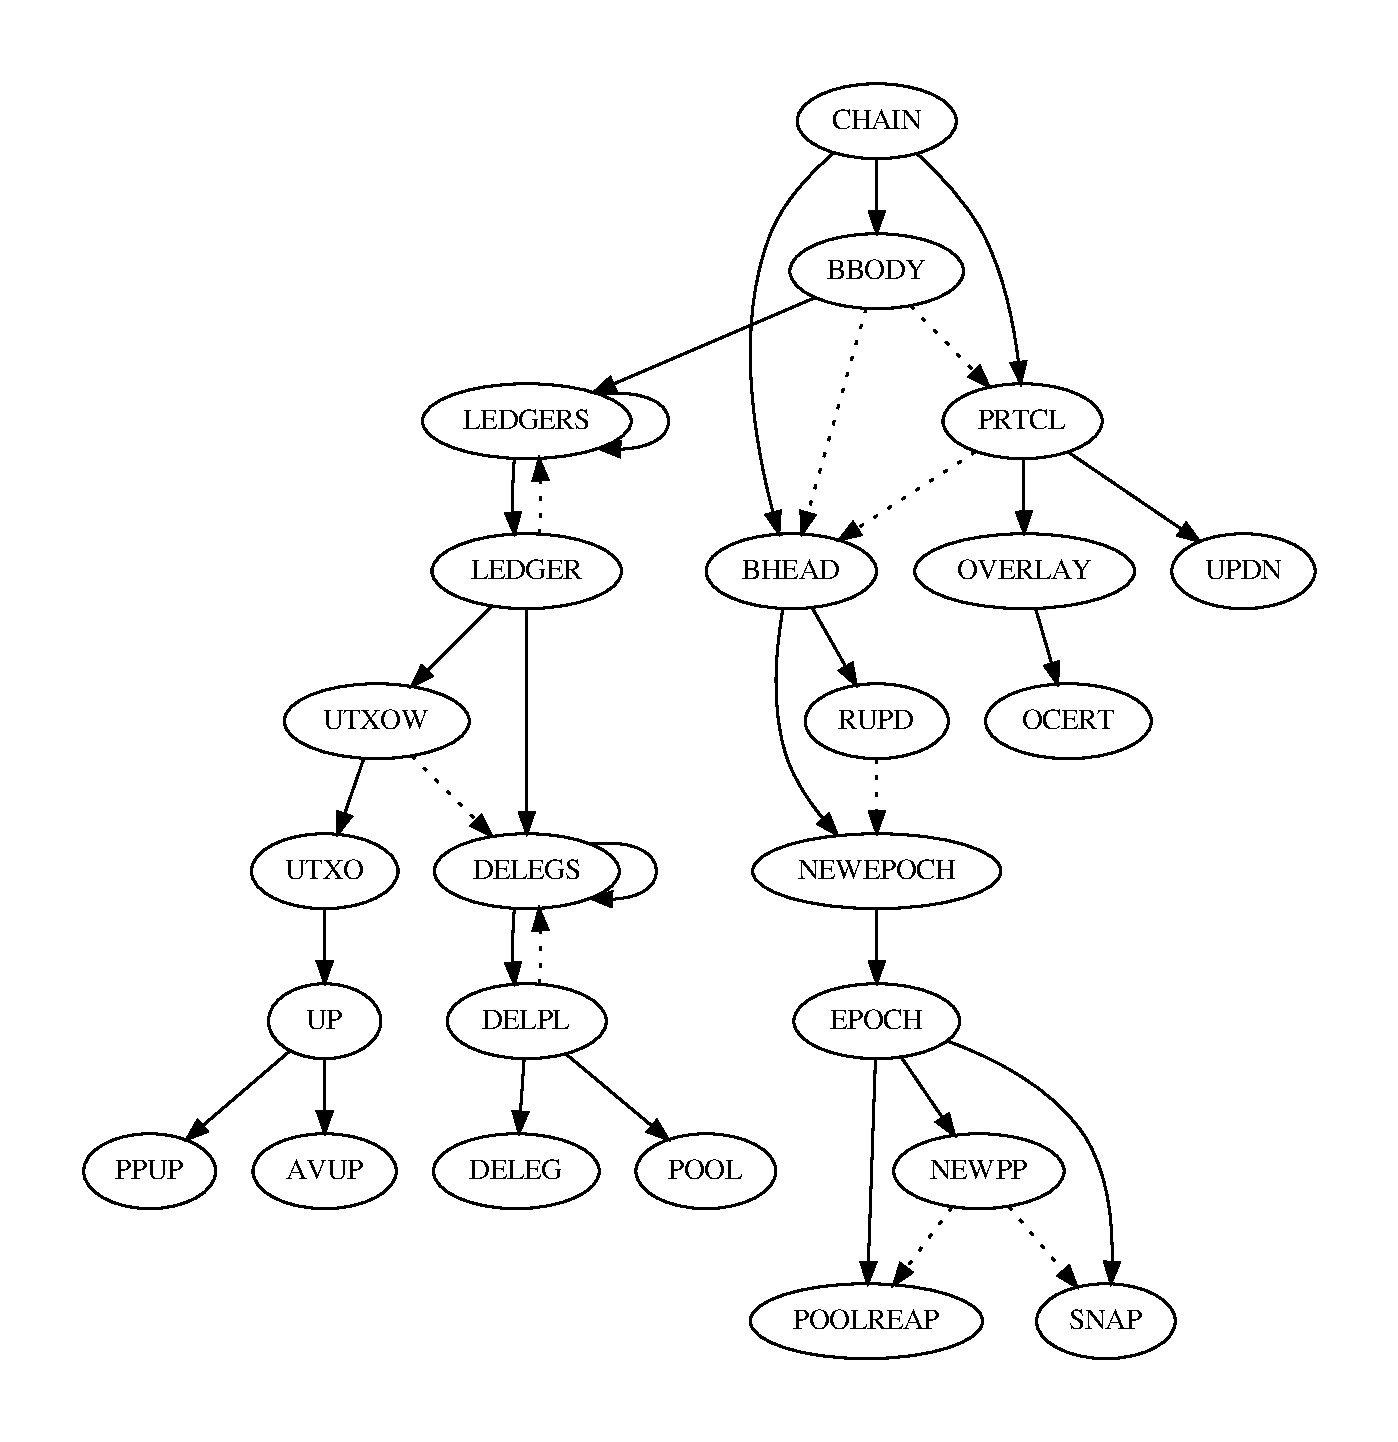
\includegraphics[width=\textwidth]{rules}
  \caption{STS Rules, Sub-Rules and Dependencies}
  \label{fig:sts-rules-dependencies}
\end{figure}

%%% Local Variables:
%%% mode: latex
%%% TeX-master: "ledger-spec"
%%% End:

In this section we discuss the properties which we want the ledger to have. One
goal is to include these properties in the executable specification for doing
property-based testing or formal verification.

\subsection{Validity of a Ledger State}
\label{sec:valid-ledg-state}

Many properties only make sense when applied to a valid ledger state. In
informal terms, a valid ledger state $l$ can only be reached when starting from
an initial state $l_{0}$ (genesis state) and only executing state transition
rules as specified in Section~\ref{sec:state-trans-utxo-1} for UTxO or
Section~\ref{sec:delegation} for delegation.

\begin{figure}[ht]
  \centering
  \begin{align*}
    \genesisId & \in & \TxId \\
    \genesisTxOut & \in & \TxOut \\
    \genesisUTxO & \coloneqq & \{\genesisId, \emptyset\} \mapsto \genesisTxOut
    \\
    \ledgerState & \in & \left(
                         \begin{array}{c}
                           \UTxO \\
                           \DState \\
                           \PState
                         \end{array}
    \right)\\
               && \\
    \fun{getUTxO} & \in & \ledgerState \to \UTxO \\
    \fun{getUTxO} & \coloneqq & (\var{utxo}, \wcard, \wcard) \to \var{utxo}
  \end{align*}
  \caption{Valid Ledger State}
  \label{fig:valid-ledger}
\end{figure}

In Figure~\ref{fig:valid-ledger} \genesisId{} marks the transaction identifier
of the initial coin distribution, where \genesisTxOut{} represents the initial
UTxO. It should be noted that no corresponding inputs exists, i.e., the
transaction inputs are the empty set for the initial transaction. An element of
\ledgerState{} is a triplet of UTxO, stake delegation state (\DState) and
delegation pool state (\PState).

\begin{definition}[\textbf{Valid Ledger State}]
  \begin{multline*}
    \label{eq:2}
    \forall l_{0},..,l_{n} \in \ledgerState, l_{0} =
    \left(
      \begin{array}{c}
        \left\{
        \genesisUTxO
        \right\} \\
        \emptyset\\
        \emptyset\\
      \end{array}
    \right)  \\
    \implies \forall 0 < i \leq n, ((\exists c \in \DCert, l_{i-1}
    \trans{delegw}{c} l_{i}) \vee (\exists tx \in \Tx: l_{i-1} \trans{utxow}{tx}
    l_{i}))\\ \implies \applyFun{validLedgerState}(l_{n})
  \end{multline*}
  \label{def:valid-ledger-state}
\end{definition}

Definition~\ref{def:valid-ledger-state} defines a valid ledger state reachable
from the genesis state via valid UTxO, stake delegation or stake pool
transactions. This gives a constructive rule how to reach a valid ledger state.

\subsection{Ledger Properties}
\label{sec:ledger-properties}

The following properties state the desired features of updating a valid ledger
state.

\begin{property}[\textbf{Preserve Balance Modulo Fee}]
  \begin{multline*}
    \forall \var{l}, \var{l'} \in \ledgerState: \applyFun{validLedgerstate}{l}\\
    \implies \forall \var{tx} \in \Tx, \var{l} \trans{utxo}{tx} \var{l'}
    \implies \fun{balance}(\applyFun{getUTxO}{l}) =
    \fun{balance}(\applyFun{getUTxO}{l'}) + \applyFun{txfee}{tx}
  \end{multline*}
  \label{prop:ledger-properties-1}
\end{property}

Property~\ref{prop:ledger-properties-1} states that for each valid ledger $l$,
if a transaction $tx$ is added to the ledger via the state transition rule
$utxow$ to the new ledger state $l'$, the balance of the UTxOs in $l$ equals the
balance of the UTxOs in $l'$ minus the transaction fees.

\begin{property}[\textbf{Preserve Balance Restricted to TxIns in Balance of
    TxOuts}]
  \begin{multline*}
    \forall \var{l}, \var{l'} \in \ledgerState: \applyFun{validLedgerstate}{l}\\
    \implies \forall \var{tx} \in \Tx, \var{l} \trans{utxo}{tx} \var{l'}
    \implies \fun{balance}(\applyFun{txins}{tx} \restrictdom
    \applyFun{getUTxO}{l}) = \fun{balance}(\applyFun{txouts}{tx}) +
    \applyFun{txfee}{tx}
  \end{multline*}
  \label{prop:ledger-properties-2}
\end{property}

Property~\ref{prop:ledger-properties-2} states the more detailed relation of the
balances change. For ledgers $l, l'$ and a transaction $tx$ as above, the
balance of the UTxOs of $l$ restricted to those whose domain is in the set of
transaction inputs of $tx$ equals the balance of the transaction outputs of $tx$
minus the transaction fees.

\begin{property}[\textbf{Preserve Outputs of Transaction}]
  \begin{multline*}
    \forall \var{l}, \var{l'} \in \ledgerState: \applyFun{validLedgerstate}{l}\\
    \implies \forall \var{tx} \in \Tx, \var{l} \trans{utxo}{tx} \var{l'}
    \implies \forall \var{out} \in \applyFun{txouts}{tx}, out \in
    \applyFun{getUTxO}{l'}
  \end{multline*}
  \label{prop:ledger-properties-3}
\end{property}

Property~\ref{prop:ledger-properties-3} states that for every ledger states
$l, l'$ and transaction $tx$ as above, all output UTxOs of $tx$ are in the UTxO
set of $l'$, i.e., they are now available as unspent transaction output.

\begin{property}[\textbf{Eliminate Inputs of Transaction}]
  \begin{multline*}
    \forall \var{l}, \var{l'} \in \ledgerState: \applyFun{validLedgerstate}{l}\\
    \implies \forall \var{tx} \in \Tx, \var{l} \trans{utxo}{tx} \var{l'}
    \implies \forall \var{in} \in \applyFun{txins}{tx}, in \not\in
    \fun{dom}(\applyFun{getUTxO}{l'})
  \end{multline*}
  \label{prop:ledger-properties-4}
\end{property}

Property~\ref{prop:ledger-properties-4} states that for every ledger states
$l, l'$ and transaction $tx$ as above, all transaction inputs $in$ of $tx$ are
not in the domain of the UTxO set of $l'$, i.e., these are no longer available
to spend.

\begin{property}[\textbf{Completeness and Collision-Freeness of new Transaction
    Ids}]
  \begin{multline*}
    \forall \var{l}, \var{l'} \in \ledgerState: \applyFun{validLedgerstate}{l}\\
    \implies \forall \var{tx} \in \Tx, \var{l} \trans{utxo}{tx} \var{l'}
    \implies \forall utxo' \in \applyFun{txouts}{tx}, \var{utxo'} \in
    \applyFun{getUTxO}{l'} \wedge \\(\var{utxo'} = ((\var{txId'}, \wcard) \mapsto
    \wcard) \implies \forall \var{utxo} \in \applyFun{getUTxO}{l}, \var{utxo} =
    ((\var{txId}, \wcard) \mapsto \wcard) \implies \var{txId'} \neq \var{txId}
  \end{multline*}
  \label{prop:ledger-properties-5}
\end{property}

Property~\ref{prop:ledger-properties-5} states that for ledger states $l, l'$
and a transaction $tx$ as above, the UTxOs of $l'$ contain all newly created
UTxOs and the referred transaction id of each new UTxO is not used in the UTxO
set of $l$.

%%% Local Variables:
%%% mode: latex
%%% TeX-master: "ledger-spec"
%%% End:

\section{Non-Integral Calculations}
\label{sec:non-integr-calc}

In the ledger there are several cases where non-integral calculations are
required, particularly calculations relating to delegation transitions.

\subsection{Types of Non-Integral Calculations}
\label{sec:types-non-integral}

The specification employs non-integral calculations for different mathematical
operations. Table~\ref{tab:func-non-integral} shows the function and transition
rules that use non-integral calculations and which type.

\begin{table}[ht]
  \centering
  \begin{tabular}{lccccc}
    \toprule
    name & page & multiplication & division & exponential function & exponentiation \\
    \midrule
    \fun{refund}
         & \pageref{fig:functions:deposits-refunds} & \checkmark & & \checkmark & \\
    \fun{maxPool}
         & \pageref{fig:functions:rewards} & \checkmark & \checkmark && \\
    \fun{poolReward}
         & \pageref{fig:functions:rewards} & \checkmark & & \checkmark &
                                                                         \checkmark \\
    \fun{r_{leader}}
         & \pageref{fig:functions:reward-splitting} & \checkmark & \checkmark &&\\
         \fun{r_{member}}
         & \pageref{fig:functions:reward-splitting} & \checkmark & \checkmark
                                            &&\\
    \fun{rewardOnePool}
         & \pageref{fig:functions:reward-calc} & \checkmark & \checkmark &&\\
    \fun{REWARD}
         &\pageref{fig:rules:reward-update} & \checkmark &&& \\
    \bottomrule
  \end{tabular}
  \caption{Functions with Non-Integral Calculation}
  \label{tab:func-non-integral}
\end{table}

The transcendental exponential function is used in reward and refund calculation
to model the decay of the deposit values. The pool reward uses exponentiation to
calculate a pool's ranking.

The domain for the exponential function are the non-negative reals, more
precisely the distribution parameter $\lambda \in (0, \infty)$ multiplied by a
discrete non-negative duration $\delta$.

The domain of the base of the exponentiation in $\fun{poolReward}$ are the
non-negative reals resulting from the calculation in $\fun{movingAvg}$, the
exponent $\gamma$ is a constant taken from the protocol parameters.

\subsection{Implementation of Non-Integer Calculations}
\label{sec:impl-non-integ}

The large part consists of multiplication and division which can easily be done
using fractional arithmetic to the desired precision. The precision necessary is
bounded by the ability to represent a single lovelace in all calculations.

\subsubsection{Function Simplification}
\label{sec:funct-simpl}

The transcendental function $e^{x}$ can be approximated using different
approaches, depending on the desired accuracy. In general, one uses the
exponential laws $e^{x} = 1/e^{-x}$ and
$e^{x} = \left(e^{\frac{x}{n}} \right)^{n}, n \in \mathbb{N}$ to reduce the
approximation to the unit interval and apply fast integral exponentiation
afterwards.

Exponentiation is implemented using the law
$a^{b} = e^{\ln(a^{b})}= e^{b\ln(a)}$. This therefore requires being able to
calculate $e^{x}$ and $\ln(x)$. The approximation of the natural logarithm can
be approximated using different approaches, again, depending on the desired
accuracy. Most approximations work for $\ln(x), x \in [1, c)$ with some $c >
0$. One then uses the law $\log_{b}(x) = \log_{b}(\frac{x}{b^{n}}b^{n})$ where
$n \in \mathbb{N}$ is chosen in such a way that $\frac{x}{b^{n}} \in [1,
c)$. Using this, one can separate the calculation of the integral and decimal
part as follows:

\begin{equation*}
  \log_{b}(\frac{x}{b^{n}}b^{n})=\log_{b}(b^{n}) + \log_{b}(\frac{x}{b^{n}})=
  n + \log(\frac{x}{b^{n}})
\end{equation*}

\subsubsection{Properties of Function Approximation}
\label{sec:prop-funct-appr-1}

There are several properties that approximations of the transcendental functions
are expected to have. In the following let $\ln'(x)$ be the approximation of
$\ln(x)$, $\exp'(x)$ be the approximation of $e^{x}$ and $x\star y$ the approximation
of $x^{y}$.

\begin{property}[\textbf{monotonicity}]
  \label{prop:monotone}
  Both $\exp'$ and $\ln'$ must be monotone on their respective domains.
\end{property}

In order to guarantee correctness of the approximations, we also require that
the mathematical laws are fulfilled. For some small $\epsilon > 0$, define
$x \approx y \Leftrightarrow \lvert x - y\rvert < \epsilon$.

\begin{property}[\textbf{Mathematical Laws}]
  \label{prop:ln-laws}
  The following mathematical laws state the requirements for the approximations
  of the $\ln'$ and $\exp'$ function:
  \begin{itemize}
  \item $\ln'(x\cdot y) \approx \ln'(x) + \ln'(y)$
  \item $\ln'(x^{y}) \approx y\cdot \ln'(x)$
  \item $\ln'(\exp'(x)) \approx \exp'(\ln'(x)) \approx x$
  \item $x, y \in [0,1] \implies x \star y \in [0, 1]$
  \item $x, y, z \in [0,1], x > 0 \implies
    (z\star\frac{1}{x})\star y \approx (z\star y)\star\frac{1}{x}$
  \item $\exp'(x + y) = \exp'(x) + \exp'(y)$
  \end{itemize}
\end{property}

%%% Local Variables:
%%% mode: latex
%%% TeX-master: "ledger-spec"
%%% End:


\newpage

\begin{appendix}
  \section{Proofs}
\label{sec:proofs}

\newif\ifproofs
% \proofstrue comment in to include generated proofs

For the proofs we use the automated theorem prover
MetiTarski~\cite{DBLP:journals/jar/AkbarpourP10} which is specialized for proofs
over real arithmetic, including elementary functions.

\begin{proof}
The property~(\ref{prop:minimal-refund}) (p.~\pageref{prop:minimal-refund}) for
the minimal refund can be proven automatically via

\begin{verbatim}
fof(minimal_refund, conjecture,
! [Dmin, Lambda, Delta, Dval] :
((Dmin : (=0,1=) & Lambda > 0 & Delta > 0 & Dval > 0
=>
Dval*Dmin >= 0 &
(Dval * (Dmin + (1 - Dmin) * exp(-Lambda * Delta))) : (=Dval * Dmin, Dval=)))).

fof(floor_lower_upper, conjecture,
! [X] :
(X >= 0 => X - 1 <= floor(X) & floor(X) <= X)).
\end{verbatim}
  \verb|minimal_refund| shows that the resulting value is within the interval
  $[d_{val}\cdot d_{min}, d_{val}]$ and that $d_{val}\cdot d_{min}$ is
  non-negative, while \verb|floor_lower_upper| shows that the floor of a value
  $x$ has an upper bound $x$ and lower bound $x - 1$.

\ifproofs
\begin{verbatim}
SZS output start CNFRefutation for minRefund.tptp
cnf(lgen_le_neg, axiom, (X <= Y | ~ lgen(0, X, Y))).

cnf(leq_left_divide_mul_pos, axiom, (Y * Z < X | X / Z <= Y | Z <= 0)).

cnf(interval_intro, axiom,
    (~ lgen(R, A, X) | ~ lgen(S, X, B) | interval(R, A, S, B, X))).

cnf(interval_elim1, axiom, (~ interval(R, A, S, B, X) | lgen(R, A, X))).

cnf(interval_elim2, axiom, (~ interval(R, A, S, B, X) | lgen(S, X, B))).

cnf(exp_upper_bound_cf2, axiom,
    (0 <= X | ~ lgen(R, (X ^ 2 + 6 * X + 12) / (X ^ 2 - 6 * X + 12), Y) |
     lgen(R, exp(X), Y))).

fof(minimal_refund, conjecture,
    (! [Dmin, Lambda, Delta, Dval] :
       ((interval(0, 0, 0, 1, Dmin) & 0 < Lambda & 0 < Delta & 0 < Dval) =>
        (0 <= Dval * Dmin &
         interval(0, Dval * Dmin, 0, Dval,
                  Dval * (Dmin + (1 - Dmin) * exp(-Lambda * Delta))))))).

fof(subgoal_0, plain,
    (! [Dmin, Lambda, Delta, Dval] :
       ((interval(0, 0, 0, 1, Dmin) & 0 < Lambda & 0 < Delta & 0 < Dval) =>
        0 <= Dval * Dmin)), inference(strip, [], [minimal_refund])).

fof(subgoal_1, plain,
    (! [Dmin, Lambda, Delta, Dval] :
       (((interval(0, 0, 0, 1, Dmin) & 0 < Lambda & 0 < Delta & 0 < Dval) &
         0 <= Dval * Dmin) =>
        interval(0, Dval * Dmin, 0, Dval,
                 Dval * (Dmin + (1 - Dmin) * exp(-Lambda * Delta))))),
    inference(strip, [], [minimal_refund])).

fof(negate_0_0, plain,
    (~ ! [Dmin, Lambda, Delta, Dval] :
         ((interval(0, 0, 0, 1, Dmin) & 0 < Lambda & 0 < Delta &
           0 < Dval) => 0 <= Dval * Dmin)),
    inference(negate, [], [subgoal_0])).

fof(normalize_0_0, plain,
    (? [Delta, Dmin, Dval, Lambda] :
       (0 < Delta & 0 < Dval & 0 < Lambda & Dval * Dmin < 0 &
        interval(0, 0, 0, 1, Dmin))),
    inference(canonicalize, [], [negate_0_0])).

fof(normalize_0_1, plain,
    (skoDvalC2 * skoDminC2 < 0 & 0 < skoDeltaC2 & 0 < skoDvalC2 &
     0 < skoLambdaC2 & interval(0, 0, 0, 1, skoDminC2)),
    inference(skolemize, [], [normalize_0_0])).

fof(normalize_0_2, plain, (interval(0, 0, 0, 1, skoDminC2)),
    inference(conjunct, [], [normalize_0_1])).

fof(normalize_0_3, plain, (skoDvalC2 * skoDminC2 < 0),
    inference(conjunct, [], [normalize_0_1])).

fof(normalize_0_4, plain, (0 < skoLambdaC2),
    inference(conjunct, [], [normalize_0_1])).

fof(normalize_0_5, plain, (0 < skoDvalC2),
    inference(conjunct, [], [normalize_0_1])).

fof(normalize_0_6, plain, (0 < skoDeltaC2),
    inference(conjunct, [], [normalize_0_1])).

cnf(refute_0_0, plain, (interval(0, 0, 0, 1, skoDminC2)),
    inference(canonicalize, [], [normalize_0_2])).

cnf(refute_0_1, plain,
    (~ interval(0, 0, 0, 1, skoDminC2) | lgen(0, 0, skoDminC2)),
    inference(subst, [], [interval_elim1])).

cnf(refute_0_2, plain, (lgen(0, 0, skoDminC2)),
    inference(resolve, [], [refute_0_0, refute_0_1])).

cnf(refute_0_3, plain, (0 <= skoDminC2),
    inference(arithmetic, [], [refute_0_2])).

cnf(refute_0_4, plain, (skoDvalC2 * skoDminC2 < 0),
    inference(canonicalize, [], [normalize_0_3])).

cnf(refute_0_5, plain, (0 < skoDvalC2 * (skoDminC2 * -1)),
    inference(arithmetic, [], [refute_0_4])).

cnf(refute_0_6, plain, (0 < skoLambdaC2),
    inference(canonicalize, [], [normalize_0_4])).

cnf(refute_0_7, plain, (0 < skoDvalC2),
    inference(canonicalize, [], [normalize_0_5])).

cnf(refute_0_8, plain, (0 < skoDeltaC2),
    inference(canonicalize, [], [normalize_0_6])).

cnf(refute_0_9, plain, (skoDminC2 < 0),
    inference(decision, [],
              [refute_0_5, refute_0_6, refute_0_7, refute_0_8])).

cnf(refute_0_10, plain, ($false),
    inference(resolve, [], [refute_0_3, refute_0_9])).

fof(negate_1_0, plain,
    (~ ! [Dmin, Lambda, Delta, Dval] :
         (((interval(0, 0, 0, 1, Dmin) & 0 < Lambda & 0 < Delta &
            0 < Dval) & 0 <= Dval * Dmin) =>
          interval(0, Dval * Dmin, 0, Dval,
                   Dval * (Dmin + (1 - Dmin) * exp(-Lambda * Delta))))),
    inference(negate, [], [subgoal_1])).

fof(normalize_1_0, plain,
    (? [Delta, Dmin, Dval, Lambda] :
       (0 < Delta & 0 < Dval & 0 < Lambda &
        ~ interval(0, Dval * Dmin, 0, Dval,
                   Dval * (Dmin + (1 - Dmin) * exp(-Lambda * Delta))) &
        0 <= Dval * Dmin & interval(0, 0, 0, 1, Dmin))),
    inference(canonicalize, [], [negate_1_0])).

fof(normalize_1_1, plain,
    (0 < skoDeltaC3 & 0 < skoDvalC3 & 0 < skoLambdaC3 &
     ~ interval(0, skoDvalC3 * skoDminC3, 0, skoDvalC3,
                skoDvalC3 *
                (skoDminC3 +
                 (1 - skoDminC3) * exp(-skoLambdaC3 * skoDeltaC3))) &
     0 <= skoDvalC3 * skoDminC3 & interval(0, 0, 0, 1, skoDminC3)),
    inference(skolemize, [], [normalize_1_0])).

fof(normalize_1_2, plain,
    (~ interval(0, skoDvalC3 * skoDminC3, 0, skoDvalC3,
                skoDvalC3 *
                (skoDminC3 +
                 (1 - skoDminC3) * exp(-skoLambdaC3 * skoDeltaC3)))),
    inference(conjunct, [], [normalize_1_1])).

fof(normalize_1_3, plain, (interval(0, 0, 0, 1, skoDminC3)),
    inference(conjunct, [], [normalize_1_1])).

fof(normalize_1_4, plain, (0 <= skoDvalC3 * skoDminC3),
    inference(conjunct, [], [normalize_1_1])).

fof(normalize_1_5, plain, (0 < skoLambdaC3),
    inference(conjunct, [], [normalize_1_1])).

fof(normalize_1_6, plain, (0 < skoDvalC3),
    inference(conjunct, [], [normalize_1_1])).

fof(normalize_1_7, plain, (0 < skoDeltaC3),
    inference(conjunct, [], [normalize_1_1])).

cnf(refute_1_0, plain,
    (1 *
     (12 +
      skoLambdaC3 *
      (skoDeltaC3 * 6 + skoLambdaC3 * (skoDeltaC3 * skoDeltaC3))) <
     12 +
     skoLambdaC3 *
     (skoDeltaC3 * -6 + skoLambdaC3 * (skoDeltaC3 * skoDeltaC3)) |
     12 +
     skoLambdaC3 *
     (skoDeltaC3 * 6 + skoLambdaC3 * (skoDeltaC3 * skoDeltaC3)) <= 0 |
     (12 +
      skoLambdaC3 *
      (skoDeltaC3 * -6 + skoLambdaC3 * (skoDeltaC3 * skoDeltaC3))) /
     (12 +
      skoLambdaC3 *
      (skoDeltaC3 * 6 + skoLambdaC3 * (skoDeltaC3 * skoDeltaC3))) <= 1),
    inference(subst, [], [leq_left_divide_mul_pos])).

cnf(refute_1_1, plain,
    (~ lgen(0, exp(X_000190), X_000191) | exp(X_000190) <= X_000191),
    inference(subst, [], [lgen_le_neg])).

cnf(refute_1_2, plain,
    (~ lgen(0,
            (X_000190 ^ 2 + 6 * X_000190 + 12) /
            (X_000190 ^ 2 - 6 * X_000190 + 12), X_000191) | 0 <= X_000190 |
     lgen(0, exp(X_000190), X_000191)),
    inference(subst, [], [exp_upper_bound_cf2])).

cnf(refute_1_3, plain,
    (~ lgen(0,
            (X_000190 ^ 2 + 6 * X_000190 + 12) /
            (X_000190 ^ 2 - 6 * X_000190 + 12), X_000191) | 0 <= X_000190 |
     exp(X_000190) <= X_000191),
    inference(resolve, [], [refute_1_2, refute_1_1])).

cnf(refute_1_4, plain,
    (X_000191 <
     (12 + X_000190 * (6 + X_000190)) / (12 + X_000190 * (-6 + X_000190)) |
     0 <= X_000190 | exp(X_000190) <= X_000191),
    inference(arithmetic, [], [refute_1_3])).

cnf(refute_1_5, plain,
    (1 <
     (12 +
      skoLambdaC3 * (skoDeltaC3 * -1) *
      (6 + skoLambdaC3 * (skoDeltaC3 * -1))) /
     (12 +
      skoLambdaC3 * (skoDeltaC3 * -1) *
      (-6 + skoLambdaC3 * (skoDeltaC3 * -1))) |
     0 <= skoLambdaC3 * (skoDeltaC3 * -1) |
     exp(skoLambdaC3 * (skoDeltaC3 * -1)) <= 1),
    inference(subst, [], [refute_1_4])).

cnf(refute_1_6, plain,
    (~ interval(0, skoDvalC3 * skoDminC3, 0, skoDvalC3,
                skoDvalC3 *
                (skoDminC3 +
                 (1 - skoDminC3) * exp(-skoLambdaC3 * skoDeltaC3)))),
    inference(canonicalize, [], [normalize_1_2])).

cnf(refute_1_7, plain,
    (~ interval(0, skoDvalC3 * skoDminC3, 0, skoDvalC3,
                skoDvalC3 * skoDminC3 +
                exp(skoLambdaC3 * (skoDeltaC3 * -1)) *
                (skoDvalC3 * (1 + skoDminC3 * -1)))),
    inference(arithmetic, [], [refute_1_6])).

cnf(refute_1_8, plain,
    (~ lgen(0, skoDvalC3 * skoDminC3,
            skoDvalC3 * skoDminC3 +
            exp(skoLambdaC3 * (skoDeltaC3 * -1)) *
            (skoDvalC3 * (1 + skoDminC3 * -1))) |
     ~ lgen(0,
            skoDvalC3 * skoDminC3 +
            exp(skoLambdaC3 * (skoDeltaC3 * -1)) *
            (skoDvalC3 * (1 + skoDminC3 * -1)), skoDvalC3) |
     interval(0, skoDvalC3 * skoDminC3, 0, skoDvalC3,
              skoDvalC3 * skoDminC3 +
              exp(skoLambdaC3 * (skoDeltaC3 * -1)) *
              (skoDvalC3 * (1 + skoDminC3 * -1)))),
    inference(subst, [], [interval_intro])).

cnf(refute_1_9, plain,
    (~ lgen(0, skoDvalC3 * skoDminC3,
            skoDvalC3 * skoDminC3 +
            exp(skoLambdaC3 * (skoDeltaC3 * -1)) *
            (skoDvalC3 * (1 + skoDminC3 * -1))) |
     ~ lgen(0,
            skoDvalC3 * skoDminC3 +
            exp(skoLambdaC3 * (skoDeltaC3 * -1)) *
            (skoDvalC3 * (1 + skoDminC3 * -1)), skoDvalC3)),
    inference(resolve, [], [refute_1_8, refute_1_7])).

cnf(refute_1_10, plain,
    (0 <
     exp(skoLambdaC3 * (skoDeltaC3 * -1)) *
     (skoDvalC3 * (-1 + skoDminC3)) |
     skoDvalC3 * (1 + skoDminC3 * -1) <
     exp(skoLambdaC3 * (skoDeltaC3 * -1)) *
     (skoDvalC3 * (1 + skoDminC3 * -1))),
    inference(arithmetic, [], [refute_1_9])).

cnf(refute_1_11, plain,
    (0 <
     exp(skoLambdaC3 * (skoDeltaC3 * -1)) *
     (skoDvalC3 * (-1 + skoDminC3)) |
     exp(skoLambdaC3 * (skoDeltaC3 * -1)) *
     (skoDvalC3 * (-1 + skoDminC3)) <= 0),
    introduced(tautology, [assume])).

cnf(refute_1_12, plain,
    (0 < 0 | skoDvalC3 * (-1 + skoDminC3) < 0 |
     0 < skoDvalC3 * (-1 + skoDminC3) |
     exp(skoLambdaC3 * (skoDeltaC3 * -1)) *
     (skoDvalC3 * (-1 + skoDminC3)) <= 0),
    inference(split, [], [refute_1_11])).

cnf(refute_1_13, plain,
    (0 < skoDvalC3 * (-1 + skoDminC3) |
     0 < skoDvalC3 * (1 + skoDminC3 * -1) |
     exp(skoLambdaC3 * (skoDeltaC3 * -1)) *
     (skoDvalC3 * (-1 + skoDminC3)) <= 0),
    inference(arithmetic, [], [refute_1_12])).

cnf(refute_1_14, plain,
    (exp(skoLambdaC3 * (skoDeltaC3 * -1)) <
     0 / (skoDvalC3 * (-1 + skoDminC3)) |
     0 <= skoDvalC3 * (-1 + skoDminC3) |
     exp(skoLambdaC3 * (skoDeltaC3 * -1)) *
     (skoDvalC3 * (-1 + skoDminC3)) <= 0),
    inference(split, [], [refute_1_11])).

cnf(refute_1_15, plain,
    (exp(skoLambdaC3 * (skoDeltaC3 * -1)) *
     (skoDvalC3 * (-1 + skoDminC3)) <= 0 |
     skoDvalC3 * (1 + skoDminC3 * -1) <= 0),
    inference(arithmetic, [], [refute_1_14])).

cnf(refute_1_16, plain,
    (0 < skoDvalC3 * (-1 + skoDminC3) |
     exp(skoLambdaC3 * (skoDeltaC3 * -1)) *
     (skoDvalC3 * (-1 + skoDminC3)) <= 0),
    inference(resolve, [], [refute_1_15, refute_1_13])).

cnf(refute_1_17, plain, (interval(0, 0, 0, 1, skoDminC3)),
    inference(canonicalize, [], [normalize_1_3])).

cnf(refute_1_18, plain,
    (~ interval(0, 0, 0, 1, skoDminC3) | lgen(0, skoDminC3, 1)),
    inference(subst, [], [interval_elim2])).

cnf(refute_1_19, plain, (lgen(0, skoDminC3, 1)),
    inference(resolve, [], [refute_1_17, refute_1_18])).

cnf(refute_1_20, plain, (skoDminC3 <= 1),
    inference(arithmetic, [], [refute_1_19])).

cnf(refute_1_21, plain, (0 <= skoDvalC3 * skoDminC3),
    inference(canonicalize, [], [normalize_1_4])).

cnf(refute_1_22, plain, (skoDvalC3 * (skoDminC3 * -1) <= 0),
    inference(arithmetic, [], [refute_1_21])).

cnf(refute_1_23, plain, (0 < skoLambdaC3),
    inference(canonicalize, [], [normalize_1_5])).

cnf(refute_1_24, plain, (0 < skoDvalC3),
    inference(canonicalize, [], [normalize_1_6])).

cnf(refute_1_25, plain, (0 < skoDeltaC3),
    inference(canonicalize, [], [normalize_1_7])).

cnf(refute_1_26, plain, (skoDvalC3 * (-1 + skoDminC3) <= 0),
    inference(decision, [],
              [refute_1_20, refute_1_22, refute_1_23, refute_1_24,
               refute_1_25])).

cnf(refute_1_27, plain,
    (exp(skoLambdaC3 * (skoDeltaC3 * -1)) *
     (skoDvalC3 * (-1 + skoDminC3)) <= 0),
    inference(resolve, [], [refute_1_26, refute_1_16])).

cnf(refute_1_28, plain,
    (skoDvalC3 * (1 + skoDminC3 * -1) <
     exp(skoLambdaC3 * (skoDeltaC3 * -1)) *
     (skoDvalC3 * (1 + skoDminC3 * -1))),
    inference(resolve, [], [refute_1_27, refute_1_10])).

cnf(refute_1_29, plain,
    (skoDvalC3 * (1 + skoDminC3 * -1) /
     (skoDvalC3 * (1 + skoDminC3 * -1)) <
     exp(skoLambdaC3 * (skoDeltaC3 * -1)) |
     skoDvalC3 * (1 + skoDminC3 * -1) <= 0),
    inference(split, [], [refute_1_28])).

cnf(refute_1_30, plain,
    (1 < exp(skoLambdaC3 * (skoDeltaC3 * -1)) |
     skoDvalC3 * (1 + skoDminC3 * -1) <= 0 | 1 = skoDminC3 |
     skoDvalC3 = 0), inference(arithmetic, [], [refute_1_29])).

cnf(refute_1_31, plain,
    (0 < skoDvalC3 * (1 + skoDminC3 * -1) | 1 = skoDminC3 | skoDvalC3 = 0),
    inference(decision, [],
              [refute_1_25, refute_1_24, refute_1_23, refute_1_22,
               refute_1_20])).

cnf(refute_1_32, plain,
    (1 < exp(skoLambdaC3 * (skoDeltaC3 * -1)) | 1 = skoDminC3 |
     skoDvalC3 = 0), inference(resolve, [], [refute_1_30, refute_1_31])).

cnf(refute_1_33, plain, (skoDvalC3 != 0 | 1 = skoDminC3),
    inference(decision, [],
              [refute_1_25, refute_1_24, refute_1_23, refute_1_22,
               refute_1_20])).

cnf(refute_1_34, plain,
    (1 < exp(skoLambdaC3 * (skoDeltaC3 * -1)) | 1 = skoDminC3),
    inference(resolve, [], [refute_1_32, refute_1_33])).

cnf(refute_1_35, plain,
    (1 <
     (12 +
      skoLambdaC3 * (skoDeltaC3 * -1) *
      (6 + skoLambdaC3 * (skoDeltaC3 * -1))) /
     (12 +
      skoLambdaC3 * (skoDeltaC3 * -1) *
      (-6 + skoLambdaC3 * (skoDeltaC3 * -1))) |
     0 <= skoLambdaC3 * (skoDeltaC3 * -1) | 1 = skoDminC3),
    inference(resolve, [], [refute_1_5, refute_1_34])).

cnf(refute_1_36, plain,
    (1 <
     (12 +
      skoLambdaC3 *
      (skoDeltaC3 * -6 + skoLambdaC3 * (skoDeltaC3 * skoDeltaC3))) /
     (12 +
      skoLambdaC3 *
      (skoDeltaC3 * 6 + skoLambdaC3 * (skoDeltaC3 * skoDeltaC3))) |
     skoLambdaC3 * skoDeltaC3 <= 0 | 1 = skoDminC3),
    inference(arithmetic, [], [refute_1_35])).

cnf(refute_1_37, plain,
    (skoDvalC3 * (1 + skoDminC3 * -1) < 0 |
     0 < skoDvalC3 * (1 + skoDminC3 * -1)),
    inference(split, [], [refute_1_28])).

cnf(refute_1_38, plain,
    (0 < skoDvalC3 * (-1 + skoDminC3) |
     0 < skoDvalC3 * (1 + skoDminC3 * -1)),
    inference(arithmetic, [], [refute_1_37])).

cnf(refute_1_39, plain,
    (0 < skoDvalC3 * (1 + skoDminC3 * -1) |
     skoDvalC3 * (-1 + skoDminC3) <= 0),
    inference(decision, [],
              [refute_1_25, refute_1_24, refute_1_23, refute_1_22,
               refute_1_20])).

cnf(refute_1_40, plain, (0 < skoDvalC3 * (1 + skoDminC3 * -1)),
    inference(resolve, [], [refute_1_39, refute_1_38])).

cnf(refute_1_41, plain, (0 < skoLambdaC3 * skoDeltaC3 | 1 = skoDminC3),
    inference(decision, [],
              [refute_1_40, refute_1_25, refute_1_24, refute_1_23,
               refute_1_22, refute_1_20])).

cnf(refute_1_42, plain,
    (1 <
     (12 +
      skoLambdaC3 *
      (skoDeltaC3 * -6 + skoLambdaC3 * (skoDeltaC3 * skoDeltaC3))) /
     (12 +
      skoLambdaC3 *
      (skoDeltaC3 * 6 + skoLambdaC3 * (skoDeltaC3 * skoDeltaC3))) |
     1 = skoDminC3), inference(resolve, [], [refute_1_36, refute_1_41])).

cnf(refute_1_43, plain, (1 != skoDminC3),
    inference(decision, [],
              [refute_1_40, refute_1_25, refute_1_24, refute_1_23,
               refute_1_22, refute_1_20])).

cnf(refute_1_44, plain,
    (1 <
     (12 +
      skoLambdaC3 *
      (skoDeltaC3 * -6 + skoLambdaC3 * (skoDeltaC3 * skoDeltaC3))) /
     (12 +
      skoLambdaC3 *
      (skoDeltaC3 * 6 + skoLambdaC3 * (skoDeltaC3 * skoDeltaC3)))),
    inference(resolve, [], [refute_1_42, refute_1_43])).

cnf(refute_1_45, plain,
    (1 *
     (12 +
      skoLambdaC3 *
      (skoDeltaC3 * 6 + skoLambdaC3 * (skoDeltaC3 * skoDeltaC3))) <
     12 +
     skoLambdaC3 *
     (skoDeltaC3 * -6 + skoLambdaC3 * (skoDeltaC3 * skoDeltaC3)) |
     12 +
     skoLambdaC3 *
     (skoDeltaC3 * 6 + skoLambdaC3 * (skoDeltaC3 * skoDeltaC3)) <= 0),
    inference(resolve, [], [refute_1_0, refute_1_44])).

cnf(refute_1_46, plain,
    (0 < skoLambdaC3 * (skoDeltaC3 * -12) |
     skoLambdaC3 *
     (skoDeltaC3 * 6 + skoLambdaC3 * (skoDeltaC3 * skoDeltaC3)) <= -12),
    inference(arithmetic, [], [refute_1_45])).

cnf(refute_1_47, plain,
    (0 < skoLambdaC3 * (skoDeltaC3 * -12) |
     -12 <
     skoLambdaC3 *
     (skoDeltaC3 * 6 + skoLambdaC3 * (skoDeltaC3 * skoDeltaC3))),
    inference(decision, [],
              [refute_1_40, refute_1_25, refute_1_24, refute_1_23,
               refute_1_22, refute_1_20])).

cnf(refute_1_48, plain, (0 < skoLambdaC3 * (skoDeltaC3 * -12)),
    inference(resolve, [], [refute_1_46, refute_1_47])).

cnf(refute_1_49, plain, (skoLambdaC3 * (skoDeltaC3 * -12) <= 0),
    inference(decision, [],
              [refute_1_40, refute_1_25, refute_1_24, refute_1_23,
               refute_1_22, refute_1_20])).

cnf(refute_1_50, plain, ($false),
    inference(resolve, [], [refute_1_49, refute_1_48])).
SZS output end CNFRefutation for minRefund.tptp
\end{verbatim}

\begin{verbatim}
SZS output start CNFRefutation for floor.tptp
cnf(lgen_le_neg, axiom, (X <= Y | ~ lgen(0, X, Y))).

cnf(floor_upper_bound, axiom, (~ lgen(R, X, Y) | lgen(R, floor(X), Y))).

cnf(floor_lower_bound, axiom, (X - 1 < Y | lgen(R, Y, floor(X)))).

fof(floor_lower_upper, conjecture,
    (! [X] : (0 <= X => (X - 1 <= floor(X) & floor(X) <= X)))).

fof(subgoal_0, plain, (! [X] : (0 <= X => X - 1 <= floor(X))),
    inference(strip, [], [floor_lower_upper])).

fof(subgoal_1, plain,
    (! [X] : ((0 <= X & X - 1 <= floor(X)) => floor(X) <= X)),
    inference(strip, [], [floor_lower_upper])).

fof(negate_0_0, plain, (~ ! [X] : (0 <= X => X - 1 <= floor(X))),
    inference(negate, [], [subgoal_0])).

fof(normalize_0_0, plain, (? [X] : (floor(X) < X - 1 & 0 <= X)),
    inference(canonicalize, [], [negate_0_0])).

fof(normalize_0_1, plain, (floor(skoXC2) < skoXC2 - 1 & 0 <= skoXC2),
    inference(skolemize, [], [normalize_0_0])).

fof(normalize_0_2, plain, (floor(skoXC2) < skoXC2 - 1),
    inference(conjunct, [], [normalize_0_1])).

cnf(refute_0_0, plain, (floor(skoXC2) < skoXC2 - 1),
    inference(canonicalize, [], [normalize_0_2])).

cnf(refute_0_1, plain, (floor(skoXC2) < -1 + skoXC2),
    inference(arithmetic, [], [refute_0_0])).

cnf(refute_0_2, plain,
    (~ lgen(0, X_000012, floor(X_000011)) | X_000012 <= floor(X_000011)),
    inference(subst, [], [lgen_le_neg])).

cnf(refute_0_3, plain,
    (X_000011 - 1 < X_000012 | lgen(0, X_000012, floor(X_000011))),
    inference(subst, [], [floor_lower_bound])).

cnf(refute_0_4, plain,
    (X_000011 - 1 < X_000012 | X_000012 <= floor(X_000011)),
    inference(resolve, [], [refute_0_3, refute_0_2])).

cnf(refute_0_5, plain,
    (-1 + X_000011 < X_000012 | X_000012 <= floor(X_000011)),
    inference(arithmetic, [], [refute_0_4])).

cnf(refute_0_6, plain,
    (-1 + skoXC2 < -1 + skoXC2 | -1 + skoXC2 <= floor(skoXC2)),
    inference(subst, [], [refute_0_5])).

cnf(refute_0_7, plain, (-1 + skoXC2 < -1 + skoXC2),
    inference(resolve, [], [refute_0_6, refute_0_1])).

cnf(refute_0_8, plain, ($false), inference(arithmetic, [], [refute_0_7])).

fof(negate_1_0, plain,
    (~ ! [X] : ((0 <= X & X - 1 <= floor(X)) => floor(X) <= X)),
    inference(negate, [], [subgoal_1])).

fof(normalize_1_0, plain,
    (? [X] : (X < floor(X) & 0 <= X & X - 1 <= floor(X))),
    inference(canonicalize, [], [negate_1_0])).

fof(normalize_1_1, plain,
    (skoXC3 < floor(skoXC3) & 0 <= skoXC3 & skoXC3 - 1 <= floor(skoXC3)),
    inference(skolemize, [], [normalize_1_0])).

fof(normalize_1_2, plain, (skoXC3 < floor(skoXC3)),
    inference(conjunct, [], [normalize_1_1])).

cnf(refute_1_0, plain, (skoXC3 < floor(skoXC3)),
    inference(canonicalize, [], [normalize_1_2])).

cnf(refute_1_1, plain,
    (~ lgen(0, floor(X_000034), X_000035) | floor(X_000034) <= X_000035),
    inference(subst, [], [lgen_le_neg])).

cnf(refute_1_2, plain,
    (~ lgen(0, X_000034, X_000035) | lgen(0, floor(X_000034), X_000035)),
    inference(subst, [], [floor_upper_bound])).

cnf(refute_1_3, plain,
    (~ lgen(0, X_000034, X_000035) | floor(X_000034) <= X_000035),
    inference(resolve, [], [refute_1_2, refute_1_1])).

cnf(refute_1_4, plain, (X_000035 < X_000034 | floor(X_000034) <= X_000035),
    inference(arithmetic, [], [refute_1_3])).

cnf(refute_1_5, plain, (skoXC3 < skoXC3 | floor(skoXC3) <= skoXC3),
    inference(subst, [], [refute_1_4])).

cnf(refute_1_6, plain, (skoXC3 < skoXC3),
    inference(resolve, [], [refute_1_5, refute_1_0])).

cnf(refute_1_7, plain, ($false), inference(arithmetic, [], [refute_1_6])).
SZS output end CNFRefutation for floor.tptp
\end{verbatim}
\fi
\end{proof}


\begin{proof}
  For the property~(\ref{prop:reward-splitting})
  (p.~\pageref{prop:reward-splitting}) for reward splitting between we actually
  show a stronger one, by removing the floor function. Using the fractional
  values we get an upper bound for the real value and showing that this upper
  bound is bounded by $\hat{f}$ we show that the real value is also bounded by
  $\hat{f}$. To eliminate the sum, we use the identity
  $\frac{s + \sum_{j}t_{j}}{\sigma} = 1$, see the definition of $\sigma$
  in~\cite{delegation_design}. Using this, we show for $\hat{f} > c$

  \begin{multline*}
    0 \leq c + (\hat{f} - c)\cdot (m + (1 - m))\cdot \frac{s}{\sigma} +
    \sum_{j}(\hat{f}-c)\cdot(1-m)\cdot\frac{t_{j}}{\sigma} \leq \hat{f} \\
    \Leftrightarrow
    0\leq c + (\hat{f}-c)\cdot m \cdot \frac{s}{\sigma} + (\hat{f}
    -c)\cdot(1-m)\cdot\frac{s + \sum_{j}t_{j}}{\sigma} \leq \hat{f} \\
    \Leftrightarrow
    0\leq c + (\hat{f}-c)\cdot m \cdot \frac{s}{\sigma} + (\hat{f}
    -c)\cdot(1-m) \leq \hat{f} \\
  \end{multline*}

  This can be proven automatically using

\begin{verbatim}
fof(reward_splitting, conjecture,
! [C, F, M, S, Sigma] :
(
M : (=0, 1=) & C >= 0 & F > C & Sigma : (0, 1=) & S : (=0, Sigma=)
=>
C + (F - C) * M * S / Sigma + (F - C) * (1 - M) <= F &
0 <= C + (F - C) * M * S / Sigma + (F - C) * (1 - M))).
\end{verbatim}

  \ifproofs
\begin{verbatim}
SZS output start CNFRefutation for rewardsplit.tptp
cnf(leq_left_divide_mul_pos, axiom, (Y * Z < X | X / Z <= Y | Z <= 0)).

cnf(leq_right_divide_mul_pos, axiom, (Y < X * Z | X <= Y / Z | Z <= 0)).

cnf(leq_left_divide_mul_neg, axiom, (Y * Z < X | Y <= X / Z | 0 <= Z)).

cnf(leq_right_divide_mul_neg, axiom, (Y < X * Z | Y / Z <= X | 0 <= Z)).

cnf(interval_elim1, axiom, (~ interval(R, A, S, B, X) | lgen(R, A, X))).

cnf(interval_elim2, axiom, (~ interval(R, A, S, B, X) | lgen(S, X, B))).

fof(reward_splitting, conjecture,
    (! [C, F, M, S, Sigma] :
       ((interval(0, 0, 0, 1, M) & 0 <= C & C < F &
         interval(1, 0, 0, 1, Sigma) & interval(0, 0, 0, Sigma, S)) =>
        (C + (F - C) * M * S / Sigma + (F - C) * (1 - M) <= F &
         0 <= C + (F - C) * M * S / Sigma + (F - C) * (1 - M))))).

fof(subgoal_0, plain,
    (! [C, F, M, S, Sigma] :
       ((interval(0, 0, 0, 1, M) & 0 <= C & C < F &
         interval(1, 0, 0, 1, Sigma) & interval(0, 0, 0, Sigma, S)) =>
        C + (F - C) * M * S / Sigma + (F - C) * (1 - M) <= F)),
    inference(strip, [], [reward_splitting])).

fof(subgoal_1, plain,
    (! [C, F, M, S, Sigma] :
       (((interval(0, 0, 0, 1, M) & 0 <= C & C < F &
          interval(1, 0, 0, 1, Sigma) & interval(0, 0, 0, Sigma, S)) &
         C + (F - C) * M * S / Sigma + (F - C) * (1 - M) <= F) =>
        0 <= C + (F - C) * M * S / Sigma + (F - C) * (1 - M))),
    inference(strip, [], [reward_splitting])).

fof(negate_0_0, plain,
    (~ ! [C, F, M, S, Sigma] :
         ((interval(0, 0, 0, 1, M) & 0 <= C & C < F &
           interval(1, 0, 0, 1, Sigma) & interval(0, 0, 0, Sigma, S)) =>
          C + (F - C) * M * S / Sigma + (F - C) * (1 - M) <= F)),
    inference(negate, [], [subgoal_0])).

fof(normalize_0_0, plain,
    (? [C, F, M, S, Sigma] :
       (C < F & F < C + (F - C) * M * S / Sigma + (F - C) * (1 - M) &
        0 <= C & interval(0, 0, 0, Sigma, S) & interval(0, 0, 0, 1, M) &
        interval(1, 0, 0, 1, Sigma))),
    inference(canonicalize, [], [negate_0_0])).

fof(normalize_0_1, plain,
    (skoFC2 <
     skoCC2 + (skoFC2 - skoCC2) * skoMC2 * skoSC2 / skoSigmaC2 +
     (skoFC2 - skoCC2) * (1 - skoMC2) & skoCC2 < skoFC2 & 0 <= skoCC2 &
     interval(0, 0, 0, 1, skoMC2) & interval(0, 0, 0, skoSigmaC2, skoSC2) &
     interval(1, 0, 0, 1, skoSigmaC2)),
    inference(skolemize, [], [normalize_0_0])).

fof(normalize_0_2, plain, (interval(0, 0, 0, skoSigmaC2, skoSC2)),
    inference(conjunct, [], [normalize_0_1])).

fof(normalize_0_3, plain, (interval(1, 0, 0, 1, skoSigmaC2)),
    inference(conjunct, [], [normalize_0_1])).

fof(normalize_0_4, plain, (interval(0, 0, 0, 1, skoMC2)),
    inference(conjunct, [], [normalize_0_1])).

fof(normalize_0_5, plain,
    (skoFC2 <
     skoCC2 + (skoFC2 - skoCC2) * skoMC2 * skoSC2 / skoSigmaC2 +
     (skoFC2 - skoCC2) * (1 - skoMC2)),
    inference(conjunct, [], [normalize_0_1])).

fof(normalize_0_6, plain, (0 <= skoCC2),
    inference(conjunct, [], [normalize_0_1])).

fof(normalize_0_7, plain, (skoCC2 < skoFC2),
    inference(conjunct, [], [normalize_0_1])).

cnf(refute_0_0, plain, (interval(0, 0, 0, skoSigmaC2, skoSC2)),
    inference(canonicalize, [], [normalize_0_2])).

cnf(refute_0_1, plain,
    (~ interval(0, 0, 0, skoSigmaC2, skoSC2) |
     lgen(0, skoSC2, skoSigmaC2)), inference(subst, [], [interval_elim2])).

cnf(refute_0_2, plain, (lgen(0, skoSC2, skoSigmaC2)),
    inference(resolve, [], [refute_0_0, refute_0_1])).

cnf(refute_0_3, plain, (skoSC2 <= skoSigmaC2),
    inference(arithmetic, [], [refute_0_2])).

cnf(refute_0_4, plain, (interval(1, 0, 0, 1, skoSigmaC2)),
    inference(canonicalize, [], [normalize_0_3])).

cnf(refute_0_5, plain,
    (~ interval(1, 0, 0, 1, skoSigmaC2) | lgen(1, 0, skoSigmaC2)),
    inference(subst, [], [interval_elim1])).

cnf(refute_0_6, plain, (lgen(1, 0, skoSigmaC2)),
    inference(resolve, [], [refute_0_4, refute_0_5])).

cnf(refute_0_7, plain, (0 < skoSigmaC2),
    inference(arithmetic, [], [refute_0_6])).

cnf(refute_0_8, plain,
    (~ interval(0, 0, 0, skoSigmaC2, skoSC2) | lgen(0, 0, skoSC2)),
    inference(subst, [], [interval_elim1])).

cnf(refute_0_9, plain, (lgen(0, 0, skoSC2)),
    inference(resolve, [], [refute_0_0, refute_0_8])).

cnf(refute_0_10, plain, (0 <= skoSC2),
    inference(arithmetic, [], [refute_0_9])).

cnf(refute_0_11, plain, (interval(0, 0, 0, 1, skoMC2)),
    inference(canonicalize, [], [normalize_0_4])).

cnf(refute_0_12, plain,
    (~ interval(0, 0, 0, 1, skoMC2) | lgen(0, 0, skoMC2)),
    inference(subst, [], [interval_elim1])).

cnf(refute_0_13, plain, (lgen(0, 0, skoMC2)),
    inference(resolve, [], [refute_0_11, refute_0_12])).

cnf(refute_0_14, plain, (0 <= skoMC2),
    inference(arithmetic, [], [refute_0_13])).

cnf(refute_0_15, plain,
    (skoFC2 <
     skoCC2 + (skoFC2 - skoCC2) * skoMC2 * skoSC2 / skoSigmaC2 +
     (skoFC2 - skoCC2) * (1 - skoMC2)),
    inference(canonicalize, [], [normalize_0_5])).

cnf(refute_0_16, plain,
    (skoMC2 * (skoCC2 * -1 + skoFC2) <
     skoSC2 * (skoMC2 * (skoCC2 * -1 + skoFC2)) / skoSigmaC2),
    inference(arithmetic, [], [refute_0_15])).

cnf(refute_0_17, plain,
    (skoSC2 * (skoMC2 * (skoCC2 * -1 + skoFC2)) <
     skoMC2 * (skoCC2 * -1 + skoFC2) * skoSigmaC2 | 0 <= skoSigmaC2 |
     skoSC2 * (skoMC2 * (skoCC2 * -1 + skoFC2)) / skoSigmaC2 <=
     skoMC2 * (skoCC2 * -1 + skoFC2)),
    inference(subst, [], [leq_right_divide_mul_neg])).

cnf(refute_0_18, plain,
    (skoSC2 * (skoMC2 * (skoCC2 * -1 + skoFC2)) <
     skoMC2 * (skoCC2 * -1 + skoFC2) * skoSigmaC2 | 0 <= skoSigmaC2),
    inference(resolve, [], [refute_0_17, refute_0_16])).

cnf(refute_0_19, plain,
    (skoSC2 * (skoMC2 * (skoCC2 * -1 + skoFC2)) <
     skoSigmaC2 * (skoMC2 * (skoCC2 * -1 + skoFC2)) | 0 <= skoSigmaC2),
    inference(arithmetic, [], [refute_0_18])).

cnf(refute_0_20, plain,
    (skoMC2 * (skoCC2 * -1 + skoFC2) * skoSigmaC2 <
     skoSC2 * (skoMC2 * (skoCC2 * -1 + skoFC2)) |
     skoSC2 * (skoMC2 * (skoCC2 * -1 + skoFC2)) / skoSigmaC2 <=
     skoMC2 * (skoCC2 * -1 + skoFC2) | skoSigmaC2 <= 0),
    inference(subst, [], [leq_left_divide_mul_pos])).

cnf(refute_0_21, plain,
    (skoMC2 * (skoCC2 * -1 + skoFC2) * skoSigmaC2 <
     skoSC2 * (skoMC2 * (skoCC2 * -1 + skoFC2)) | skoSigmaC2 <= 0),
    inference(resolve, [], [refute_0_20, refute_0_16])).

cnf(refute_0_22, plain,
    (skoSC2 * (skoMC2 * (skoCC2 + skoFC2 * -1)) <
     skoSigmaC2 * (skoMC2 * (skoCC2 + skoFC2 * -1)) | skoSigmaC2 <= 0),
    inference(arithmetic, [], [refute_0_21])).

cnf(refute_0_23, plain, (0 <= skoCC2),
    inference(canonicalize, [], [normalize_0_6])).

cnf(refute_0_24, plain, (skoCC2 < skoFC2),
    inference(canonicalize, [], [normalize_0_7])).

cnf(refute_0_25, plain, (skoSigmaC2 < skoSC2),
    inference(decision, [],
              [refute_0_7, refute_0_10, refute_0_14, refute_0_19,
               refute_0_22, refute_0_23, refute_0_24])).

cnf(refute_0_26, plain, ($false),
    inference(resolve, [], [refute_0_3, refute_0_25])).

fof(negate_1_0, plain,
    (~ ! [C, F, M, S, Sigma] :
         (((interval(0, 0, 0, 1, M) & 0 <= C & C < F &
            interval(1, 0, 0, 1, Sigma) & interval(0, 0, 0, Sigma, S)) &
           C + (F - C) * M * S / Sigma + (F - C) * (1 - M) <= F) =>
          0 <= C + (F - C) * M * S / Sigma + (F - C) * (1 - M))),
    inference(negate, [], [subgoal_1])).

fof(normalize_1_0, plain,
    (? [C, F, M, S, Sigma] :
       (C < F & C + (F - C) * M * S / Sigma + (F - C) * (1 - M) < 0 &
        0 <= C & C + (F - C) * M * S / Sigma + (F - C) * (1 - M) <= F &
        interval(0, 0, 0, Sigma, S) & interval(0, 0, 0, 1, M) &
        interval(1, 0, 0, 1, Sigma))),
    inference(canonicalize, [], [negate_1_0])).

fof(normalize_1_1, plain,
    (skoCC3 + (skoFC3 - skoCC3) * skoMC3 * skoSC3 / skoSigmaC3 +
     (skoFC3 - skoCC3) * (1 - skoMC3) < 0 & skoCC3 < skoFC3 & 0 <= skoCC3 &
     skoCC3 + (skoFC3 - skoCC3) * skoMC3 * skoSC3 / skoSigmaC3 +
     (skoFC3 - skoCC3) * (1 - skoMC3) <= skoFC3 &
     interval(0, 0, 0, 1, skoMC3) & interval(0, 0, 0, skoSigmaC3, skoSC3) &
     interval(1, 0, 0, 1, skoSigmaC3)),
    inference(skolemize, [], [normalize_1_0])).

fof(normalize_1_2, plain, (interval(0, 0, 0, 1, skoMC3)),
    inference(conjunct, [], [normalize_1_1])).

fof(normalize_1_3, plain, (interval(1, 0, 0, 1, skoSigmaC3)),
    inference(conjunct, [], [normalize_1_1])).

fof(normalize_1_4, plain, (interval(0, 0, 0, skoSigmaC3, skoSC3)),
    inference(conjunct, [], [normalize_1_1])).

fof(normalize_1_5, plain,
    (skoCC3 + (skoFC3 - skoCC3) * skoMC3 * skoSC3 / skoSigmaC3 +
     (skoFC3 - skoCC3) * (1 - skoMC3) < 0),
    inference(conjunct, [], [normalize_1_1])).

fof(normalize_1_6, plain, (0 <= skoCC3),
    inference(conjunct, [], [normalize_1_1])).

fof(normalize_1_7, plain, (skoCC3 < skoFC3),
    inference(conjunct, [], [normalize_1_1])).

cnf(refute_1_0, plain, (interval(0, 0, 0, 1, skoMC3)),
    inference(canonicalize, [], [normalize_1_2])).

cnf(refute_1_1, plain,
    (~ interval(0, 0, 0, 1, skoMC3) | lgen(0, skoMC3, 1)),
    inference(subst, [], [interval_elim2])).

cnf(refute_1_2, plain, (lgen(0, skoMC3, 1)),
    inference(resolve, [], [refute_1_0, refute_1_1])).

cnf(refute_1_3, plain, (skoMC3 <= 1),
    inference(arithmetic, [], [refute_1_2])).

cnf(refute_1_4, plain, (interval(1, 0, 0, 1, skoSigmaC3)),
    inference(canonicalize, [], [normalize_1_3])).

cnf(refute_1_5, plain,
    (~ interval(1, 0, 0, 1, skoSigmaC3) | lgen(1, 0, skoSigmaC3)),
    inference(subst, [], [interval_elim1])).

cnf(refute_1_6, plain, (lgen(1, 0, skoSigmaC3)),
    inference(resolve, [], [refute_1_4, refute_1_5])).

cnf(refute_1_7, plain, (0 < skoSigmaC3),
    inference(arithmetic, [], [refute_1_6])).

cnf(refute_1_8, plain, (interval(0, 0, 0, skoSigmaC3, skoSC3)),
    inference(canonicalize, [], [normalize_1_4])).

cnf(refute_1_9, plain,
    (~ interval(0, 0, 0, skoSigmaC3, skoSC3) | lgen(0, 0, skoSC3)),
    inference(subst, [], [interval_elim1])).

cnf(refute_1_10, plain, (lgen(0, 0, skoSC3)),
    inference(resolve, [], [refute_1_8, refute_1_9])).

cnf(refute_1_11, plain, (0 <= skoSC3),
    inference(arithmetic, [], [refute_1_10])).

cnf(refute_1_12, plain,
    (~ interval(0, 0, 0, 1, skoMC3) | lgen(0, 0, skoMC3)),
    inference(subst, [], [interval_elim1])).

cnf(refute_1_13, plain, (lgen(0, 0, skoMC3)),
    inference(resolve, [], [refute_1_0, refute_1_12])).

cnf(refute_1_14, plain, (0 <= skoMC3),
    inference(arithmetic, [], [refute_1_13])).

cnf(refute_1_15, plain,
    (skoCC3 + (skoFC3 - skoCC3) * skoMC3 * skoSC3 / skoSigmaC3 +
     (skoFC3 - skoCC3) * (1 - skoMC3) < 0),
    inference(canonicalize, [], [normalize_1_5])).

cnf(refute_1_16, plain,
    (skoSC3 * (skoMC3 * (skoCC3 * -1 + skoFC3)) / skoSigmaC3 <
     skoFC3 * -1 + skoMC3 * (skoCC3 * -1 + skoFC3)),
    inference(arithmetic, [], [refute_1_15])).

cnf(refute_1_17, plain,
    ((skoFC3 * -1 + skoMC3 * (skoCC3 * -1 + skoFC3)) * skoSigmaC3 <
     skoSC3 * (skoMC3 * (skoCC3 * -1 + skoFC3)) | 0 <= skoSigmaC3 |
     skoFC3 * -1 + skoMC3 * (skoCC3 * -1 + skoFC3) <=
     skoSC3 * (skoMC3 * (skoCC3 * -1 + skoFC3)) / skoSigmaC3),
    inference(subst, [], [leq_left_divide_mul_neg])).

cnf(refute_1_18, plain,
    ((skoFC3 * -1 + skoMC3 * (skoCC3 * -1 + skoFC3)) * skoSigmaC3 <
     skoSC3 * (skoMC3 * (skoCC3 * -1 + skoFC3)) | 0 <= skoSigmaC3),
    inference(resolve, [], [refute_1_17, refute_1_16])).

cnf(refute_1_19, plain,
    (skoSC3 * (skoMC3 * (skoCC3 + skoFC3 * -1)) <
     skoSigmaC3 * (skoFC3 + skoMC3 * (skoCC3 + skoFC3 * -1)) |
     0 <= skoSigmaC3), inference(arithmetic, [], [refute_1_18])).

cnf(refute_1_20, plain,
    (skoSC3 * (skoMC3 * (skoCC3 * -1 + skoFC3)) <
     (skoFC3 * -1 + skoMC3 * (skoCC3 * -1 + skoFC3)) * skoSigmaC3 |
     skoFC3 * -1 + skoMC3 * (skoCC3 * -1 + skoFC3) <=
     skoSC3 * (skoMC3 * (skoCC3 * -1 + skoFC3)) / skoSigmaC3 |
     skoSigmaC3 <= 0), inference(subst, [], [leq_right_divide_mul_pos])).

cnf(refute_1_21, plain,
    (skoSC3 * (skoMC3 * (skoCC3 * -1 + skoFC3)) <
     (skoFC3 * -1 + skoMC3 * (skoCC3 * -1 + skoFC3)) * skoSigmaC3 |
     skoSigmaC3 <= 0), inference(resolve, [], [refute_1_20, refute_1_16])).

cnf(refute_1_22, plain,
    (skoSC3 * (skoMC3 * (skoCC3 * -1 + skoFC3)) <
     skoSigmaC3 * (skoFC3 * -1 + skoMC3 * (skoCC3 * -1 + skoFC3)) |
     skoSigmaC3 <= 0), inference(arithmetic, [], [refute_1_21])).

cnf(refute_1_23, plain, (0 <= skoCC3),
    inference(canonicalize, [], [normalize_1_6])).

cnf(refute_1_24, plain, (skoCC3 < skoFC3),
    inference(canonicalize, [], [normalize_1_7])).

cnf(refute_1_25, plain, (1 < skoMC3),
    inference(decision, [],
              [refute_1_7, refute_1_11, refute_1_14, refute_1_19,
               refute_1_22, refute_1_23, refute_1_24])).

cnf(refute_1_26, plain, ($false),
    inference(resolve, [], [refute_1_3, refute_1_25])).
SZS output end CNFRefutation for rewardsplit.tptp
\end{verbatim}
  \fi
\end{proof}

%%% Local Variables:
%%% mode: latex
%%% TeX-master: "ledger-spec"
%%% End:

\end{appendix}


\addcontentsline{toc}{section}{References}
\bibliographystyle{plainnat}
\bibliography{references}

\end{document}
